\documentclass[12pt, a4paper]{report} %report
\usepackage{amsfonts, amsmath, amsthm}
\usepackage{indentfirst}
\usepackage[utf8x]{inputenc}
\usepackage{multirow}
\usepackage[romanian]{babel}
\usepackage{combelow}
\usepackage[table]{xcolor}
\usepackage{graphicx}
\usepackage{tocloft}
\usepackage{algorithm, algorithmicx, algpseudocode}
\usepackage{tocloft}
\usepackage{caption}
\usepackage[top=2.5cm, bottom=2.5cm, left=2.5cm, right=2.5cm]{geometry}
\usepackage{hyperref}
\usepackage{subcaption}

\newcommand*{\utb}{\item[{
\includegraphics[width=0.15cm]{imagini/patrat.png}}]}
\renewcommand{\cftchapleader}{\cftdotfill{\cftdotsep}}
\captionsetup[table]{name=Tabelul}

\makeatletter
\renewcommand{\ALG@name}{Algoritm}
\makeatother

\makeatletter
\renewcommand{\maketitle}{\bgroup\setlength{\parindent}{0pt}
	\begin{flushleft}
		\textbf{\@title}
		
		\@author
		
		\vspace{10mm}
		\@date
	\end{flushleft}\egroup
}
\makeatother

\title{\begin{minipage} {0.3\textwidth}
		{{
\includegraphics[width=6cm]{imagini/sigla.png} }}%
	\end{minipage}
	\hfill
	\begin{minipage}{0.3\textwidth}
		\fontsize{10pt}{6pt}\selectfont
			Programul de studii:\\
			Informatica aplicata\\
	\end{minipage}
	\vspace*{7\baselineskip}\\
	\begin{center}
			\fontsize{22pt}{6pt}\selectfont
		\bf Lucrare de licen\c{t}\u{a}\\
		\vspace{5mm}
		Acustica spa\c{t}iilor interioare folosind metoda Ray-Tracing
		\vspace*{30\baselineskip}
	\end{center}
	}

\author{\fontsize{15pt}{6pt}\selectfont
	{\bf Autor:} \hspace{5.1cm}Lixandru Andreea-Bianca\\
	\vspace{3mm}
	{\bf Mentori:} \hspace{4.6cm}Nil\u{a} Costin\\
	\vspace{3mm}
	\hspace{7cm}Gorobievschi Sebastian\\
	\vspace{3mm}
	\hspace{7cm}(Siemens Industry Software)\\
	\vspace{3mm}
	{\bf Coordonator \c{S}tiin\c{t}ific:} \hspace{1cm}Lect. Dr. B\u{a}icoianu Alexandra}

\date{\begin{center} Bra\c{s}ov, 2021 \end{center}}

\begin{document}
	
	\maketitle	
	\thispagestyle{empty} %single page disable page number
	
	\newpage
	\tableofcontents
	\thispagestyle{empty}

		\thispagestyle{empty}
	\begin{center}
		\bf{ABSTRACT}
	\end{center}
	
	
	urmeaza sa ma ocup de partea asta 
	
	
	\addcontentsline{toc}{chapter}{Scopul lucr\u arii}
	\chapter*{Scopul lucr\u arii}
			\^{I}n ultimele decenii, au fost dezvoltate multiple modele ce calculeaz\u{a} modul de propagare al undelor acustice \^{i}n spa\c{t}iul virtual. Din acest motiv am ales s\u{a} dezvolt o aplica\c{t}ie software care modeleaz\u{a} propagarea sunetului în încăperi folosind metoda Ray-Tracing. Exist\u{a} multiple motive pentru dezvoltarea și îmbunătățirea model\u{a}rii acustice \^{i}n \^{i}nc\u{a}peri. Aceast\u{a} lucrare va prezenta ce presupune implementarea unui model acustic, at\^{a}t din punct de vedere fizic, c\^{a}t \c{s}i din punct de vedere geometric \c{s}i vizual. Mai mult de at\^{a}t, va fi prezentat\u{a} \c{s}i implementarea unui model de acest tip, dar \c{s}i rezultatele ob\c{t}inute, însoțite de o serie de experimente și o validare a modelului acustic. Evident, nici un model care promovează propagarea sunetului \^{i}ntr-un mediu virtual nu va imita 1 la 1 realitatea. Totu\c{s}i, se \^{i}ncearc\u{a} g\u{a}sirea unui algoritm c\^{a}t mai fezabil.

	Atunci când vorbim despre sunetul din cadrul unei încăperi poate una dintre cele mai importante probleme este să ne dăm seama unde ar trebui să poziționăm sursa audio pentru ca sunetul să fie auzit peste tot și la o calitate cât mai bună. Pentru inginerii acustici propagarea sunetului într-o încăpere este un subiect foarte important, întrucât aceștia au nevoie să știe cum trebuie să realizeze încăperi precum hale, mall-uri, aeroporturi astfel încât acestea să se afle în parametrii acustici pentru a nu deteriora sănătatea urechii omului ce lucrează în medii expuse. De asemenea, atunci când inginerul acustic realizează o biserică sau o catedrală, acesta este nevoit să țină cont de problema propagării sunetul astfel încât acesta să fie auzit peste tot și clar, chiar dacă formele din interiorul acestora variază foarte mult.
	
	În ziua de azi industria jocurilor a început să se dezvolte foarte mult datorită rolului esențial pe care aceasta îl ocupă în societate. Din acest motiv, au fost realizate o serie de proiecte inovative menite să dezvolte și să promoveze importanța propagării sunetului în jocuri și realitate mixtă, problemă care ar putea fi rezolvată folosind o soluție precum cea promovată de această lucrare.
	
	Pe tema propagării sunetului în încăperi au fost realizate o mulțime de studii pentru a putea găsi un mod cât mai eficient și relevant de a rezolva această problemă. Fiind un subiect de mare interes în timpurile noastre am ales să dezvolt un model acustic menit să simuleze propagarea sunetului în spații interioare folosind metoda Ray-tracing. Lucrarea urmărește să prezinte modul în care a fost realizat modelul acustic, o serie de rezultate a unor experimente și validarea modelului folosind software-ul Simcenter 3D.
	
	Considerând aceste arii de interes, industria ingineriei acustice și industria jocurilor, am dorit să creez prin această lucrare un model acustic care să simuleze propagarea sunetului în încăperi pentru a veni în ajutorul celor care activează în cele două industrii.
		
	\addcontentsline{toc}{chapter}{Introducere}
	\chapter*{Introducere}
		Acustica este știința preocupată de producția, controlul, transmisia, recepția și efectele sunetului. Acest termen provine din limba greacă, de la cuvântul \textit{,,akoustos''}. Începând cu originile sale în studiul vibrațiilor mecanice și al radiației acestor vibrații prin unde mecanice, acustica este implicată în aproape toate domeniile vieții. A fost esențială în dezvoltarea culturii popoarele prin crearea instrumentelor muzicale.

Originea științei acusticii este atribuită, în general, filosofului grec Pitagora, ale cărui experimente asupra proprietăților corzilor vibrante care produc intervale muzicale plăcute au avut un merit atât de mare încât au condus la un sistem de acordare care îi poartă numele. Aristotel a sugerat corect că o undă sonoră se propagă în aer prin mișcarea aerului - o ipoteză bazată mai mult pe filosofie decât pe fizica experimentală; totuși, el a sugerat în mod incorect că frecvențele înalte se propagă mai repede decât frecvențele joase - o eroare care a persistat timp de multe secole \cite{istorie}.

Considerând toate acestea, ne putem da seama că omul a acordat permanent o importa\-nță deosebită domeniului acusticii. Întorși în zilele noastre, ne dăm seama că elaborarea unui model acustic este și astăzi un subiect de mare interes.

Urechea umană este sensibilă la vibrațiile aerului cu frecvențe între 20 Hz și 20 kHz și, odată cu vârsta, acest interval se restrânge. Modul în care percepem sunetul diferă de la o încăpere la alta și acest lucru se întâmplă datorită camerelor care au o anumită dimensiune și formă, sunt construite din diverse materiale și conțin suprafețe diferite.

Când discutăm despre o cameră, un aspect foarte important de reținut este unde ar trebui să poziționăm sursele audio și microfoanele pentru a obține cea mai bună calitate a sunetului și pentru a reduce cât mai mult posibil efectul de ecou și de reverberație. În interiorul unei camere, undele sonore lovesc diferite suprafețe care pot absorbi sau reflecta sunetul. Este foarte important pentru inginerii care proiectează modele acustice să aleagă materialele potrivite pentru a obține rezultate optime. De exemplu, fabricile și halele au multe suprafețe metalice care favorizează efectul de ecou. Acest fenomen poate fi verificat de inginerii care proiectează spațiile pentru a se asigura că încăperea respectă toate standardele, iar sănătatea persoanelor care lucrează în acele spații nu este compromisă.

Un model acustic va implica, în cel mai generic mod, simularea căilor pe care sunetul le parcurge de la sursă la destinație. Cel mai adesea, aceste modele propun rezolvarea integralei Helmoltz-Kirchoff \cite{kirchoff} utilizând diverse abordări de calcul, cum ar fi: soluții numerice la ecuațiile de undă, aproximări de frecvență înaltă la ecuația de undă și modele statistice bazate perceptiv. Modelul pe care l-am creat face parte din a doua categorie.

De obicei, termenul de Ray-Tracing este folosit pentru lumină, dar poate fi folosit și pentru sunet, întrucât atunci când avem frecvențe mari, undele sonore au o amplitudine foarte mică și deci le putem aproxima folosind raze. Din acest motiv, am folosit metoda Ray-Tracing pentru a crea un model acustic.

Această lucrare va presupune elaborarea unui model acustic pentru spațiile interioare folosind metoda Ray-Tracing, model care va conține patru etape principale: calcularea geometriei încăperii, realizarea calculelor fizice, post-procesarea datelor obținute și realizarea unei interfețe care să se ocupe de vizualizarea simulării acustice și a rezultatelor obținute de către model.

Pentru a putea evalua corectitudinea modelului au fost realizate două încăperi rectangulare și una sferică folosind platforma Unity. În interiorul acestora au fost plasate o serie de microfoane și o sursă audio. De asemenea, studiul propune un GUI (Graphical User Interface) ușor de folosit pentru a seta configurația dorită pentru fiecare încăpere și pentru a putea vizualiza rezultatele obținute de către modelul acustic. Mai mult de atât, ca să putem valida corectitudinea soluției am folosit software-ul Simcenter3D, o platformă de simulare complet integrată pentru modelarea, simularea și analizarea produselor și sistemelor complexe de inginerie.

Modelul acustic propus de această lucrare va presupune parcurgerea unor etape secven\-țiale, unde output-ul unei etape va reprezenta input-ul următoarei etape. Acesta va conține etapa de calcul geometric ce se va ocupa de simularea razelor și de modul în care acestea vor fi distribuite în încăpere, al doilea pas se va referi la calculele fizice, iar mai apoi va avea loc o etapă de post-procesare a datelor pentru a putea analiza rezultatele fizice obținute pentru fiecare microfon din încăpere.

Ideea acestei lucrări a pornit de la proiectul Triton oferit de Microsoft ce propune rezolvarea problemei propagării sunetului în jocuri și realitate mixtă. Acesta modelează fizic modul în care sunetul se propagă într-o scenă, având în vedere forma și materialele sale. Procedând astfel, modelează automat efecte imersive de propagare a sunetului precum ocluzia și reverberația sunetului. Proiectul Triton este unic în modelarea cu acuratețe a adevăratei fizice a undelor de sunet, inclusiv a difracției. Incubat de peste un deceniu de cercetări concentrate, este o tehnologie testată în luptă, livrată în titluri majore de jocuri precum Gears of War, Sea of Thieves și Borderlands 3. Proiectul Triton modelează fizica reală a undelor de propagare a sunetului prin spații 3D complexe. Sunetele sonore au lungimi de undă de la centimetri la metri, astfel încât efectele de undă trebuie modelate pentru a evita rezultate nenaturale \cite{triton}.

O altă sursă de inspirație a fost lucrarea lui David Oliva Elorza care vorbește despre modelarea acustică în încăperi folosind metoda Ray-Tracing. Autorul prezintă în studiul său noțiunile teoretice de care are nevoie un cititor specializat atunci când dorește să realizeze un model acustic, propune implementarea acestuia și o serie de evaluări ale modelului. Acesta discută o introducere generală a principiilor de propagare a sunetului și o discuție despre stadiul tehnicii în modelarea acustică a încăperilor \cite{elorza}. Față de ce propune Elorza în studiul său, această lucrare propune un mod diferit de distribuire, selecție și reducere al razelor.

În lucrarea \textit{Simulare computerizată a acusticii moscheilor și bisericilor bizantine} a lui Christoffer A. Weitze \cite{chris} este propus un model destinat simulărilor acustice în moscheele și bisericile bizantine, pe când în cadrul acestei lucrări este propus un model acustic mult mai generic.

Astfel, în capitolul ce urmează vor fi prezentate noțiunile teoretice necesare pentru a realiza un model acustic, după care va fi un capitol ce prezintă tehnologiile folosite, urmat de prezentarea modelului acustic implementat și o serie de experimente realizate folosind acest model. Penultimul capitol va conține validarea acestuia folosind software-ul Simcenter 3D, urmat de capitolul final unde se vor prezenta concluziile.

	\chapter{No\c{t}iuni teoretice necesare}
			\section{Sunetul}
	Sunetul reprezint\u{a} vibra\c{t}ia particulelor ce se propagă prin unde, \^{i}ntr-un mediu, fie el gazos, lichid sau solid \c{s}i prezint\u{a}, \^{i}n multe aspecte, dar nu \^{i}n toate, comportament similar cu alte mi\c{s}c\u{a}ri de und\u{a} pe care le \^{i}nt\^{a}lnim \^{i}n natur\u{a}, adic\u{a} undele ce se formează la suprafața apei \c{s}i undele de lumin\u{a}, ale c\u{a}ror fenomene de propagare sunt u\c{s}or de
	observat.
	 
	
	\^{I}n contextul propag\u{a}rii sunetului, aerul este mediul de interes despre care vom discuta atunci c\^{a}nd vorbim despre acustica \^{i}nc\u{a}perilor, iar perturbarea reprezint\u{a} o alterare a presiunii atmosferice peste \c{s}i sub valoarea sa medie, care produce o mi\c{s}care periodic\u{a} a moleculelor de aer \^{i}napoi \c{s}i \^{i}nainte de-a lungul aceleia\c{s}i direc\c{t}ii \^{i}n care se propag\u{a} unda (unde longitudinale).
	 
	
	Propagarea sunetului prin aer este ilustrat\u{a} în Figura \ref{Fig1}. \^{I}n partea superioar\u{a}
	este ilustrat\u{a} alterarea presiunii atmosferice, \^{i}n timp ce \^{i}n partea inferioar\u{a} este ilustrat\u{a} mi\c{s}carea moleculelor de aer asociate cu propagarea sunetului. Dac\u{a} intensitatea
	sunetului cre\c{s}te, gradientul presiunii cre\c{s}te \c{s}i, ca urmare, mai multe
	molecule de aer se afl\u{a} \^{i}n mi\c{s}care.
	
	\begin{figure}[!htb]
		\centering
		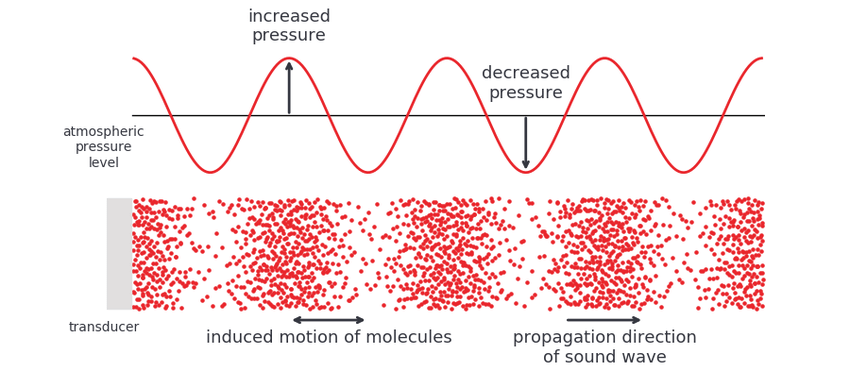
\includegraphics[width=1\linewidth]{imagini/propagareaSunetuluiInAer.png}
		\caption{Propagarea sunetului prin aer\cite{elorza}}
		\label{Fig1}
	\end{figure}

	Un principiu general, stabilit pentru prima dat\u{a} de Fermat, afirm\u{a} c\u{a} fiecare und\u{a} se propag\u{a} de la surs\u{a} c\u{a}tre receptor prin calea cea mai rapid\u{a}. Dac\u{a} mediul este omogen, precum consider\u{a}m c\u{a} este aerul, atunci viteza sunetului este uniform\u{a} prin acest mediu \c{s}i astfel calea cea mai rapid\u{a} devine totodat\u{a} \c{s}i cea mai scurt\u{a}.
	Viteza sunetului depinde doar de temperatur\u{a}, nu \c{s}i de alte propriet\u{a}\c{t}i precum presiunea \c{s}i densitatea. Astfel, putem observa \^{i}n Tabelul \ref{Tabel1} cum variaz\u{a} viteza \c{s}i densitatea sunetului \^{i}n func\c{t}ie de temperatur\u{a}.
	
	 
	\begin{table}[!htb]
		\centering		
	\begin{tabular}{|c|c|c|}
		\hline
		\bf{Temperatur\u{a} ($^{\circ}$C)} & \bf{Viteza sunetului $\left(\dfrac{m}{s} \right)$} & \bf{Densitatea aerului $\left(\dfrac{kg}{m^3}\right)$}\\
		\hline \hline
		
		30 & 349.02 & 1.1644\\
		\hline
		25 & 346.13 & 1.1839\\
		\hline
		20 & 343.21 & 1.2041\\
		\hline
		15 & 340.27 & 1.2250\\
		\hline
		10 & 337.31 & 1.2466\\
		\hline
		5 & 334.32 & 1.2690\\
		\hline
		0 & 331.30 & 1.2922\\
		\hline			
	\end{tabular}
	\caption{Efectul temperaturii asupra propriet\u{a}\c{t}ilor aerului\cite{temperaturaTabel}}
	\label{Tabel1}
	\end{table}

	{\it{Amplitudinea}} este valoarea absolut\u{a}, maxim\u{a}, a unei cantit\u{a}\c{t}i care variaz\u{a} periodic. Amplitudinile sunt exprimate fie ca valori instantanee, fie mai ales ca valori de v\^{a}rf. Aceasta reprezint\u{a} fluctua\c{t}ia sau deplasarea unei unde de la valoarea sa medie. \^{I}n cazul undelor sonore, particulele de aer sunt deplasate, iar aceast\u{a} amplitudine a sunetului este exprimat\u{a} ca intensitatea sunetului. Amplitudinea nu este influen\c{t}at\u{a} de frecven\c{t}\u{a}, de lungimea de und\u{a}, de perioada de timp sau de viteza sunetului \c{s}i nici invers.
	 
	{\it{Lungimea de und\u{a}}} este reprezentat\u{a} de distan\c{t}a dintre punctele consecutive corespunz\u{a}toare ale aceleia\c{s}i faze de und\u{a}, precum dou\u{a} creste adiacente. {\it{Viteza de propagare ($c$)}} a undei este dat\u{a} de lungimea de und\u{a}, pe care o vom nota cu $\lambda$, fiind distan\c{t}a parcurs\u{a} de val \^{i}ntre dou\u{a} instan\c{t}e de faz\u{a} egal\u{a} \c{s}i de timp, $T$, timpul necesar acestei distan\c{t}e.
	
	\begin{equation}
	c=\lambda/T
	\end{equation}
	 	
	Inversa perioadei este numit\u{a} {\it{frecven\c{t}\u{a} ($f$)}} \c{s}i indic\u{a} de c\^{a}te ori particulele de aer s-au mi\c{s}cat \^{i}napoi \c{s}i \^{i}nainte \^{i}ntr-o secund\u{a}. Frecven\c{t}a este m\u{a}surat\u{a} \^{i}n Hertz[Hz].
	
	\begin{equation}
	c=\lambda f
	\end{equation}	 
	
	O caracteristic\u{a} important\u{a} a unei unde sonore este {\it{faza}}, care specific\u{a} loca\c{t}ia unui punct \^{i}n cadrul unui ciclu de und\u{a} al unei forme de und\u{a} repetitive. \^{I}n majoritatea cazurilor, diferen\c{t}ele de faz\u{a} dintre undele sonore sunt mai importante dec\^{a} fazele \^{i}n sine. Diferen\c{t}a de faz\u{a} dintre dou\u{a} unde sonore cu aceea\c{s}i frecven\c{t}\u{a} care se deplaseaz\u{a} dincolo de o loca\c{t}ie fix\u{a} este dat\u{a} de diferen\c{t}a de timp dintre acelea\c{s}i pozi\c{t}ii \^{i}n cadrul ciclurilor de und\u{a} ale celor dou\u{a} sunete, exprimate ca o frac\c{t}iune dintr-un ciclu de und\u{a}. 	  
	
	Dou\u{a} unde sonore de aceea\c{s}i frecven\c{t}\u{a} care sunt perfect aliniate au o diferen\c{t}\u{a} de faz\u{a} de 0 \c{s}i se spune c\u{a} sunt ,,\^{i}n faz\u{a}". Dou\u{a} unde care sunt ,,\^{i}n faz\u{a}" se adaug\u{a} pentru a produce o und\u{a} sonor\u{a} cu o amplitudine egal\u{a} cu suma amplitudinilor celor dou\u{a} unde, precum în Figura \ref{Fig7}.

	\begin{figure}[!htb]
		\centering
		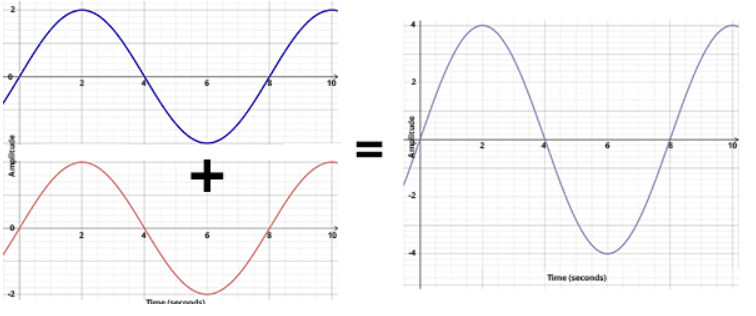
\includegraphics[width=10cm]{imagini/soundWaveGreaterAmplitude.png}
		\caption{Dou\u{a} unde sonore ,,\^{i}n faz\u{a}"}
		\label{Fig7}
	\end{figure}

	Dac\u{a} una dintre cele dou\u{a} unde sonore cu aceea\c{s}i frecven\c{t}\u{a} este deplasat\u{a} cu o jum\u{a}tate de ciclu fa\c{t}\u{a} de cealalt\u{a}, se spune c\u{a} undele sonore sunt ,,defazate". Dou\u{a} unde sunt ,,defazate" dac\u{a} se anuleaz\u{a} reciproc exact c\^{a}nd sunt adunate \^{i}mpreun\u{a}, precum în Figura \ref{Fig8}.

	\begin{figure}[!htb]
		\centering
		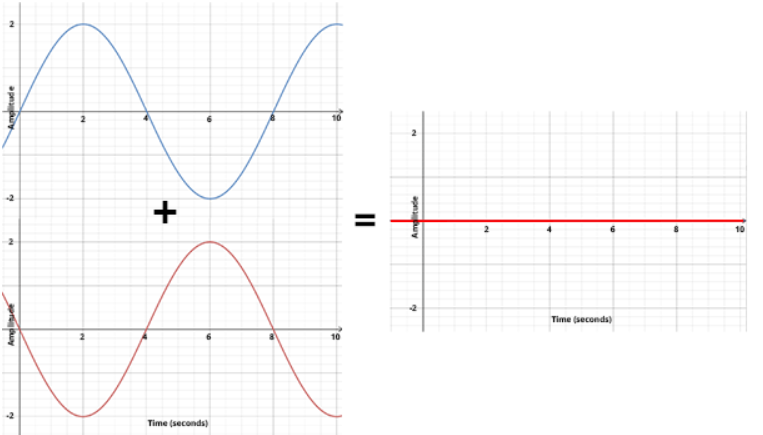
\includegraphics[width=10cm]{imagini/soundWaveCanceledAmplitude.png}
		\caption{Dou\u{a} unde sonore ,,defazate"}
		\label{Fig8}
	\end{figure}

	Diferen\c{t}a de faz\u{a} este exprimat\u{a} ca un unghi, deoarece forma de und\u{a} a unui ton pur alc\u{a}tuit\u{a} dintr-o singur\u{a} frecven\c{t}\u{a} poate fi descris\u{a} utiliz\^{a}nd func\c{t}ia sinus trigonometric\u{a}.	 
	
	Cele mai multe sunete sunt mult mai complexe dec\^{a}t o singur\u{a} frecven\c{t}\u{a}, dar constau \^{i}n schimb din multe unde sinusoidale diferite la frecven\c{t}e și amplitudini diferite. C\^{a}nd mai multe unde sinusoidale se combin\u{a} pentru a crea un sunet, formele de und\u{a} ale tuturor undelor sinusoidale sunt ad\u{a}ugate la fiecare loca\c{t}ie de-a lungul formei de und\u{a}.
	 	
	{\it{Energia (W)}} poate fi auzit\u{a} de fiin\c{t}ele vii. Sunetul este o und\u{a} mecanic\u{a} \c{s}i ca atare const\u{a} fizic \^{i}n compresie elastic\u{a} oscilatorie \c{s}i \^{i}n deplasarea oscilatorie a unui fluid. Prin urmare, mediul ac\c{t}ioneaz\u{a} ca stocare at\^{a}t pentru energia poten\c{t}ial\u{a}, c\^{a}t \c{s}i pentru energia cinetic\u{a}. \^{I}n consecin\c{t}\u{a}, energia sonor\u{a} dintr-un volum de interes este definit\u{a} ca suma densit\u{a}\c{t}ilor de energie poten\c{t}ial\u{a} \c{s}i cinetic\u{a}:
	
	\begin{equation}
	W = W_{\text{poten\c{t}ial\u{a}}} + W_{\text{cinetic\u{a}}}
	\end{equation}  
	
	{\it{Presiunea acustic\u{a}}} este abaterea presiunii locale fa\c{t}\u{a} de presiunea atmosferic\u{a}. \^{I}n aer, presiunea poate fi m\u{a}surat\u{a} cu ajutorul unui microfon, iar \^{i}n ap\u{a} cu ajutorul unui hidrofon. Unitatea de m\u{a}sur\u{a} dat\u{a} de c\u{a}tre Sistemul Interna\c{t}ional de Unit\u{a}\c{t}i de M\u{a}sur\u{a}, SI, pentru presiunea acustic\u{a} este Pascal (Pa). Formula folosit\u{a} pentru transformarea intensit\u{a}\c{t}ii \^{i}n presiune este:
	
	\begin{equation}
	p = \sqrt{2 I \rho c}, 
	\end{equation}
	
	\noindent unde $\rho$ este densitatea aerului, iar $c$ este viteza sunetului prin aer, iar $I$ este instensitatea.	 
	
	{\it{Puterea sunetului}} este rata la care energia sonor\u{a} este emis\u{a}, reflectat\u{a}, transmis\u{a} sau recep\c{t}ionat\u{a}, pe unitate de timp. Unitatea SI pentru puterea sunetului este Watt-ul (W). Pentru o surs\u{a} de sunet, spre deosebire de presiunea sonor\u{a}, puterea nu este dependent\u{a} nici de \^{i}nc\u{a}pere, nici de distan\c{t}\u{a}. Presiunea sonor\u{a} este o proprietate a c\^{a}mpului \^{i}ntr-un punct din spa\c{t}iu, \^{i}n timp ce puterea sonor\u{a} este proprietatea unei surse sonore, egal\u{a} cu puterea total\u{a} emis\u{a} de acea surs\u{a} \^{i}n toate direc\c{t}iile.
	 	
	{\it{Intensitatea (I)}} este definit\u{a} ca putere pe unitate de suprafa\c{t}\u{a} purtat\u{a} de o und\u{a}. {\it{Puterea (P)}} este rata la care energia este transferat\u{a} de und\u{a}. Unitatea de m\u{a}sur\u{a} folosi\u{a} pentru intensitate este $\dfrac{W}{m^2}$, iar formula acesteia este:
	
	\begin{equation}
	I=\frac{P}{A}
	\end{equation}
	 	
	Intensitatea sunetului este măsurată și raportată în decibeli (dB), o unitate care exprimă magnitudinea relativă a unui sunet pe o scară logaritmică. {\it{Nivelurile de intensitate}} ale sunetului sunt citate în decibeli (dB). Modul în care urechile noastre percep sunetul poate fi descris mai exact prin logaritmul intensit\u{a}\c{t}ii. Nivelul de intensitate ($\beta$) este definit astfel:
	
	\begin{equation}
	\beta(dB) = 10 \lg\left(\dfrac{I}{I_0}\right) 
	\end{equation}

	Omul de știință folosește, în mod obișnuit, patru termeni pentru a descrie amploarea unei unde sonore, fiecare dintre acestea putând fi tradus într-o versiune echivalentă a celeilalte. Amplitudinea se concentrează pe dimensiunea vibrației particulelor, iar presiunea sonoră asupra forței pe care o astfel de vibrație o exercită asupra mediului înconjurător. Ceilalți doi termeni, intensitate și putere, pun accentul pe noțiunea mai abstractă a energiei undei, corelând-o astfel cu alte forme de transfer și schimb de energie.
	
	Una dintre caracteristicile fizice importante legate de propagarea sunetului este impedanță acustică a mediului în care se deplasează unda sonoră. \textit{Impedanța acustică} este dată de raportul dintre presiunea acustică a undei și viteza sa de volum.
	
	\section{Reflexia sunetului}
	
	Principiile reflexiei pot fi aplicate undelor sonore, care constau din compresii \c{s}i refrac\c{t}ii. Dac\u{a} o und\u{a} sonor\u{a} se deplaseaz\u{a} printr-un tub cilindric, \^{i}n cele din urm\u{a} sunetul va ajunge la cap\u{a}tul tubului, acesta reprezent\^{a}nd grani\c{t}a dintre aerul din tub \c{s}i aerul din afara tubului. La atingerea cap\u{a}tului tubului, unda sonor\u{a} va suferi o reflec\c{t}ie par\c{t}ial\u{a} (o parte din energia transportat\u{a} va r\u{a}m\^{a}ne \^{i}n tub \c{s}i se va deplasa \^{i}n direc\c{t}ia opus\u{a}) \c{s}i o transmisie par\c{t}ial\u{a} (o parte din energia transportat\u{a} va trece peste grani\c{t}\u{a}, \^{i}n afara tubului).
	 
	
	Reflexia pe suprafe\c{t}e poate duce la unul dintre urm\u{a}toarele fenomene: ecou sau reverbera\c{t}ie. {\it{Ecoul}} este o reflexie a sunetului care ajunge la ascult\u{a}tor cu o \^{i}nt\^{a}rziere fa\c{t}\u{a} de sunetul direct. Aceast\u{a} \^{i}nt\^{a}rziere este direct propor\c{t}ional\u{a} cu distan\c{t}a suprafe\c{t}ei reflectate de la surs\u{a} la ascult\u{a}tor. Undele acustice sunt reflectate de pere\c{t}i sau de alte suprafe\c{t}e dure, cum ar fi mun\c{t}ii. Ecoul poate fi auzit atunci c\^{a}nd reflexia revine cu o amplitudine \c{s}i o \^{i}nt\^{a}rziere suficient\u{a} pentru a fi perceput\u{a} distinct. 
	 
	
	{\it{Reverberația}} reprezint\u{a} o persisten\c{t}\u{a} a sunetului dup\u{a} ce acesta a fost produs. O reverbera\c{t}ie este creat\u{a} atunci c\^{a}nd un sunet sau semnal provoac\u{a} multiple reflexii care se acumuleaz\u{a} \c{s}i apoi se descompun pe m\u{a}sur\u{a} ce sunetul este absorbit de suprafe\c{t}e. \^{I}n Figura \ref{Fig2}, observ\u{a}m dou\u{a} diagrame ce prezintă pe axa Ox, timpul, \c{s}i pe axa Oy, SPL (Sound Pressure Level) ce ilustreaz\u{a} diferen\c{t}a dintre ecou \c{s}i reverbera\c{t}ie. 
	
	\begin{figure}[!htb]
		\centering
		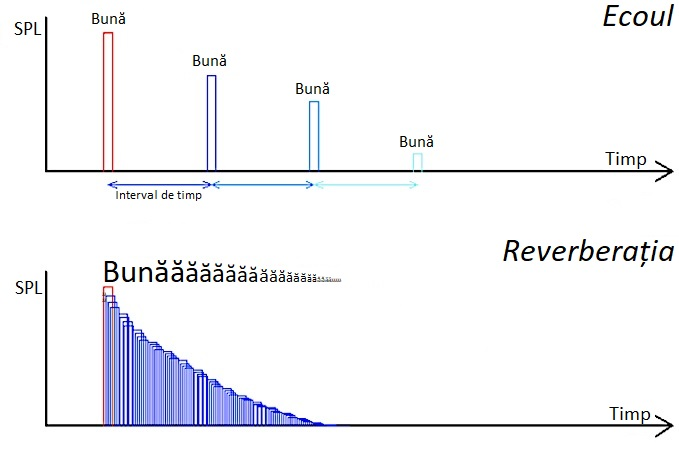
\includegraphics[width=1\linewidth]{imagini/EchoReverberation.jpg}
		\caption{Diferen\c{t}a dintre ecou \c{s}i reverbera\c{t}ie}
		\label{Fig2}
	\end{figure}

	Trasarea razelor pentru calcularea unghiurilor de inciden\c{t}\u{a} sau refrac\c{t}ie este dat\u{a} de legea lui Snell prin Ecua\c{t}ia \eqref{SnellEq} (vezi \cite{snell}):
	
	\begin{equation}
		\label{SnellEq}
		\frac{\sin \theta_2}{\sin \theta_1} = \frac{v_2}{v_1} = \frac{n_1}{n_2}
	\end{equation}

	\noindent unde $\theta_1, \theta_2$ sunt unghiurile de refrac\c{t}ie, $v_1, v_2$ reprezint\u{a} viteza de propagare prin mediu, iar $n_1, n_2$ sunt indicii de refrac\c{t}ie din mediu.
	
	\begin{figure}[!htb]
		\centering
		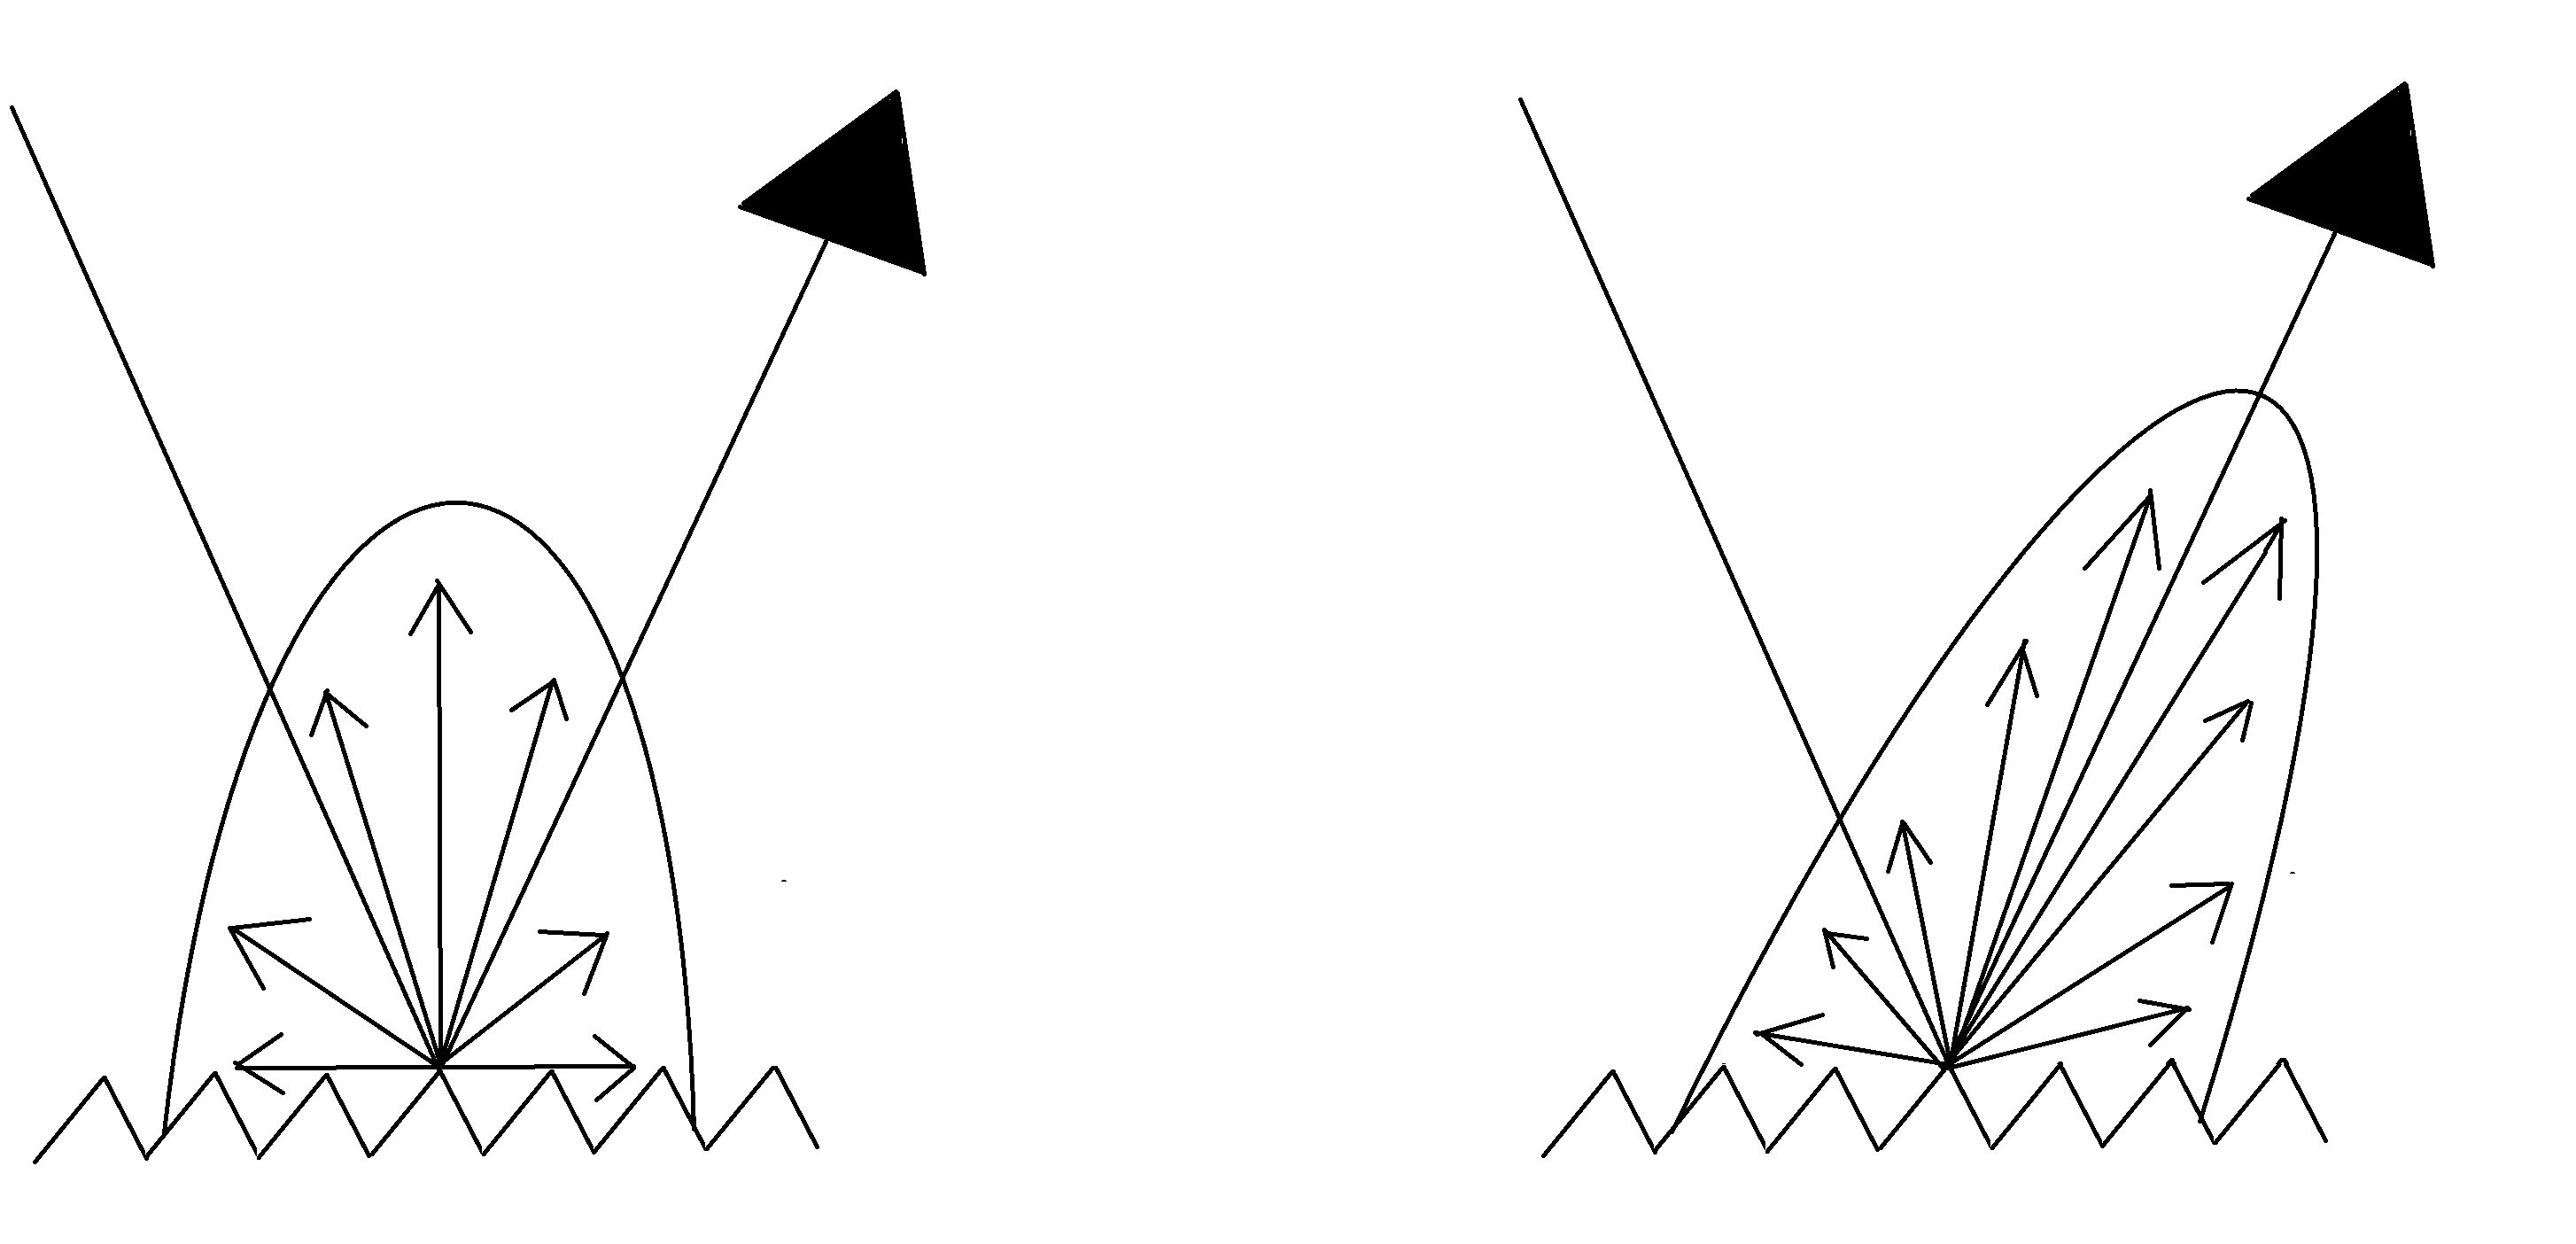
\includegraphics[width=0.7\linewidth]{imagini/reflections.png}
		\caption{Reflexie difuz\u{a} prin randomizare normal\u{a} \c{s}i reflexie difuz\u{a} prin randomizare ponderat\u{a}}
		\label{Fig10}
	\end{figure}

	Reflexiile sunetului pe suprafe\c{t}e nu urmeaz\u{a} \^{i}ntotdeauna legile lui Snell. Astfel, nici o reflexie nu este perfect specular\u{a}, deci este par\c{t}ial difuz\u{a}, iar acest lucru se \^{i}nt\^{a}mpl\u{a} ca o consecin\c{t}\u{a} pentru duritatea \c{s}i dimensiunea suprafe\c{t}ei de coliziune. Când o rază întâlnește o
	suprafață difuză, se generează un număr aleatoriu în intervalul [0, 1]. Dac\u{a} num\u{a}rul este mai mic dec\^{a}t un prag ales direc\c{t}ia razei este randomizat\u{a} pentru a simula difuzia, altfel	reflexia este specular\u{a}. Acest fenomen poate fi eviden\c{t}iat prin Figura \ref{Fig10}. \^{I}n aceast\u{a} lucrare se va folosi reflexia difuz\u{a} prin randomizare normal\u{a}.
	


	\section{Difrac\c{t}ia \c{s}i interferen\c{t}a sunetului}
	
	Difrac\c{t}ia reprezint\u{a} schimbarea local\u{a} \^{i}n direc\c{t}ia propag\u{a}rii undelor sonore trec\^{a}nd de marginea unui obstacol. Acesta este unul dintre cele mai importante fenomene acustice cauzat de natura sunetului, fiind una dintre cele mai complexe probleme de rezolvat. Efectele difrac\c{t}iei pot fi \^{i}mp\u{a}r\c{t}ite \^{i}n trei grupe: barier\u{a}, margine \c{s}i deschidere.
	 
	
	Fenomenul de difrac\c{t}ie depinde semnificativ de raportul dintre lungimea de und\u{a} a sunetului si m\u{a}rimea obstacolului. Cu c\^{a}t lungimea de und\u{a} este mai mare, cu at\^{a}t sunetul se intensific\u{a}. C\^{a}nd o und\u{a} sonor\u{a} \^{i}nt\^{a}lne\c{s}te un obstacol, care este mic \^{i}n raport cu lungimea de und\u{a}, valul trece \^{i}n jurul ei ca \c{s}i c\^{a}nd nu ar exista, form\^{a}nd foarte pu\c{t}in\u{a} umbr\u{a}. Dac\u{a} frecven\c{t}a sunetului este suficient de mare, lungimea de und\u{a} este suficient de scurt\u{a} \c{s}i ca urmare se formeaz\u{a} o umbr\u{a} vizibil\u{a}.
	 
	
	\^{I}n Figura \ref{Fig3} se pot observa cele trei tipuri de difrac\c{t}ii, unde situa\c{t}iile din partea de sus sunt ideale pentru frecven\c{t}ele joase, iar cazurile din partea de jos sunt de dorit pentru frecven\c{t}ele \^{i}nalte.
	 
	
	\begin{figure}[!htb]
		\centering
		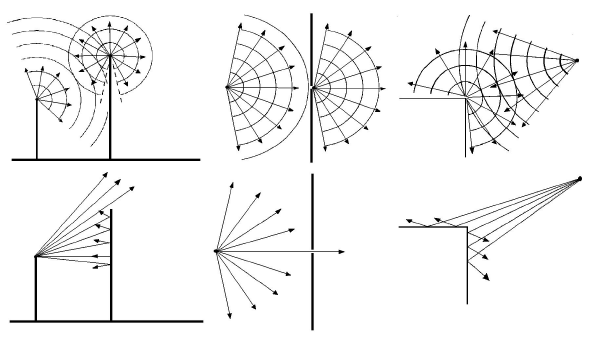
\includegraphics[width=0.8\linewidth]{imagini/difractie.png}
		\caption{Difrac\c{t}ie barier\u{a}, deschidere, margine\cite{elorza}}
		\label{Fig3}
	\end{figure}
	
	Dou\u{a} unde care c\u{a}l\u{a}toresc \^{i}n acela\c{s}i mediu vor interfera una cu cealalt\u{a}. Dac\u{a} amplitudinile lor se adun\u{a}, se spune c\u{a} aceasta este o interferen\c{t}\u{a} constructiv\u{a} și se află ,,în fază''. O interferen\c{t}\u{a} distructiv\u{a} se constituie din două unde ,,defazate'' și se realizeaz\u{a} atunci c\^{a}nd cele dou\u{a} unde sonore sunt defazate \c{s}i scad. Interferența constructivă duce la o creștere a amplitudinii undei, în timp ce interferența distructivă poate duce la anularea totală a undelor care contribuie.
	 
	Difracția sunetului este utilă în cazul sistemelor audio, în care sunetul provenit de la difuzoare se răspândește și se reflectă de pe pereți pentru a umple o cameră. Pe de altă parte, capacitatea unei unde sonore de a se difracta scade pe măsură ce frecvența crește și lungimea de undă se micșorează. De asemenea, deoarece lungimile de undă ale semnalelor ultrasonice devin extrem de mici la frecvențe înalte, este posibil să se creeze un fascicul de ultrasunete. Fasciculele cu ultrasunete au devenit foarte utile în medicina modernă.
	
	\^{I}n acest studiu, difrac\c{t}ia nu va fi un subiect abordat.
	
	\section{Func\c{t}ia de r\u{a}spuns la impuls}
	
	Propagarea sunetului de la o surs\u{a} audio la un receptor se caracterizeaz\u{a} prin func\c{t}ia de r\u{a}spuns impuls \c{s}i informa\c{t}iile spa\c{t}iale pe toate c\u{a}ile de propagare posibile. Prima detectare corespunde \^{i}ntotdeauna cu sunetul direct \c{s}i, dup\u{a} aceasta, primesc reflexii multiple. \^{I}nt\^{a}rzierile lor de timp \^{i}n ceea ce prive\c{s}te sunetul direct sunt \^{i}n func\c{t}ie de lungimile c\u{a}ilor parcurse \c{s}i intensit\u{a}\c{t}ile lor de presiune depind de absorb\c{t}ia sunetului prin aer, precum \c{s}i de caracteristicile de absorb\c{t}ie a suprafe\c{t}elor implicate \^{i}n fiecare cale.
	 
	
	R\u{a}spunsul la impuls este func\c{t}ia de ie\c{s}ire a unui sistem dinamic atunci c\^{a}nd la intrare se aplic\u{a} o func\c{t}ie unitar\u{a} (func\c{t}ia Delta Dirac). Un impuls este un eveniment sonor foarte puternic \c{s}i scurt, care este utilizat pentru testarea r\u{a}spunsului la sunet \^{i}ntr-o camer\u{a} sau pentru a testa eficien\c{t}a unui sistem acustic. Un impuls con\c{t}ine toate frecven\c{t}ele.
	  
	În matematică, funcția Delta Dirac este o funcție generalizată sau o distribuție introdusă de fizicianul Paul Dirac. În inginerie și în procesarea de semnale, funcția Delta, cunoscută și sub numele de simbol al impulsului de unitate, poate fi privită prin transformarea sa Laplace, ca provenind de la valorile limită ale unei funcții analitice complexe a unei variabile complexe. Convoluția unui semnal cu delta Dirac poate fi gândită ca o stimulare, care include toate frecvențele. Acest lucru duce la o rezonanță cu semnalul, făcând semnalul teoretic „real”. Regulile formale respectate de această funcție fac parte din calculul operațional, un set de instrumente standard de fizică și inginerie. În multe aplicații, Delta Dirac este privită ca un fel de limită a unei funcții de impuls.
	
	Delta Dirac este utilizată pentru a modela o funcție de impuls și alte abstracții similare, cum ar fi o sarcină punctuală, o masă punctuală sau un punct electronic. De exemplu, pentru a calcula dinamica unei mingi de biliard lovite, se poate aproxima forța impactului cu o funcție Delta. Procedând astfel, nu numai că simplificăm ecuațiile, dar putem calcula și mișcarea mingii luând în considerare doar impulsul total al coliziunii fără un model detaliat al întregului transfer de energie elastică la niveluri subatomice.
	
	O func\c{t}ie de r\u{a}spuns la impuls se compune din: sunet direct, prima \^{i}nt\^{a}rziere, reflec\c{t}ii timpurii \c{s}i coada reverberant\u{a}. Figura \ref{Fig4} ilustreaz\u{a} componentele unei func\c{t}ii de r\u{a}spuns la impuls.
	
	\begin{figure}[!htb]
		\centering
		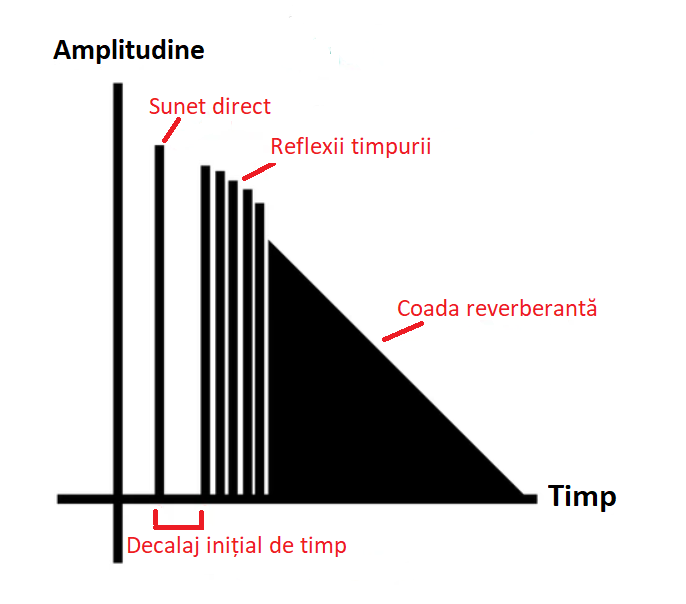
\includegraphics[width=0.7\linewidth]{imagini/impulseResponse.png}
		\caption{Func\c{t}ia de r\u{a}spuns la impuls}
		\label{Fig4}
	\end{figure}

	{\it{Sunetul direct (Direct Sound)}} are presiunea acustic\u{a} ridicat\u{a}, dar durat\u{a} scurt\u{a}, reprezent\^{a}nd timpul necesar pentru ca sunetul s\u{a} ajung\u{a} la cel primit (ex: ascult\u{a}tor sau microfon).
	 
	
	{\it{Decalaj ini\c{t}ial de timp (Initial Time Delay Gap)}}	reprezint\u{a} timpul dintre sunetul direct \c{s}i primele reflexii \c{s}i ne spune c\^{a}t de departe este sursa de sunet. Cu c\^{a}t decalajul ini\c{t}ial de timp este mai lung, cu at\^{a}t este mai apropiat\u{a} sursa de sunet. Cu alte cuvinte, dac\u{a} sursa este departe, sunetul direct \c{s}i primele reflexii se vor auzi ca și cum ar fi mai apropiate.
	 
	
	{\it{Reflexii timpurii (First Order Reflections sau Early Reflections)}} sunt primele pe care le auzim \c{s}i se disting. Este posibil s\u{a} fie doar c\^{a}teva \^{i}ntr-o camer\u{a} simpl\u{a} dreptunghiular\u{a}, dar pot fi mai multe dac\u{a} camera este mai complex\u{a}. Reflexiile timpurii indic\u{a} c\^{a}t de mare este o camer\u{a}.
	 
	
	{\it{Coada reverberant\u{a}}} const\u{a} \^{i}n reflexii de ordin superior \c{s}i nu se pot distinge \^{i}ntre ele. Pe m\u{a}sur\u{a} ce num\u{a}rul de reflexii cre\c{s}te, undele sonore pierd energie \c{s}i, \^{i}n cele din urm\u{a}, se descompun. Dezintegrarea reverberant\u{a} este adesea liniar\u{a} atunci c\^{a}nd este reprezentat\u{a} grafic ca mai sus. 
	
	\section{Func\c{t}ia de r\u{a}spuns în frecven\c{t}\u{a}}
	
	Gama spectrului audio se întinde de la 20 Hz la 20.000 Hz și poate fi împărțită eficient în șapte benzi de frecvență diferite, fiecare bandă având un impact diferit asupra sunetului total. Sub-basul, cuprinde intervalul de la 20 la 60 Hz, oferă primele frecvențe joase utilizabile pe majoritatea înregistrărilor. Basul profund produs în această gamă se simte, de obicei, mai mult decât se aude, oferind un sentiment de putere. Multe instrumente se luptă să intre în acest interval de frecvență, cu excepția câtorva instrumente cu bas greu, cum ar fi chitara basă care are cel mai mic ton realizabil de 41 Hz. Este dificil de auzit gama sub-basului la volume mici datorită curbei Fletcher Munson, un contur cu intensitate egală care reprezintă o măsură a nivelului de presiune acustică, peste spectrul de frecvență, pentru care un ascultător percepe o intensitate constantă atunci când este prezentat cu tonuri stabile pure.
	
	Basul este cea de-a doua gamă și cuprinde intervalul de la 60 la 250 Hz. Notele fundamentale ale ritmului sunt centrate pe această zonă. Cele mai multe semnale de bas în piesele de muzică modernă se află în jurul zonei de 90-200 Hz. Frecvențele în jurul valorii de 250 Hz pot adăuga o senzație de căldură la bas fără pierderea definiției.
	
	Gama medie joasă conține armonicele de ordin scăzut ale majorității instrumentelor și este în general privită ca gama de prezență a basului și cuprinde valorile din intervalul 250-500 Hz. Creșterea semnalului în jurul valorii de 300 Hz adaugă claritate instrumentelor de bas și corzilor inferioare. Creșterea prea mare în jurul valorii de 500 Hz poate face ca instrumentele cu frecvență mai mare să pară înăbușite.
	
	Intervalul mediu, 500 Hz - 2kHz, determină cât de proeminent este un instrument în mix. Creșterea în jur de 1000 Hz poate conferi instrumentelor o calitate asemănătoare claxonului. Excesul de ieșire la acest interval poate suna subțire și poate provoca oboseală a urechii. Dacă creșteți în acest domeniu, fiți foarte precauți, mai ales la voce. Urechea este deosebit de sensibilă la modul în care sună vocea umană și la acoperirea frecvenței acesteia.
	
	Auzul uman este extrem de sensibil la frecvențele medii ridicate, cuprinse  în intervalul 2-4kHz, cu cel mai mic impuls aici rezultând o schimbare imensă a timbrului sunetului. Gama medie înaltă este responsabilă pentru atacul asupra instrumentelor percutante și ritmice. Dacă este amplificat, acest interval poate adăuga prezență. Cu toate acestea, o creștere prea mare în jurul gamei de 3 kHz poate provoca oboseală la ascultare.
	
	Gama de prezență, 4-6 kHz, este responsabilă pentru claritatea și definirea unui sunet. Este intervalul în care majoritatea aparatelor stereo de acasă își centrează înaltele. Suprasolicitarea poate provoca un sunet iritant și dur. Tăierea în această gamă face ca sunetul să fie mai îndepărtat și mai transparent.
	
	Gama de strălucire, 6-20 kHz, este compusă în întregime din armonici și este responsabilă pentru strălucirea și aerul unui sunet. Creșterea în jurul valorii de 12 kHz face ca sunetul de înregistrare să devină mai Hi-Fi. Hi-Fi(High Fidelity) este un termen folosit de ascultători, audiofili și pasionați de sunet acasă pentru a se referi la reproducerea sunetului de înaltă calitate.

	Frecvențele mai mici de 20 Hz se numesc infrasunete, iar frecvențele care sunt mai mari de 20 kHz se numesc ultrasunete. Infrasunetele pot fi auzite și folosite de animale precum: elefanții și balenele, iar ultrasunetele sunt, de obicei, folosite în domeniul medical.
	
	\begin{figure}[!htb]
		\centering
		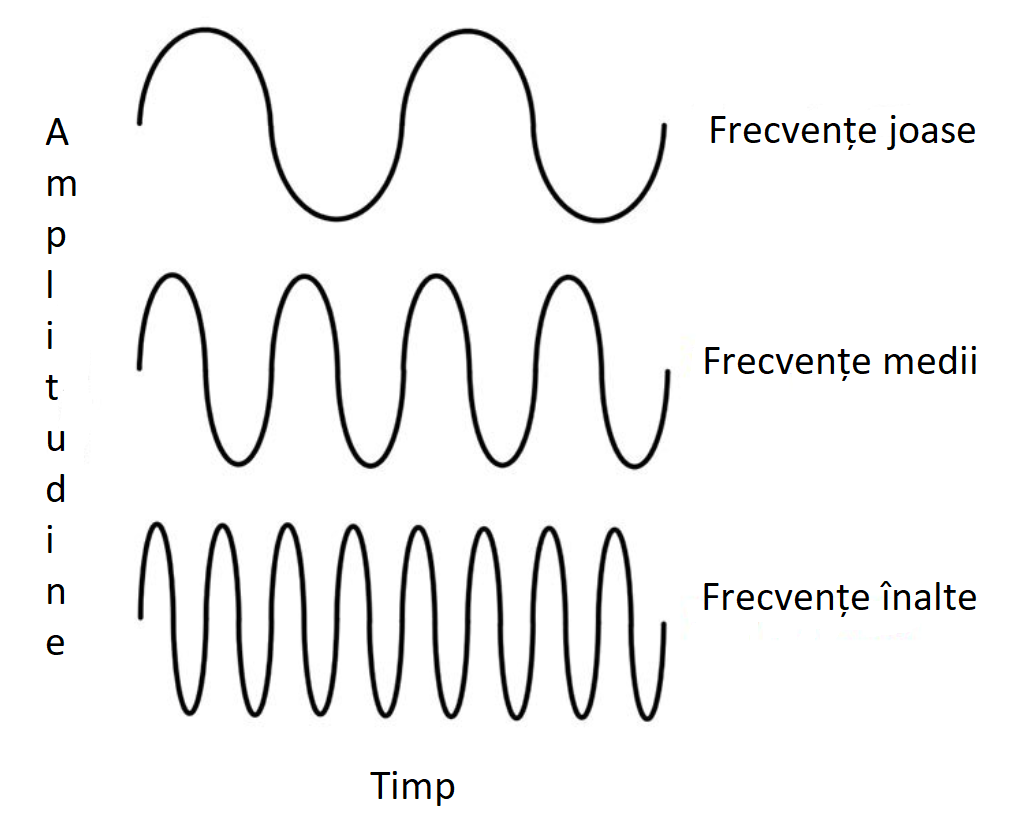
\includegraphics[width=12cm]{imagini/ampli_timp.png}
		\caption{Tipuri de frecvențe}
		\label{Fig30}
	\end{figure}

	Dacă urmăurim undele sinusoidale din Figura \ref{Fig30} putem observa că pe măsură ce crește frecvența, perioada de timp pentru un ciclu devine progresiv mai scurtă, astfel încât în comparație cu o singură perioadă de timp de $360^\circ$ la frecvență joasă, o perioadă de timp cu frecvență înaltă poate include 2 sau mai multe cicluri în aceeași perioadă de timp ca o frecvență mai mică. Astfel, avem ilustrate frecvențele joase, medii și înalte în funcție de amplitudine și timp.
	
	Răspunsul în frecvență este măsura cantitativă a spectrului de ieșire al unui sistem sau dispozitiv ca răspuns la un stimul și este utilizat pentru a caracteriza dinamica sistemului. Este o măsură a magnitudinii și a fazei în funcție de frecvență, în comparație cu intrarea. În termeni simpli, dacă o undă sinusoidală este injectată într-un sistem la o frecvență dată, un sistem liniar va răspunde la aceeași frecvență cu o anumită magnitudine și un anumit unghi de fază relativ la intrare.	 
	
	\^{I}n contextul unui sistem audio, obiectivul poate fi reproducerea semnalului de intrare f\u{a}r\u{a} distorsiuni. Acest lucru necesit\u{a} o amplitudine de r\u{a}spuns uniform p\^{a}n\u{a} la limitarea l\u{a}\c{t}imii de band\u{a} a sistemului, cu semnalul \^{i}nt\^{a}rziat cu exact aceea\c{s}i cantitate de timp la toate frecven\c{t}ele.	 
	
	Estimarea r\u{a}spunsului \^{i}n frecven\c{t}\u{a} pentru un sistem fizic implic\u{a}, \^{i}n general, excitarea semnalului cu un semnal de intrare, m\u{a}surarea istoricelor de timp de intrare \c{s}i de ie\c{s}ire \c{s}i compararea celor dou\u{a} printr-un proces precum Transformarea Fourier Rapid\u{a} (FFT).
	
	R\u{a}spunsul \^{i}n frecven\c{t}\u{a} se caracterizeaz\u{a} prin amploarea r\u{a}spunsului sistemului, m\u{a}sur\-at\u{a}, de obicei, \^{i}n decibeli (dB), \c{s}i faza, m\u{a}surat\u{a} \^{i}n radiani sau grade. Funcția de răspunsul în frecvență are, în general, valori complexe, cu părți reale și imaginare. Acest lucru este adesea mai util și mai intuitiv atunci când este exprimat în coordonate polare. Adică îl putem separa în magnitudinea sa (numită răspuns de amplitudine) și în componentă de fază (numită răspuns de fază).
	
	Fiecare componentă din semnal ar trebui să aibă, în mod ideal, un răspuns de frecvență plat, astfel încât sunetul să treacă nealterat. Dar realitatea este că multe componente nu oferă performanțe ideale. Un răspuns neliniar va modifica modul în care sună sursa noastră. Cu toate acestea, nu este vorba doar de concepte obișnuite, cum ar fi basul și înalte, ci afectează și calitatea sunetului fiecărui instrument din mix. Pentru a ne pune capul în jurul acestui aspect mai subtil al modului în care răspunsul de frecvență neliniar poate afecta ceea ce auzim, trebuie să apelăm la analiza Fourier.
	
	\section{Absorb\c{t}ia sunetului}
	
	\^{I}n contextul propag\u{a}rii sunetului \^{i}n spa\c{t}ii \^{i}nchise vom considera dou\u{a} tipuri de absorb\c{t}ii: \textit{absorb\c{t}ia aerului} \c{s}i \textit{absorb\c{t}ia suprafe\c{t}elor}.
	 
	
	\textit{Coeficientul de absorb\c{t}ie \^{i}n aer}, depinde de temperatura atmosferic\u{a}, de presiunea atmosferic\u{a} \c{s}i de frecven\c{t}\u{a}. Absorb\c{t}ia sunetului \^{i}n acustic\u{a} este cauzat\u{a} de caracteristicile de absorb\c{t}ie ale suprafe\c{t}elor. Atunci când ținem cont de absorbția aerului putem îmbunătății rezultatele pentru încăperile de dimensiuni mari sau atunci când considerăm frecvențe înalte.
	
	Astfel, absorb\c{t}ia este definit\u{a} ca o disipare a energiei sonore la lovirea unei suprafe\c{t}e fizice. La fiecare reflexie, o parte $\alpha$ din energia sau puterea sa este absorbit\u{a}. Acest factor $\alpha$ se nume\c{s}te coeficient de absorb\c{t}ie. Absorb\c{t}ia sunetului depinde de unghiul de inciden\c{t}\u{a}.
	
	În solide și lichide se absoarbe mai puțin sunet decât în gaze, sunetele se pot propaga pe distanțe mult mai mari în aceste medii. De exemplu, marea gamă pe care pot comunica anumite mamifere marine este posibilă parțial prin atenuarea redusă a sunetului în apă. În plus, deoarece absorbția crește odată cu frecvența, devine foarte dificil ca undele ultrasonice să pătrundă într-un mediu dens. Aceasta este o limitare persistentă a dezvoltării aplicațiilor cu ultrasunete de înaltă frecvență.
	
	Un alt mecanism de absorb\c{t}ie a sunetului este \textit{absorb\c{t}ia suprafe\c{t}elor}, fiind definit ca disiparea energiei sonore la lovirea unei suprafe\c{t}e fizice. La fiecare reflexie, o parte din energie sau putere este absorbit\u{a}. Restul de energie care nu este absorbit\u{a} este fie absorbit\u{a} de material, fie transmis\u{a} mai departe ca sunet reflectat. Formula utilizat\u{a} \^{i}n aceast\u{a} lucrare este eviden\c{t}iat\u{a} prin Ecuatia \eqref{ecuatia3}.
	
	\begin{equation}
		W = W(1-\alpha)
		\label{ecuatia3}
	\end{equation}
	
	\noindent unde $W$ este energia.
	
	Absorbția sunetului nedorit, precum cel al mașinilor din fabrici, este esențială pentru sănătatea lucrătorilor, iar controlul zgomotului în acustica arhitecturală și industrială s-a extins pentru a deveni un domeniu important al ingineriei acusticii.
	
	Materialele de absorbție a sunetului sunt utilizate pe scară largă în multe aplicații de control al zgomotului. Comportamentul acustic al acestor materiale poate fi măsurat folosind tubul de impedanță cu eșantioane de dimensiuni mici, dar în practică, materialele utilizate în aplicațiile de control al zgomotului nu sunt mici, iar undele incidente de pe acestea nu sunt unde plane. În practică, materiale în diferite dimensiuni și forme sunt utilizate în aplicații de control al zgomotului, iar câmpul acustic este difuz. Impedanța acustică este o măsură a ușurinței cu care o undă sonoră se propagă printr-un anumit mediu.
	
	Coeficientul de absorbție reprezintă raportul dintre energia absorbită de suprafață și energia incidentă. Conform definiției sale, coeficientul de absorbție a sunetului unei suprafețe poate presupune valori cuprinse între 0 (suprafețe care reflectă total) și 1 (suprafețe absorbante total).
	
	Calitatea acustică a unei camere depinde de reverberație, care la rândul ei este direct proporțională cu volumul camerei și invers proporțională cu capacitatea de a absorbi sunetul materialelor limită și a tuturor celorlalte obiecte plasate în interiorul camerei.
	
	În această lucrare se va ține cont doar de coeficientul de absorbție al suprafețelor.
	
	\section{Simularea binaural\u{a}}
	
	\textit{Simularea binaural\u{a}} reprezint\u{a} o metod\u{a} de a realiza semnale binaurale la ambele urechi ale receptorului \^{i}n spa\c{t}ii inexistente prin intermediul unui model. \^{I}n ultima perioad\u{a}, simularea acustic\u{a} a devenit din ce \^{i}n ce mai important\u{a} pentru proiectarea spa\c{t}iilor \^{i}nchise, precum s\u{a}lile de concerte \c{s}i de teatru.
	 
	
	Exist\u{a} o mul\c{t}ime de tehnici de simulare binaural\u{a} \^{i}n combina\c{t}ie cu metode de calcul, de cele mai multe ori tehnici geometrice pentru calcul acustic, precum: metoda sursei de imagine \^{i}n oglind\u{a}, ray-tracing sau metode hibride. Cu toate acestea, genul acesta de tehnici vin la pachet cu cre\c{s}terea timpului de calcul. Unul dintre cele mai dificile lucruri este directivitatea sursei.
	
	 
	De\c{s}i este imposibil\u{a} simularea cu exactitate a unui c\^{a}mp sonor real folosind metode geometrice, lucr\u{a}rile realizate p\^{a}n\u{a} \^{i}n prezent pe aceste teme s-au bucurat de un mare succes, iar unele au fost chiar comercializate. O alt\u{a} provocare \^{i}n crearea unui astfel de algoritm este dat\u{a} de coada reverberant\u{a} datorit\u{a} efortului considerabil de timp. Simularea binaural\u{a} nu va fi tratat\u{a} \^{i}n acest studiu.
	
	\begin{figure}[!htb]
		\centering
		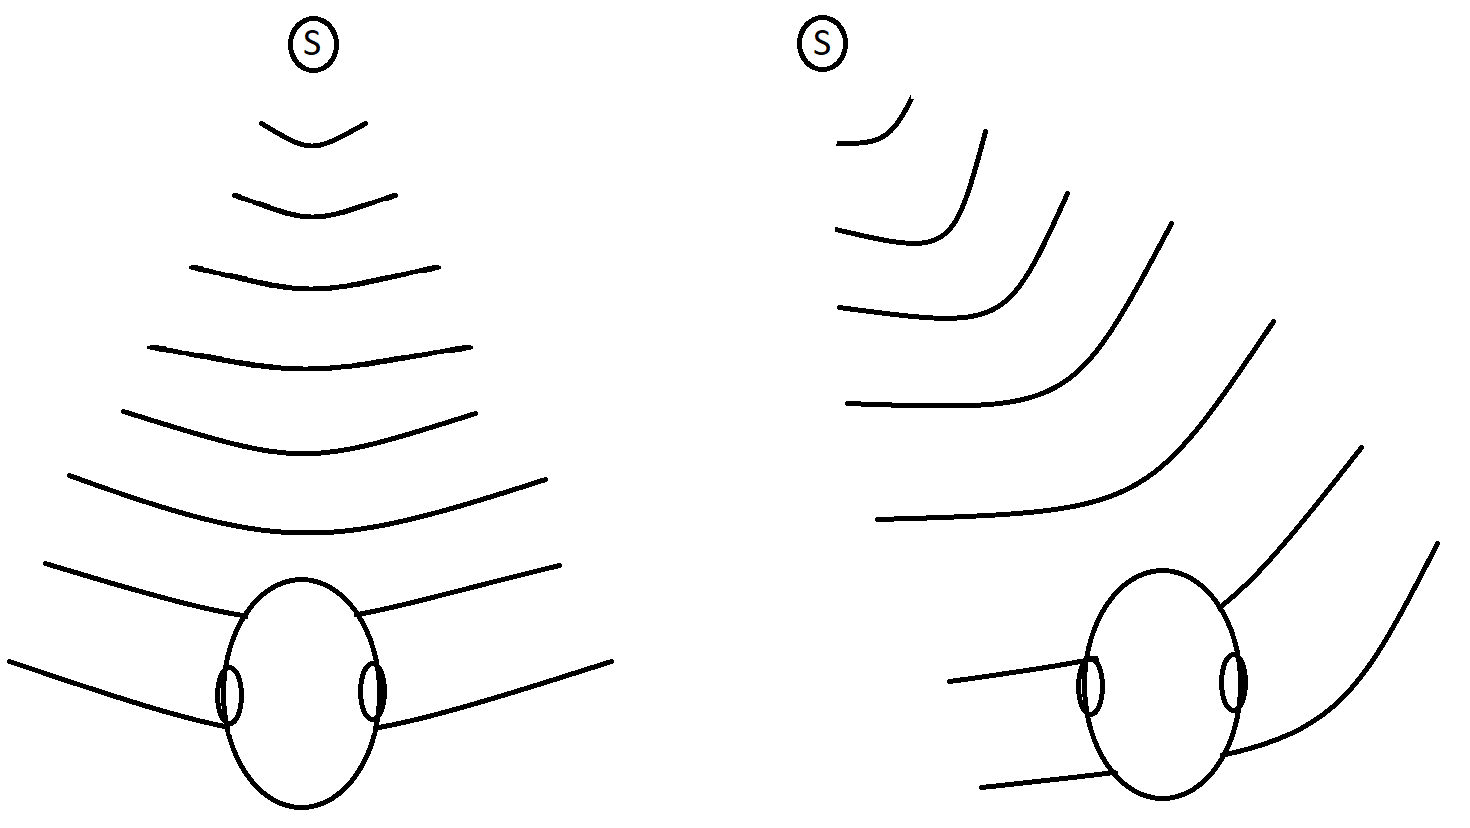
\includegraphics[width=1\linewidth]{imagini/binauralExample.png}
		\caption{Exemplu de simulare binaural\u{a}}
		\label{Fig12}
	\end{figure}

	\^{I}n Figura \ref{Fig12}, se poate observa beneficiul unei simul\u{a}ri binaurale. \^{I}n prima parte a figurii, sunetul ajunge de la surs\u{a} (S) la urechile omului \^{i}n acela\c{s}i moment \c{s}i cu aceea\c{s}i intensitate, pe c\^{a}nd \^{i}n partea din dreapta imaginii sunetul ajunge mai devreme la urechea st\^{a}ng\u{a} dec\^{a}t la urechea dreapt\u{a} \c{s}i la intensit\u{a}\c{t}i diferite. Urechea st\^{a}ng\u{a} va auzi mai puternic sunetul dec\^{a}t urechea dreapt\u{a}. 

	\section{Tehnica de trasare a razelor (Ray-Tracing)}
	
	Intensitatea emis\u{a} de o surs\u{a} este descris\u{a} de un num\u{a}r finit de raze, care vor fi considerate purt\u{a}tori de intensitate (sau de energie sau de putere). Aceste raze c\u{a}l\u{a}toresc prin spa\c{t}iu la viteza sunetului \c{s}i sunt reflectate dup\u{a} fiecare coliziune cu limitele camerei. \^{I}n acest timp, intensitatea lor scade ca o consecin\c{t}\u{a} a absorb\c{t}iei aerului \c{s}i a pere\c{t}ilor pe care raza \^{i}i intersecteaz\u{a}.
	 
	
	Dac\u{a} sursa sonor\u{a} are caracteristici omnidirec\c{t}ionale, direc\c{t}iile razelor sunt create prin distribu\c{t}ii aleatoare omogene. Calea posibil\u{a} pentru fiecare raz\u{a} emis\u{a} de la surs\u{a} trebuie gasit\u{a}. Raza este considerat\u{a} un vector care \^{i}\c{s}i schimb\u{a} direc\c{t}ia la fiecare reflexie, fiind astfel posibil\u{a} determinarea urm\u{a}toarei suprafe\c{t}e de ciocnire. 
	 
	
	De obicei, sursa este \^{i}mp\u{a}r\c{t}it\u{a} \^{i}ntr-un num\u{a}r mare de piese mici. Metoda determinist\u{a} este \^{i}mp\u{a}r\c{t}irea sursei \^{i}ntr-o manier\u{a} matematic\u{a} sau geometric\u{a}. Piesele din surs\u{a} ar trebui s\u{a} fie identice sau c\^{a}t de mult posibil identice. Punctele selectate aleatoriu pe suprafa\c{t}a unei sfere surs\u{a} pot fi reprezentate de trei parametrii: raza, azimutul \c{s}i eleva\c{t}ia \cite{jeong}. Mai mult dec\^{a}t a propus Jeong Cheol-Ho \^{i}n studiul s\u{a}u, \^{i}n aceast\u{a} lucrare \^{i}mp\u{a}r\c{t}irea sursei \^{i}n piese mai mici s-a realizat cu ajutorul sferei lui Fibonacci, algoritm ce urmeaz\u{a} s\u{a} fie descris \^{i}n capitolele urm\u{a}toare.
	 
	
	Mai departe, aceste puncte reprezint\u{a} pozi\c{t}ia de start pentru o raz\u{a}. Fiecare raz\u{a} poate avea nici una sau mai multe reflexii \c{s}i, astfel, s\u{a} fie considerat\u{a} o raz\u{a} direct\u{a} sau indirect\u{a}. Fiecare coliziune este re\c{t}inut\u{a} \c{s}i putem observa care a fost traseul pe care fiecare raz\u{a} l-a parcurs \^{i}n \^{i}nc\u{a}pere de la surs\u{a} p\^{a}n\u{a} la ascult\u{a}tor.
	 
	
	Intensitatea pe care o raz\u{a} o transmite receptorului este direct dependent\u{a} de distan\c{t}a pe care raza a parcurs-o \^{i}n \^{i}nc\u{a}pere. Intensitatea la un anumit moment se calculeaz\u{a} astfel dependent de absorb\c{t}ia aerului, de lungimea traseului parcurs \c{s}i de propriet\u{a}\c{t}ile de absorb\c{t}ie ale peretelui. Coliziunea cu suprafa\c{t}a poate fi considerat\u{a} specular\u{a}, conform legii lui Snell.	Tot acest proces trebuie repetat pentru fiecare frecven\c{t}\u{a}.
	 
	
	\^{I}n Figura \ref{Fig9} este ilustrat un mod de reprezentare pentru tehnica Ray-Tracing, unde se poate observa traiectul razelor. Linia continu\u{a} reprezint\u{a} raza direct\u{a}, iar liniile punctate semnific\u{a} razele indirecte.
	
	\begin{figure}[!htb]
		\centering
		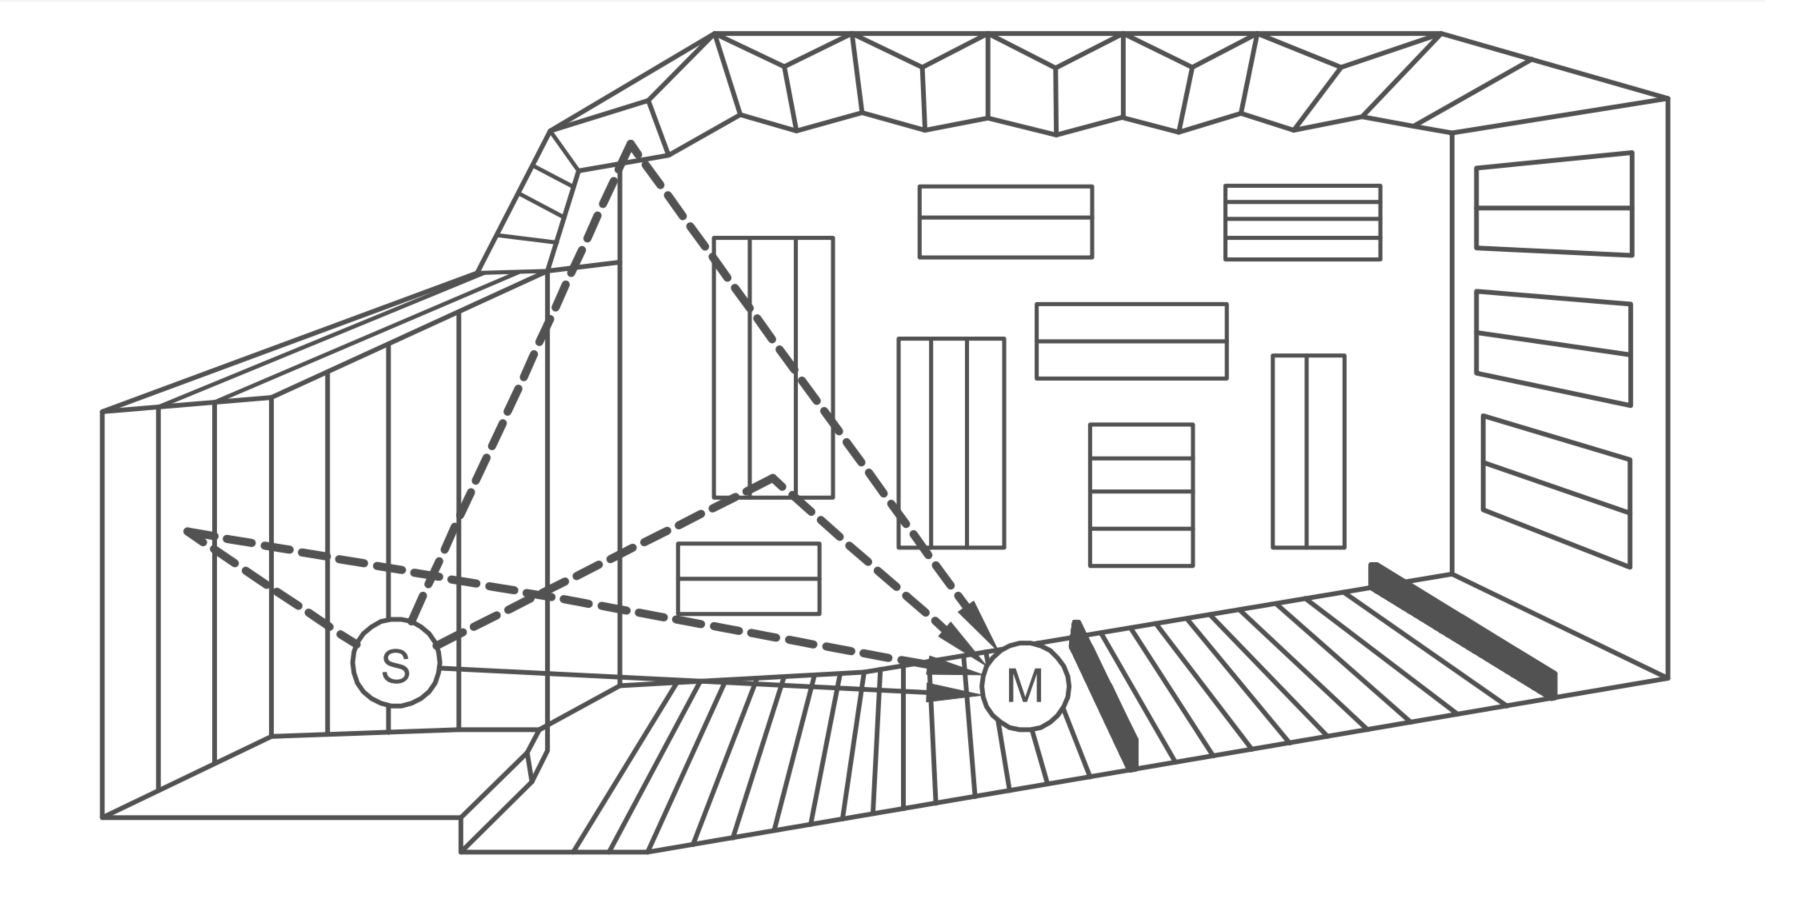
\includegraphics[width=1\linewidth]{imagini/roomExample.png}
		\caption{Exemplu de ray-tracing}
		\label{Fig9}
	\end{figure}
	
	S-a demonstrat c\u{a} algoritmul de Ray-Tracing prezice nivelurile de zgomot cu o precizie foarte bun\u{a} \c{s}i este considerat drept unul dintre cele mai elegante metode de reprezentare a reflexiilor. Cu toate acestea, exist\u{a} limit\u{a}ri, excep\c{t}ii \c{s}i probleme. Exist\u{a} c\^{a}teva elemente care ar trebui luate \^{i}n considerare atunci c\^{a}nd implement\u{a}m sau evalu\u{a}m un astfel de algoritm, precum: \textit{intervalul de frecven\c{t}e}, \textit{factori dependen\c{t}i de frecven\c{t}\u{a}}, \textit{geometria}, \textit{num\u{a}rul de raze}.
	 
	
	\^{I}n mod normal, singurii factori dependen\c{t}i de frecven\c{t}\u{a} care pot fi inclu\c{s}i sunt coeficien\c{t}ii de absorb\c{t}ie \c{s}i estimarea statistic\u{a} a propriet\u{a}\c{t}ilor difuze. O ipotez\u{a} de baz\u{a} \^{i}n metodele care utilizeaz\u{a} raze este c\u{a} lungimea de und\u{a} corespunz\u{a}toare celei mai mici frecven\c{t}e este mai mic\u{a} \^{i}n compara\c{t}ie cu dimensiunile camerei \c{s}i suprafe\c{t}ele acesteia.
	 
	
	Precum am men\c{t}ionat mai sus, coeficientul de absorb\c{t}ie $\alpha$ este dependent de unghi. Principalul motiv pentru evitarea m\u{a}sur\u{a}torilor dependente de unghi este c\u{a} acestea ar trebui s\u{a} fie foarte precise. Acest lucru fiind destul de dificil, \^{i}ntruc\^{a}t presupune stocarea tuturor materialelor de construc\c{t}ie. Prin urmare, a fost acceptat\u{a} estimarea caracteristicilor de absorb\c{t}ie a unei suprafe\c{t}e printr-o form\u{a} care este \^{i}n medie peste toate unghiurile de inciden\c{t}\u{a}.
	 
	
	Erori numerice sunt introduse \^{i}n rezultate prin utilizarea unui num\u{a}r limitat de raze, deoarece unghiul dintre raze adiacente r\u{a}m\^{a}ne constant, iar aceast\u{a} reprezentare devine treptat mai pu\c{t}in exact\u{a} odat\u{a} cu sc\u{a}derea num\u{a}rului de raze. Pentru a atinge criteriile de convergen\c{t}\u{a}, num\u{a}rul de raze trebuie s\u{a} fie c\^{a}t mai mare, cu c\^{a}t num\u{a}rul de raze este mai mare, cu at\^{a}t este mai mic unghiul solid pe care \^{i}l va acoperi o raz\u{a}. Acest lucru poate afecta timpul de calcul, dar \c{s}i un num\u{a}r prea mic de raze poate genera probleme. 
	 
	
	Pentru a putea \^{i}n\c{t}elege mai bine traiectul unei raze vom folosi Figura \ref{Fig11}. S \c{s}i M reprezint\u{a} sursa \c{s}i microfonul, iar linia trasat\u{a} este drumul parcurs de raz\u{a} p\^{a}n\u{a} la microfon, drum care presupune 4 reflexii speculare. Modelul de propagare al sunetului ce urmeaz\u{a} s\u{a} fie prezentat \^{i}n aceast\u{a} lucrare va folosi doar reflexii speculare.
	 
	
	\begin{figure}[!htb]
		\centering
		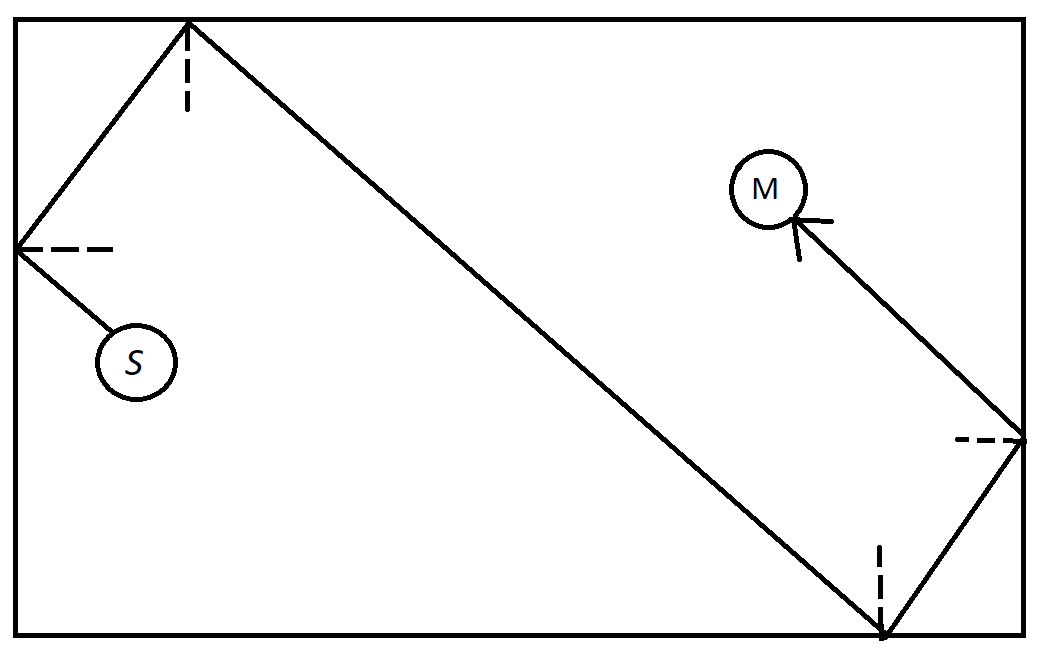
\includegraphics[width=1\linewidth]{imagini/reflectionExample.png}
		\caption{Calea unei raze de la surs\u{a} la microfon}
		\label{Fig11}
	\end{figure}
	
	Atunci c\^{a}nd se dore\c{s}te implementarea unui algoritm de acest gen, exist\u{a} c\^{a}\c{t}iva factori foarte importan\c{t}i c\^{a}nd ne g\^{a}ndim la timpul de calcul, precum: num\u{a}rul de raze, lungimea maxim\u{a} pe care o raz\u{a} o poate avea, num\u{a}rul maxim de reflexii pe care \^{i}l poate avea o raz\u{a}, chiar \c{s}i procesorul pe care \^{i}l are ma\c{s}ina de pe care lucr\u{a}m poate influen\c{t}a semnificativ timpul de calcul.
	 
	
	Astfel, realizarea unui algoritm care modeleaz\u{a} acustic spa\c{t}iile \^{i}nchise presupune dou\u{a} mari etape: realizarea unui model geometric \c{s}i implementarea unui model fizic. Prima etap\u{a} se ocup\u{a} de definirea dimensiunilor \^{i}nc\u{a}perii, a\c{s}ezarea sursei \c{s}i a microfoanelor \^{i}n spa\c{t}iu, trasarea razelor \c{s}i determinarea razelor intersectate cu microfoanele. A doua etap\u{a} presupune calcularea m\u{a}surilor fizice: intensitatea, presiunea, faza, magnitudinea, func\c{t}ia de r\u{a}spuns la impuls și funcția de răspuns în frecvență. 
	
	\section{Convolu\c{t}ia sunetului}
	
	Convolu\c{t}ia în domeniul timpului înseamnă că spectrele sunt multiplicate. Prin „multiplicarea” spectrelor înțelegem că orice frecvență care este puternică în ambele semnale va fi foarte puternică în semnalul convolut și invers orice frecvență care este slabă în ambele semnale de intrare va fi slabă în semnalul de ieșire. Convolu\c{t}ia implic\u{a} dou\u{a} func\c{t}ii matematice $f$ \c{s}i $g$ care produc o a treia func\c{t}ie $h$ ce reprezint\u{a} modul \^{i}n care forma uneia este modificat\u{a} de c\u{a}tre cealalt\u{a}.
	 
	
	Atunci c\^{a}nd vorbim despre convolu\c{t}ie, sursa de sunet este numit\u{a} semnal de intrare, iar fi\c{s}ierul de ie\c{s}ire este r\u{a}spunsul la impuls. Fi\c{s}ierul de r\u{a}spuns la impuls are mereu o lungime fix\u{a}.
	 
	
	În practică, o aplicare relativ simplă a convoluției este locul în care avem „func\c{t}ia de răspunsul la impuls” al unui spațiu. Acest lucru se obține înregistrând o scurtă explozie a unui semnal de bandă largă pe măsură ce este procesat de caracteristicile reverberante ale spațiului. Cu alte cuvinte, a fost procesat de func\c{t}ia de răspuns în frecvență al spațiului similar cu modul în care ar funcționa acest proces în spațiul real. De fapt, convoluția din acest exemplu este pur și simplu o descriere matematică a ceea ce se întâmplă atunci când orice sunet este ,,colorat" de spațiul acustic în care apare, ceea ce este de fapt adevărat pentru toate sunetele din toate spațiile, cu excepția unei camere anecoice. O cameră anecoică este o cameră proiectată pentru a absorbi complet reflexiile undelor sonore sau electromagnetice. De asemenea, ele sunt adesea izolate de valurile care intră din împrejurimile lor. Această combinație înseamnă că o persoană sau un detector aude exclusiv sunete directe (fără sunete reverberante), de fapt simulând că se află într-o cameră infinit de mare. Sunetul convolut va apărea, de asemenea, la aceeași distanță ca în înregistrarea originală a impulsului. Dacă convolu\c{t}ion\u{a}m un sunet de două ori cu același răspuns la impuls, distanța sa aparentă va fi de două ori mai mare.
	 
	
	Teorema de bază despre domeniul timpului și domeniul frecvenței este că multiplicarea într-un domeniu este echivalentă cu convoluția din celălalt domeniu.
	 
	
	În cele din urmă, există o diferență tehnică între \textit{convoluție directă}, care este un proces foarte lent, dat fiind că fiecare eșantion din fiecare semnal trebuie să fie multiplicat cu fiecare eșantion din celălalt semnal. O variant\u{a} mai rapid\u{a} de a face acest lucru este folosirea Transformatei Rapide Fourier si folosirea Inversei Transofrmatei Rapide Fourier.
	 
	
	\^{I}n practic\u{a}, convolu\c{t}ia se realizeaz\u{a} cel mai adesea prin calculul FFT sau analizele spectrale pentru fi\c{s}ierele de intrare \c{s}i r\u{a}spunsul la impuls, \^{i}nmul\c{t}ind spectrele lor \^{i}mpreun\u{a}. Aceasta se nume\c{s}te  \textit{convolu\c{t}ie rapid\u{a}}. Scopul analizei spectrale este de a afla cum se distribuie energia acustică în funcție de frecvență. Crearea unei spectrograme utilizând FFT este un proces digital. Datele eșantionate digital, în domeniul timpului, sunt împărțite în bucăți, care de obicei se suprapun, și transformata Fourier pentru a calcula magnitudinea spectrului de frecvență pentru fiecare bucată. Fiecare bucată corespunde apoi unei linii verticale din imagine. Aceste spectre sau grafice de timp sunt apoi „așezate una lângă alta” pentru a forma imaginea.
	
	\section{Transformata Rapid\u{a} Fourier \c{s}i Inversa Transformatei Rapide Fourier}
	
	Transformata Fourier Rapid\u{a} (FFT) este un algoritm care calculeaz\u{a} transformata direct\u{a} (DFT) a unei secven\c{t}e sau inversa acesteia (IDFT). Analiza Fourier converte\c{s}te un semnal din domeniul timpului sau al spa\c{t}iului \^{i}n domeniul frecven\c{t}elor \c{s}i invers.
	 
	
	Transformata Fourier Discret\u{a} (DFT) transform\u{a} o secven\c{t}\u{a} de $N$ numere complexe ${x_n} = x_0, x_1, \dots, x_{N-1}$ \^{i}ntr-o alt\u{a} secven\c{t}\u{a} de numere complexe ${X_k} = X_0, X_1, \dots, X_{N-1}$ \c{s}i are urm\u{a}toarea formul\u{a} \cite{fft}:
	\begin{equation}
		X_k = \sum_{n=0}^{N-1}x_n \cdot e^{-\dfrac{i2\pi}{N}kn}
	\end{equation}
	 
	
	DFT este o opera\c{t}ie foarte util\u{a}, dar destul de costisitoare, din acest motiv a ap\u{a}rut FFT, care calculeaz\u{a} rapid astfel de transform\u{a}ri factoriz\^{a}nd matricea DFT \^{i}ntr-un produs de factori rari (\^{i}n mare parte zero). \^{I}n acest mod, complexitatea algoritmului este redus\u{a} de la $O(N^2)$ la $O(N\lg N)$. Diferența de viteză poate fi enormă, în special pentru seturile de date lungi, unde $N$ poate de ordinul miilor sau milioanelor. În prezența unei erori de rotunjire, mulți algoritmi FFT sunt mult mai exacți decât evaluarea definiției DFT direct sau indirect.
	 
	Transformata Fourier este utilizată pentru analiza spectrală a seriilor temporale. Cu toate acestea, subiectul procesării statistice a semnalului nu aplică, de obicei, Transformata Fourier asupra semnalului însuși. Chiar dacă un semnal real este într-adevăr tranzitoriu, s-a găsit în practică recomandabil modelarea unui semnal printr-o funcție ale cărei caracteristici sunt constante de-a lungul timpului Transformata Fourier a unei astfel de funcții nu există în sensul obișnuit și s-a considerat utilă pentru analiza semnalelor.

	Reprezentarea \^{i}n domeniul frecven\c{t}\u{a} presupune descopunerea unui semnal acustic \^{i}n semnale sinusoidale caracterizate prin frecven\c{t}\u{a}, amplitudine \c{s}i faz\u{a}. FFT permite modificarea semnalului prin atenuare/eliminare de frecven\c{t}e - filtrare \^{i}n domeniul frecven\c{t}\u{a}.
	 
	
	Pentru a atinge performan\c{t}e exist\u{a} mai mul\c{t}i algoritmi care calculeaz\u{a} FFT, iar ace\c{s}ti algoritmi, de obicei, presupun \^{i}mpar\c{t}irea polinomului ini\c{t}ial \^{i}n dou\u{a} polinoame. Polinomul calculat poate fi caracterizat de r\u{a}d\u{a}cinile complexe conjugate prin r\u{a}d\u{a}cini de ordin $N$ ale unit\u{a}\c{t}ii. Acest polinom trebuie evaluat la doar $\dfrac{N}{2}$ r\u{a}d\u{a}cini ale unit\u{a}\c{t}ii. Una dintre condi\c{t}iile necesare pentru a atinge aceste performan\c{t}e de viteze este ca $N$ s\u{a} fie o putere de-a lui 2.
	
	Principala proprietate a Transformatei Fourier este aceea că transformă o funcție de timp, $x(t)$, unde $t$ reprezintă timpul, într-o funcție în frecvență $\omega$. Vom defini funcția de răspuns în frecvență astfel:
	
	\begin{equation}
		W(j\omega)= \frac{1}{(j\omega)^2m+j\omega c + k}=\frac{1}{k-m\omega^2+j\omega c}
	\end{equation}

	După cum se poate observa, funcția de răspuns în frecvență poate fi rescrisă ca un număr complex de forma:
	
	\begin{equation}
		W(j\omega)=Re(\omega)+jIm(\omega)=A(\omega)e^{j\phi \omega}
	\end{equation}
	
	\noindent unde $Re(\omega)$ este partea reală, $Im(\omega)$ este partea imaginară, $A(\omega)$ este modul și $\phi$ este faza funcției de transfer de frecvență. Componentele $Re(\omega)$, $Im(\omega)$, $A(\omega)$ și $\phi(\omega)$ se numesc caracteristicile funcției de răspuns în frecvență.
	
	\begin{figure}[!htb]
		\centering
		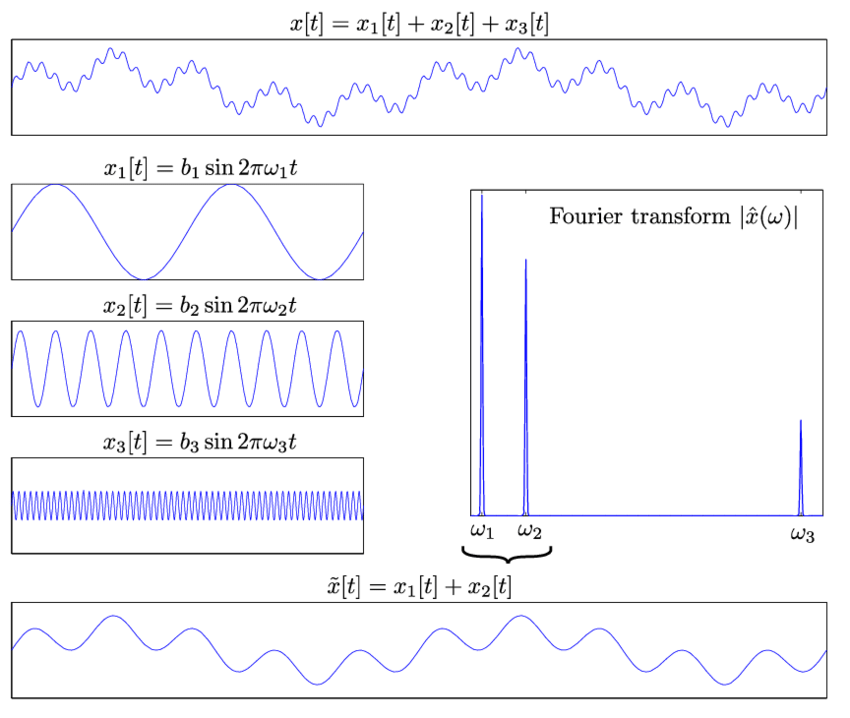
\includegraphics[width=15cm]{imagini/fft.png}
		\caption{Exemplu de transformare al semnalului cu ajutorul Transformatei Rapide Fourier}
		\label{Fig14}
	\end{figure}
	
	\^{I}n Figura \ref{Fig14}, putem observa trei semnale $x_1, x_2, x_3$ care \^{i}mpreun\u{a} formeaz\u{a} semnalul $x$ \c{s}i sunt transformate cu ajutorul Transformatei Rapide Fourier pentru a compune semnalul transformat. 
	
	Analiza Fourier și transformata Fourier dezvăluie că o formă de undă complexă poate fi exprimată ca suma unei serii de unde sinusoidale de amplitudini diferite. Deci un pătrat, triunghi sau orice altă formă de undă care apare în domeniul timpului poate fi reprezentată de mai multe frecvențe individuale diferite de amplitudini variabile în domeniul frecvenței. Aceasta include formele undelor create de instrumentele muzicale, variind de la bătăile ascuțite ale unui tambur până la chitarele electrice cu undă pătrată.
	
	\chapter{Tehnologii utilizate}
		\^{I}n zilele noastre calculatorul este folosit \^{i}n multiple arii \c{s}i are ca scop solu\c{t}ionarea sau optimizarea unor probleme. Acesta poate rezolva diferite sarcini, deoarece este programabil, adic\u{a} a fost realizat pentru a putea solu\c{t}iona orice cerere dat\u{a} de un program.
\bigskip

Un program reprezint\u{a} un set de instruc\c{t}iuni pe care calculatorul le \^{i}ndepline\c{s}te pentru a rezolva o problem\u{a}. Pe l\^{a}ng\u{a} procesul de programare \^{i}n sine, se reg\u{a}sesc \c{s}i alte procese precum testarea, depanarea \c{s}i mentenan\c{t}a codului surs\u{a} care, asigur\u{a} astfel o calitate superioar\u{a} a codului surs\u{a}. Aplica\c{t}ia final\u{a} trebuie s\u{a} \^{i}ndeplineasc\u{a} o serie de propriet\u{a}\c{t}i fundamentale, indiferent de limbajul de programare ales.
\bigskip

O parte din aceste propriet\u{a}\c{t}i sunt:

\begin{enumerate}
	\utb \textit{Fiabilitatea:} proprietate care reprezint\u{a} corectitudinea programului, adic\u{a} \^{i}n ce m\u{a}sur\u{a} aplica\c{t}ia \^{i}ndepline\c{s}te scopul pentru care a fost conceput\u{a}, depinz\^{a}nd de factori externi precum corectitudinea algoritmilor \c{s}i de cuantumul de erori care pot ap\u{a}rea \^{i}n timpul execu\c{t}iei programului. Mai exact, aceasta poate fi v\u{a}zut\u{a} ca o probabilitate.
	
	\utb \textit{Robuste\c{t}ea:} proprietate care define\c{s}te \^{i}n ce m\u{a}sur\u{a} programul soft reacţioneaz\u{a} la evenimente mai pu\c{t}in a\c{s}teptate cum ar fi accesarea datelor indisponibile sau a unei zone de memorie nealocat\u{a}, introducere de date eronate, etc.
	
	\utb \textit{Uzabilitate:} proprietate care vizeaz\u{a} \^{i}n mod direct utilizatorul \c{s}i se refer\u{a} la u\c{s}urin\c{t}a cu care acesta \^{i}şi poate rezolva problemele prin intermediul aplica\c{t}iei dezvoltate.
	
	\utb \textit{Portabilitate:} proprietate care define\c{s}te multitudinea de platforme \c{s}i sisteme de operare pe care poate rula aplica\c{t}ia dezvoltat\u{a}. De asemenea, se refer\u{a} \c{s}i la uşurin\c{t}a cu care se poate muta codul surs\u{a} de pe o platform\u{a} pe alta.
	
	\utb \textit{Mentenabilitate:} proprietate care eviden\c{t}iaz\u{a} u\c{s}urin\c{t}a de a modifica aplica\c{t}ia, anume prin ad\u{a}ugare de noi funcţionalit\u{a}\c{t}i pentru a satisface noi cerin\c{t}e, fixarea problemelor existente sau adaptarea codului la o versiune actual\u{a} aplica\c{t}iei.
	
	\utb \textit{Eficien\c{t}a/Performan\c{t}a:} proprietate care m\u{a}soar\u{a} resursele de timp \c{s}i spa\c{t}iu de memorie folosite la execu\c{t}ia aplica\c{t}iei. Eficien\c{t}a programului const\u{a} \^{i}n minimizarea resurselor utilizate. Un alt aspect important este gestionarea corect\u{a} a memoriei \c{s}i utilizarea unor algoritmi eficien\c{t}i.
\end{enumerate}

\^{I}n continuare urmeaz\u{a} o prezentare detaliat\u{a} privind tehnologiile folosite \^{i}n cadrul acestei lucr\u{a}ri.

\section{Limbajul de programare C{\#}}

	Un limbaj de programare este un limbaj formal care cuprinde un set de instruc\c{t}iuni care produc diferite tipuri de ie\c{s}ire. Limbajele de programare sunt utilizate în programare pentru a implementa algoritmi.
	\bigskip
	
	Majoritatea limbajelor de programare constau \^{i}n instruc\c{t}iuni pentru calculatoare. Exist\u{a} ma\c{s}ini programabile care folosesc un set de instruc\c{t}iuni specifice, mai degrab\u{a} dec\^{a}t limbaje de programare generale.
	\bigskip
	
	Limbajul de programare C{\#} este un limbaj de programare imperativ, obiect-orientat, asem\u{a}n\u{a}tor sintactic cu Java \c{s}i C++. Acesta a fost creat de Microsoft, ini\c{t}ial \^{i}n cadrul proiectului .NET, la sf\^{a}r\c{s}itul anilor 90, fiind un concurent al limbajului Java. Acestea sunt derivate ale limbajului C$++$. Limbajul C{\#} a fost conceput ca s\u{a} fie simplu, modern,	s\u{a} aib\u{a} un scop general \c{s}i s\u{a} fie orientat pe obiecte.
	\bigskip
	
	Acest limbaj con\c{t}ine dou\u{a} categorii de tipuri de date: \textit{tipuri valoare} \c{s}i \textit{tipuri referin\c{t}\u{a}}. Prima categorie con\c{t}ine tipuri simple, precum: char, int, float, dar \c{s}i tipurile enumerare \c{s}i structur\u{a}, fiind alocate pe stiv\u{a} sau inline \^{i}ntr-o structur\u{a}. Cea de-a doua categorie con\c{t}ine tipurile interfa\c{t}\u{a}, delegat \c{s}i tablou. Un aspect important al limbajului de programare C{\#} este faptul c\u{a} toate tipurile de date sunt derivate direct sau indirect din tipul de date System.Object\cite{limbaj}.
	\bigskip
	
	Astfel, se pot crea aplica\c{t}ii web prin intermediul ASP.NET, aplica\c{t}ii desktop prin WPF(Windows Presentation Foundation) sau aplica\c{t}ii mobile pe Windows Phone. Common Language Runtime(CLR) gestioneaz\u{a} execu\c{t}ia programelor .NET, fiind un Virtual Machine(VM) care ruleaz\u{a} Intermediate Language(IL) \c{s}i ofer\u{a} multiple servicii, precum gestionarea memoriei, securitate, gestionare de excep\c{t}ii, garbage collector, dar \c{s}i altele. 
	\bigskip
	
	\^{I}n cadrul acestui studiu, limbajul de programare a fost folosit pentru a realiza implementarea modelului acustic, iar rezultatele acestuia au fost ilustrate cu ajutorul platformei Unity, dar \c{s}i cu ajutorul limbajului de programare Python.
	
\section{Limbajul de programare Python \c{s}i biblioteca matplotlib}

	Python este un limbaj de programare interpretat, obiect orientat, de nivel înalt, cu semantică dinamică. Structurile sale de date încorporate la nivel înalt, combinate cu tastarea dinamică și legarea dinamică, îl fac foarte atractiv pentru dezvoltarea rapidă a aplicațiilor, precum și pentru a fi utilizat ca limbaj de scriptare sau lipici pentru a conecta componentele existente împreună. Sintaxa simplă, ușor de învățat accentuează lizibilitatea și, prin urmare, reduce costul întreținerii programului. Python acceptă module și pachete, ceea ce încurajează modularitatea programului și reutilizarea codului.
	\bigskip
	
	Acest studiu folose\c{s}te biblioteca matplotlib pentru a reprezenta rezultate comparative pentru func\c{t}ia de r\u{a}spuns \^{i}n timp sau sunetul dup\u{a} convolu\c{t}ie pe mai multe microfoane. Aceasta este o bibliotecă ultil\u{a} pentru crearea de vizualizări statice, animate și interactive în Python. Matplotlib poate fi utilizat în scripturi Python, shell-urile Python și IPython, servere de aplicații web și diverse seturi de instrumente grafice de interfață cu utilizatorul\cite{python}.
	
\section{Platforma Unity}

	O platform\u{a}(IDE- Integrated Development Environment) este o aplica\c{t}ie software care ofer\u{a} facilit\u{a}\c{t}i programatorilor pentru dezvoltarea de soft. O platform\u{a} este alc\u{a}tuit\u{a} din cel pu\c{t}in un editor de cod surs\u{a}, instrumente de automatizare a construc\c{t}iilor \c{s}i un depanator.
	\bigskip
	
	Un singur program \^{i}n care se realizeaz\u{a} dezvoltarea unui soft reprezint\u{a} o platform\u{a}(IDE). Aceast\u{a} platform\u{a} ofer\u{a} multe caracteristici pentru autorizare, modificare, compilare, implementare \c{s}i depanare a produsului soft. Unele platforme sunt specializate pe un limbaj de programare specific, oferind un set de caracteristici care se potrivesc cu paradigma de programare a acelui limbaj. Cu toate acestea, exist\u{a} multe IDE-uri  care suport\u{a} mai multe limbaje de programare.
	\bigskip
	
	Platforma Unity este folosit\u{a} \^{i}n general pentru a crea jocuri \c{s}i poate rula pe mai multe platforme. A fost dezvoltat de Unity Technologies \c{s}i lansat \^{i}n 2005 la Apple Inc's Worldwide Developers Conference ca fiind un game engine exclusiv pentru macOS. 
	\bigskip
	
	Unity este principala platform\u{a} mondial\u{a} pentru crearea \c{s}i operarea de con\c{t}inut 3D interactiv, \^{i}n timp real, oferind instrumente pentru a crea jocuri \c{s}i pentru a le publica pe o gam\u{a} larg\u{a} de dispozitive. Platforma de baz\u{a} Unity permite echipelor creative s\u{a} fie mai productive \^{i}mpreun\u{a}.
	\bigskip
	
	De-a lungul anilor, aceast\u{a} platform\u{a} s-a dezvoltat reu\c{s}ind ast\u{a}zi s\u{a} sus\c{t}in\u{a} peste 25 de platforme. Platforma poate fi utilizat\u{a} pentru a crea jocuri 2D \c{s}i 3D, realitate virtual\u{a} \c{s}i realitate augmentat\u{a}. Unity este utilizat nu numai pentru jocuri video, c\^{a}t \c{s}i \^{i}n domeniul filmelor, arhitecturii, ingineriei si construc\c{t}iilor\cite{unity}.
	
\section{Platforma Blender}
	
	Blender este o aplica\c{t}ie software de grafic\u{a} 3D folosit\u{a} pentru crearea de informa\c{t}ii, efecte vizuale, art\u{a}, modele de tip\u{a}rire 3D, grafic\u{a} de mi\c{s}care, aplica\c{t}ii 3D interactive \c{s}i jocuri pe calculator. Aceasta este cross-platform \c{s}i permite map\u{a}ri UV, folosirea materialelor, a shaderelor, a mesh-urilor f\u{a}r\u{a} probleme.
	\bigskip
	
	\^{I}n acest studiu, programul a fost folosit pentru a putea realiza \^{i}nc\u{a}perea sferic\u{a} din aplica\c{t}ie, \^{i}ntruc\^{a}t era nevoie de un soft ce trebuia s\u{a} permit\u{a} crearea unei fi\c{s}ier de tipul ,,obj'' care s\u{a} con\c{t}in\u{a} o sfer\u{a} cu normalele inversate pentru a putea plasa alte elemente \^{i}n\u{a}untrul acesteia.
	
\section{Biblioteca NWaves, XCharts \c{s}i StandaloneFileBrowser}

	Biblioteca NWaves a fost ini\c{t}ial destinat\u{a} cercet\u{a}rii, vizualiz\u{a}rii \c{s}i pred\u{a}rii elementelor de baz\u{a} ale program\u{a}rii DSP(Digital Signal Processing) \c{s}i a sunetului. To\c{t}i algoritmii sunt implementa\c{t}i \^{i}n limbajul de programare C{\#}, c\^{a}t mai simplu posibil \c{s}i au fost proiecta\c{t}i \^{i}n principal pentru procesarea offline(\^{i}n prezent exist\u{a} \c{s}i multe metode online)\cite{nwaves}.
	\bigskip
	
	Aceast\u{a} bibliotec\u{a} este una open source destinat\u{a} proces\u{a}rii digitale a semnalelor audio, \^{i}nglob\^{a}nd multiple func\c{t}ionalit\u{a}\c{t}i pentru acest domeniu. \^{I}n cadrul studiului, biblioteca a fost folosit\u{a} pentru citirea/creearea fi\c{s}ierelor cu extensia \textit{,,wav"}, dar \c{s}i pentru convolu\c{t}ia sunetelor.
	\bigskip

	XCharts este o bibliotec\u{a} puternic\u{a}, u\c{s}or de utilizat \c{s}i de configurat pentru vizualizarea datelor \^{i}n contextul platformei Unity. Acest proiect a fost dezvoltat sub Unity 2017 \c{s}i .NET 3.5\cite{xcharts}.
	\bigskip
	
	Diferite componente \c{s}i date pot fi  combinate \^{i}n diferite tipuri de diagrame. O component\u{a} XCharts este \^{i}mp\u{a}r\c{t}it\u{a} \^{i}ntr-o component\u{a} principal\u{a} \c{s}i \^{i}n una sau mai multe componente secundare, unde cea principal\u{a} con\c{t}ine toate componentele secundare. 
	\bigskip
	
	Biblioteca a fost folosit\u{a} \^{i}n contextul acestei lucr\u{a}ri pentru a ilustra date statistice privind sunetul, precum: func\c{t}ia de r\u{a}spuns la impuls \^{i}n frecven\c{t}\u{a} \c{s}i \^{i}n timp, magnitudinea, faza, timpul, dar \c{s}i altele.
	\bigskip

	Biblioteca StandaloneFileBrowser este una cross-platform ce permite lucrul cu fi\c{s}iere pentru platforma Unity\cite{standalone}. Aceasta a fost folosit\u{a} \^{i}n realizarea aplica\c{t}iei pentru a permite deschiderea \c{s}i utilizarea fi\c{s}ierelor \textit{,,wav"} pentru a putea crea input-ul pentru modelul acustic.
	

	
	\chapter{Etapele elementare pentru implementarea aplica\c{t}iei}
		Acest capitol va descrie detaliat algoritmul de modelare acustic\u{a} \^{i}n spa\c{t}ii interioare folosind metoda Ray-Tracing \c{s}i va con\c{t}ine etapele elementare pentru implementarea acestuia. \c{T}in\^{a}nd cont de toate acestea, aplica\c{t}ia poate fi \^{i}mp\u{a}r\c{t}it\u{a} \^{i}n patru etape:
\begin{enumerate}
	\utb Calcul geometric
	\begin{itemize}
		\item Sfera lui Fibonacci - este un algoritm ce presupune distribuirea punctelor în mod uniform pe suprafața unei sfere
		\item Propagarea razelor - presupune distribuirea unui număr finit de raze în încăpere pornind de la niște puncte de start și ținând cont de numărul maxim de reflexii pe care îl poate avea o rază și de distanța maximă a acesteia
		\item Selec\c{t}ia razelor - dintr-un număr cunoscut de raze se vor selecta doar acelea care îndeplinesc anumite condiții
	\end{itemize}
	\utb Calcul fizic
	\begin{itemize}
		\item Calculul intensit\u{a}\c{t}ilor - pentru fiecare punct de coliziune al unei raze trebuie calculată intensitatea ținând cont de suprafețele de impact
		\item Calculul presiunilor - fiecare intensitate calculată la pasul anterior trebuie transformată în presiune ținând cont de temperatura din mediu, viteza sunetului prin aer și de densitatea aerului
		\item Func\c{t}ia de r\u{a}spuns la frecven\c{t}\u{a} \c{s}i func\c{t}ia de r\u{a}spuns la impuls - este necesar să cunoaștem valorile acestor funcții pentru a putea obține rezultatele finale
		\item Calculul distan\c{t}elor - pentru fiecare rază trebuie să cunoaștem lungimea acesteia
		\item Calculul timpilor - pentru fiecare rază trebuie să cunoaștem momentul la care aceasta a lovit un anumit obiect, în cazul acestui studiu obiectul de interes este microfonul
	\end{itemize}
	\utb Post-procesare 
	\begin{itemize}
		\item Convolu\c{t}ia sunetului - presupune preluarea funcției de răspuns la impuls și a sunetului care a fost difuzat în încăpere si combinarea acestora pentru a obține soluția
	\end{itemize}
	\utb GUI (Graphical User Interface)
\end{enumerate}
 

Astfel, pentru a realiza acest model trebuie s\u{a} \^{i}ncepem prin a distribui uniform razele plec\^{a}nd de la surs\u{a}, dup\u{a} care trebuie s\u{a} select\u{a}m razele care intersecteaz\u{a} microfoanele din \^{i}nc\u{a}pere. Pentru a ob\c{t}ine performan\c{t}\u{a} este necesar s\u{a} excludem acele raze care nu ajung pe nici unul dintre microfoane sau acele raze care intersecteaz\u{a} microfoanele, dar sunt foarte asem\u{a}n\u{a}toare \c{s}i s\u{a} pastr\u{a}m doar una dintre aceste raze asemănătoare pentru a reduce din costul computațional.

 
Pentru pasul urm\u{a}tor calcul\u{a}m intensit\u{a}\c{t}ile pentru fiecare raz\u{a} pe care mai apoi le transform\u{a}m \^{i}n presiuni. Urm\u{a}toarea etap\u{a} presupune calculul frecven\c{t}elor \c{s}i calcularea fazelor. Dup\u{a} ce ace\c{s}ti pa\c{s}i au fost realizați, mai este nevoie doar s\u{a} calcul\u{a}m distan\c{t}ele \c{s}i timpii pentru ca mai departe s\u{a} ob\c{t}inem func\c{t}ia de r\u{a}spuns la impuls \c{s}i func\c{t}ia de r\u{a}spuns în frecven\c{t}\u{a}.

  
Acum c\u{a} am considerat toate aceste etape mai rămâne doar s\u{a} putem interpreta rezultatul algoritmului nostru. Astfel, cu ajutorul convolu\c{t}iei ajungem s\u{a} ascult\u{a}m solu\c{t}ia algoritmului, iar modelul nostru acustic este complet.

\section{Ghid de utilizare al aplica\c{t}iei}

	Acustica face parte din domeniul fizicii \c{s}i se ocup\u{a} cu studiul undelor mecanice \^{i}n gaze, lichide, solide \c{s}i este prezent \^{i}n toate aspectele societ\u{a}\c{t}ii actuale, \^{i}ns\u{a} predominant \^{i}n domeniul industriei pentru controlul zgomotului. Aceast\u{a} ramur\u{a} implic\u{a} \c{s}i studiul sunetelor, vibra\c{t}iilor, ultrasunetelor \c{s}i infrasunetelor. Un model acustic va implica, \^{i}n cel mai generic mod, simularea c\u{a}ilor pe care sunetul le parcurge de la surs\u{a} la destina\c{t}ie. Cel mai adesea, aceste modele presupun rezolvarea integralei Helmoltz-Kirchoff \cite{helmoltz} folosind diverse abord\u{a}ri de calcul, precum: solu\c{t}ii numerice ale ecua\c{t}iei de und\u{a}, aproxim\u{a}ri de \^{i}nalt\u{a} frecven\c{t}\u{a} ale ecua\c{t}iei de und\u{a}, dar \c{s}i modele statistice. Modelul pe care \^{i}l propune acest studiu face parte din cea de-a doua categorie. Modelul acustic va con\c{t}ine etapa de calcul geometric, etapa de calcul fizic, convolu\c{t}ia sunetului \c{s}i realizarea unei interfe\c{t}e ce permite validarea acestor rezultate.
	 
	
	\c{T}in\^{a}nd cont de toate aceste elemente este foarte important s\u{a} re\c{t}inem c\u{a} aceste etape se afl\u{a} \^{i}ntr-o leg\u{a}tur\u{a} str\^{a}ns\u{a} \c{s}i se bazeaz\u{a} unele pe celelalte. Astfel, ne putem da seama c\u{a} calculul geometric este o etap\u{a} deosebit de important\u{a}, \^{i}ntruc\^{a}t modul \^{i}n care distribuim razele \^{i}n \^{i}nc\u{a}pere \c{s}i selec\c{t}ia acestora dicteaz\u{a} performan\c{t}a modelului \c{s}i optimalitatea acestuia. Algoritmii de post-procesare sunt folosi\c{t}i, de obicei, pentru a suprima zgomotul sau orice artefact creat \^{i}n cadrul primelor dou\u{a} etape, adic\u{a} calculul geometric \c{s}i cel fizic, concentr\^{a}ndu-se pe eliminarea distorsiunii \c{s}i a ecoului.
	
	Aplicația dezvoltată în această lucrare cuprinde toate etapele enunțate mai sus și urmează a fi detaliate în paginile ce urmează. Pentru început va fi prezentat modul în care arată aplicația și funcționalitățile acesteia, urmând să fie prezentat și modul în care a fost creat modelul acustic.
	
	Interfa\c{t}a aplica\c{t}iei a fost realizat\u{a} cu ajutorul platformei Unity. \^{I}nc\u{a}perile dreptunghiulare au fost construite folosind formele 3D puse la dispozi\c{t}ie de c\u{a}tre aceast\u{a} platform\u{a}, iar \^{i}nc\u{a}perea sferic\u{a} a fost creat\u{a} \^{i}n Blender. Pentru cea din urm\u{a} camer\u{a} a fost folosit un obiect de tip sfer\u{a} pentru care au fost inversate normalele. Fiecare spa\c{t}iu folose\c{s}te culori \c{s}i materiale potrivite utiliz\^{a}nd Unity Material, o clas\u{a} care permite utilizatorului s\u{a} animeze un obiect prin intermediul propriet\u{a}\c{t}ilor de care dispune aceast\u{a} clas\u{a}.
	
	Pentru acest studiu au fost g\^{a}ndite trei \^{i}nc\u{a}peri: dou\u{a} dreptunghiulare \c{s}i una sferic\u{a}. Prima \^{i}nc\u{a}pere dreptunghiular\u{a} are dimenisunea de 4x5m, iar cea de-a doua are 30x30m. \^{i}nc\u{a}perea sferic\u{a} are raza 5m. Acestea pot fi vizualizate \^{i}n Figura \ref{rooms}. Pentru \^{i}nc\u{a}perile dreptunghiulare sursa a fost pozi\c{t}ionat\u{a} \^{i}n centru, iar pentru \^{i}nc\u{a}perea sferic\u{a} sursa a fost pozitionat\u{a} astfel \^{i}nc\^{a}t s\u{a} apar\c{t}in\u{a} unui cerc pe care vor fi plasate microfoanele. Formele încăperilor au fost alese pentru a reprezenta o parte din formele de bază pe care o încăpere le poate avea.
	
	\begin{figure}[!htb]%
		\begin{subfigure}[b]{.3\textwidth}
			\centering
			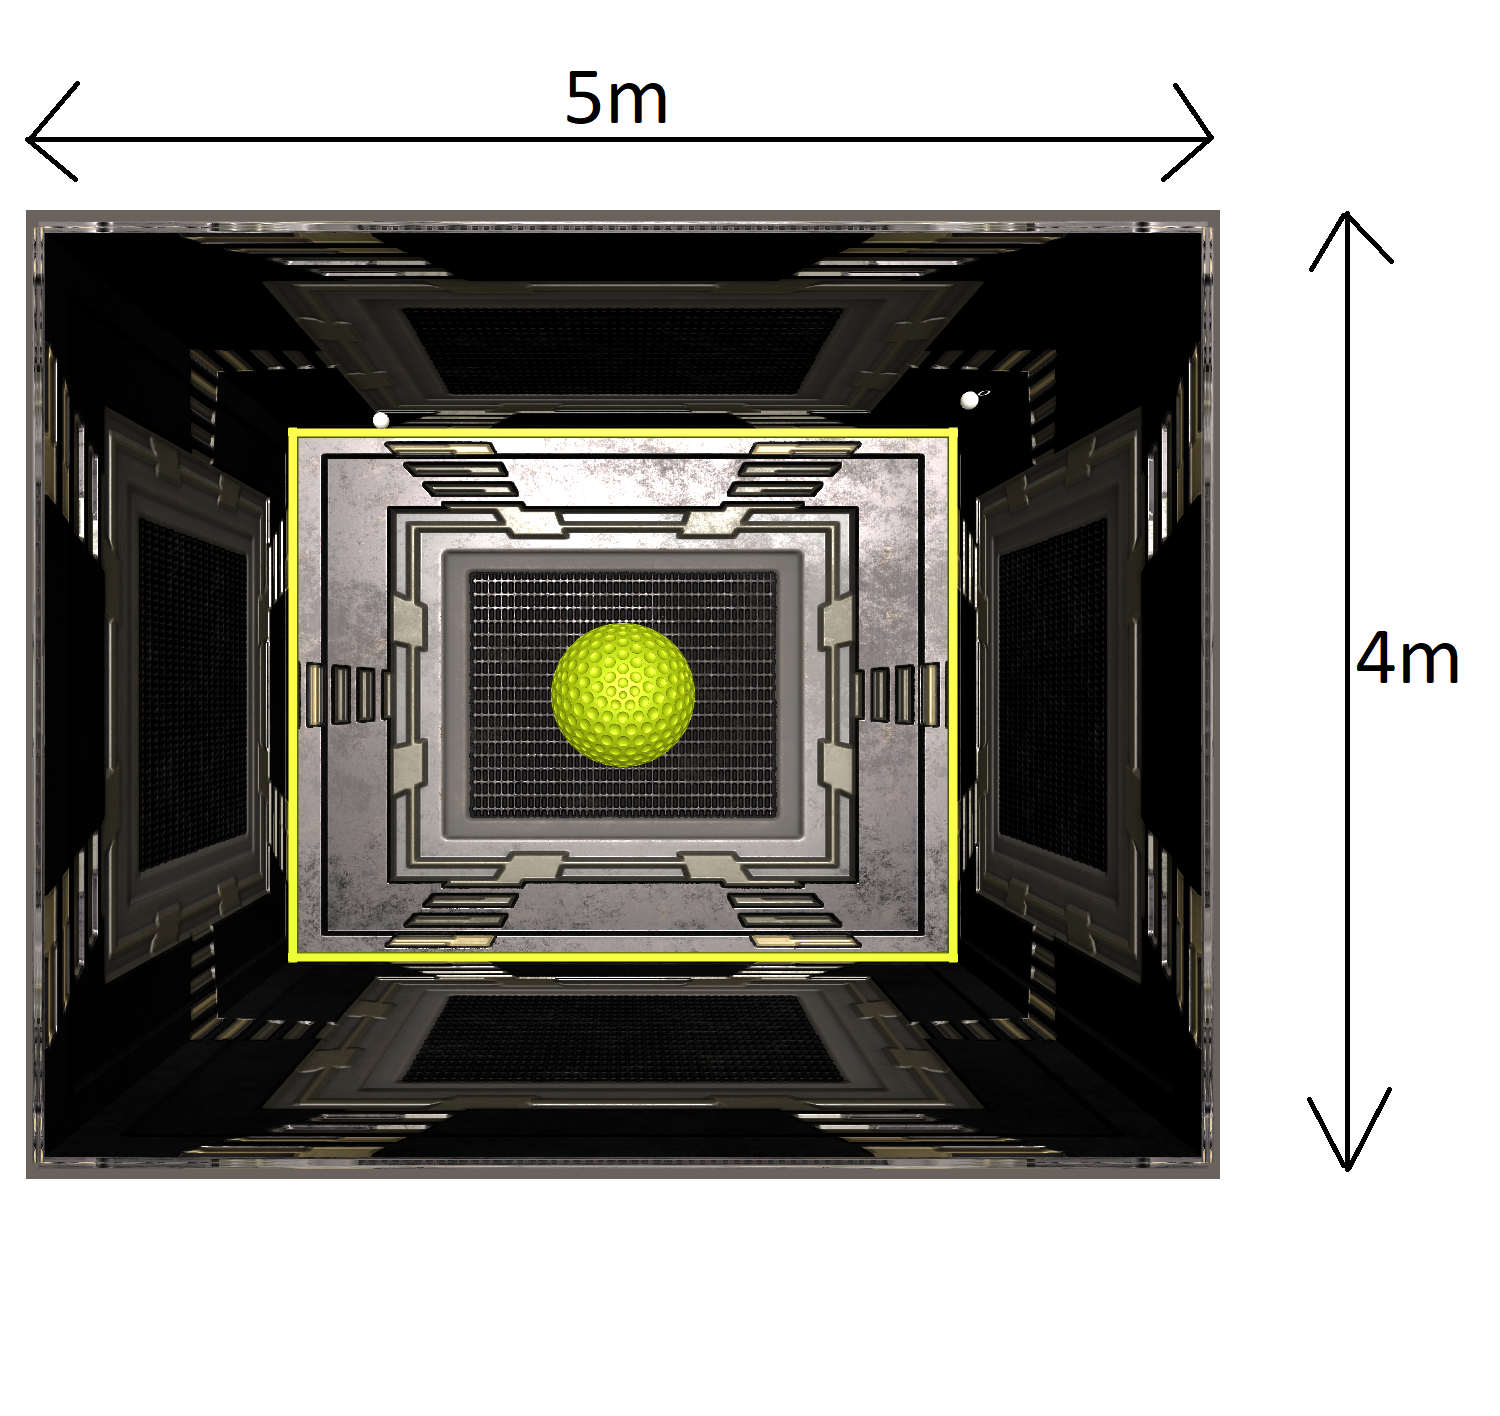
\includegraphics[width=1\linewidth]{imagini/smallRoom.png} 
			\caption{\^{I}nc\u{a}perea dreptunghiular\u{a} mic\u{a}}
			%\label{fig:sub-fig}
		\end{subfigure}
		\hfill
		\begin{subfigure}[b]{.3\textwidth}
			\centering
			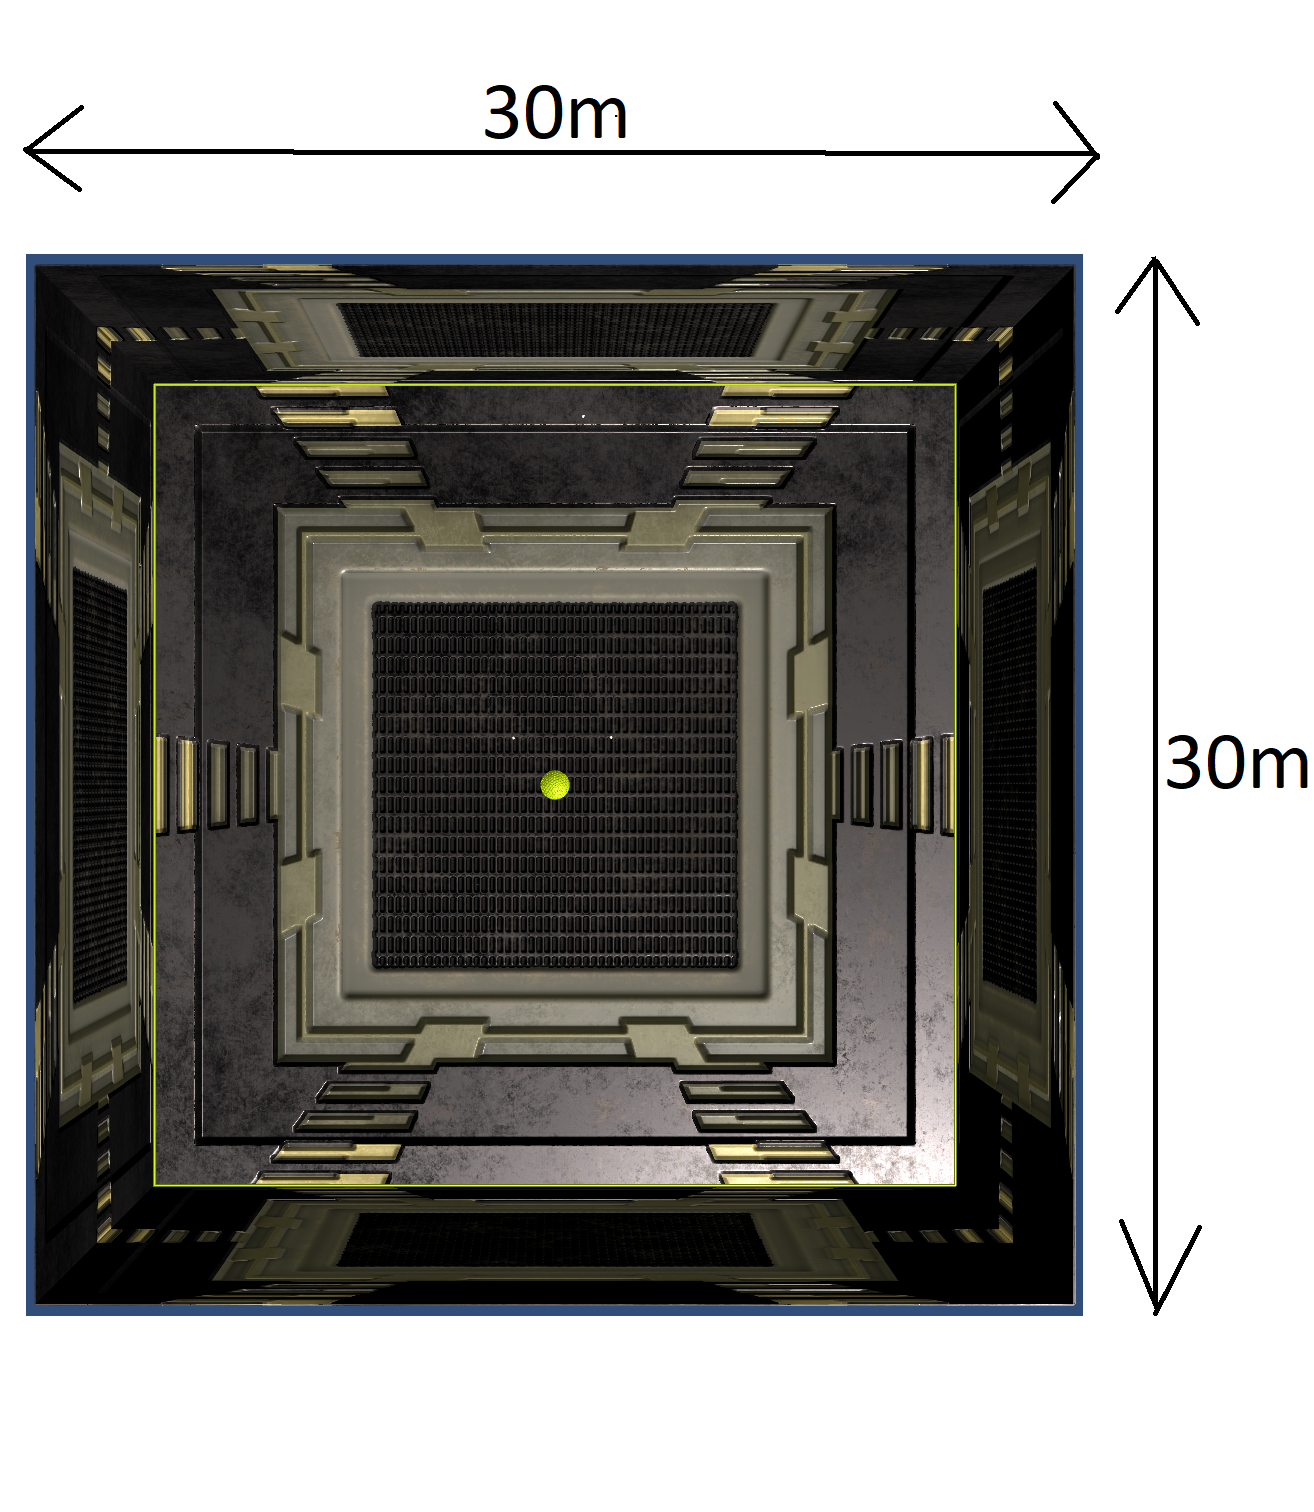
\includegraphics[width=1\linewidth]{imagini/bigRoom.png}
			\caption{\^{I}nc\u{a}perea dreptunghiular\u{a} mare}
			%\label{fig:sub-second}
		\end{subfigure}
		\hfill
		\begin{subfigure}[b]{.3\textwidth}
			\centering
			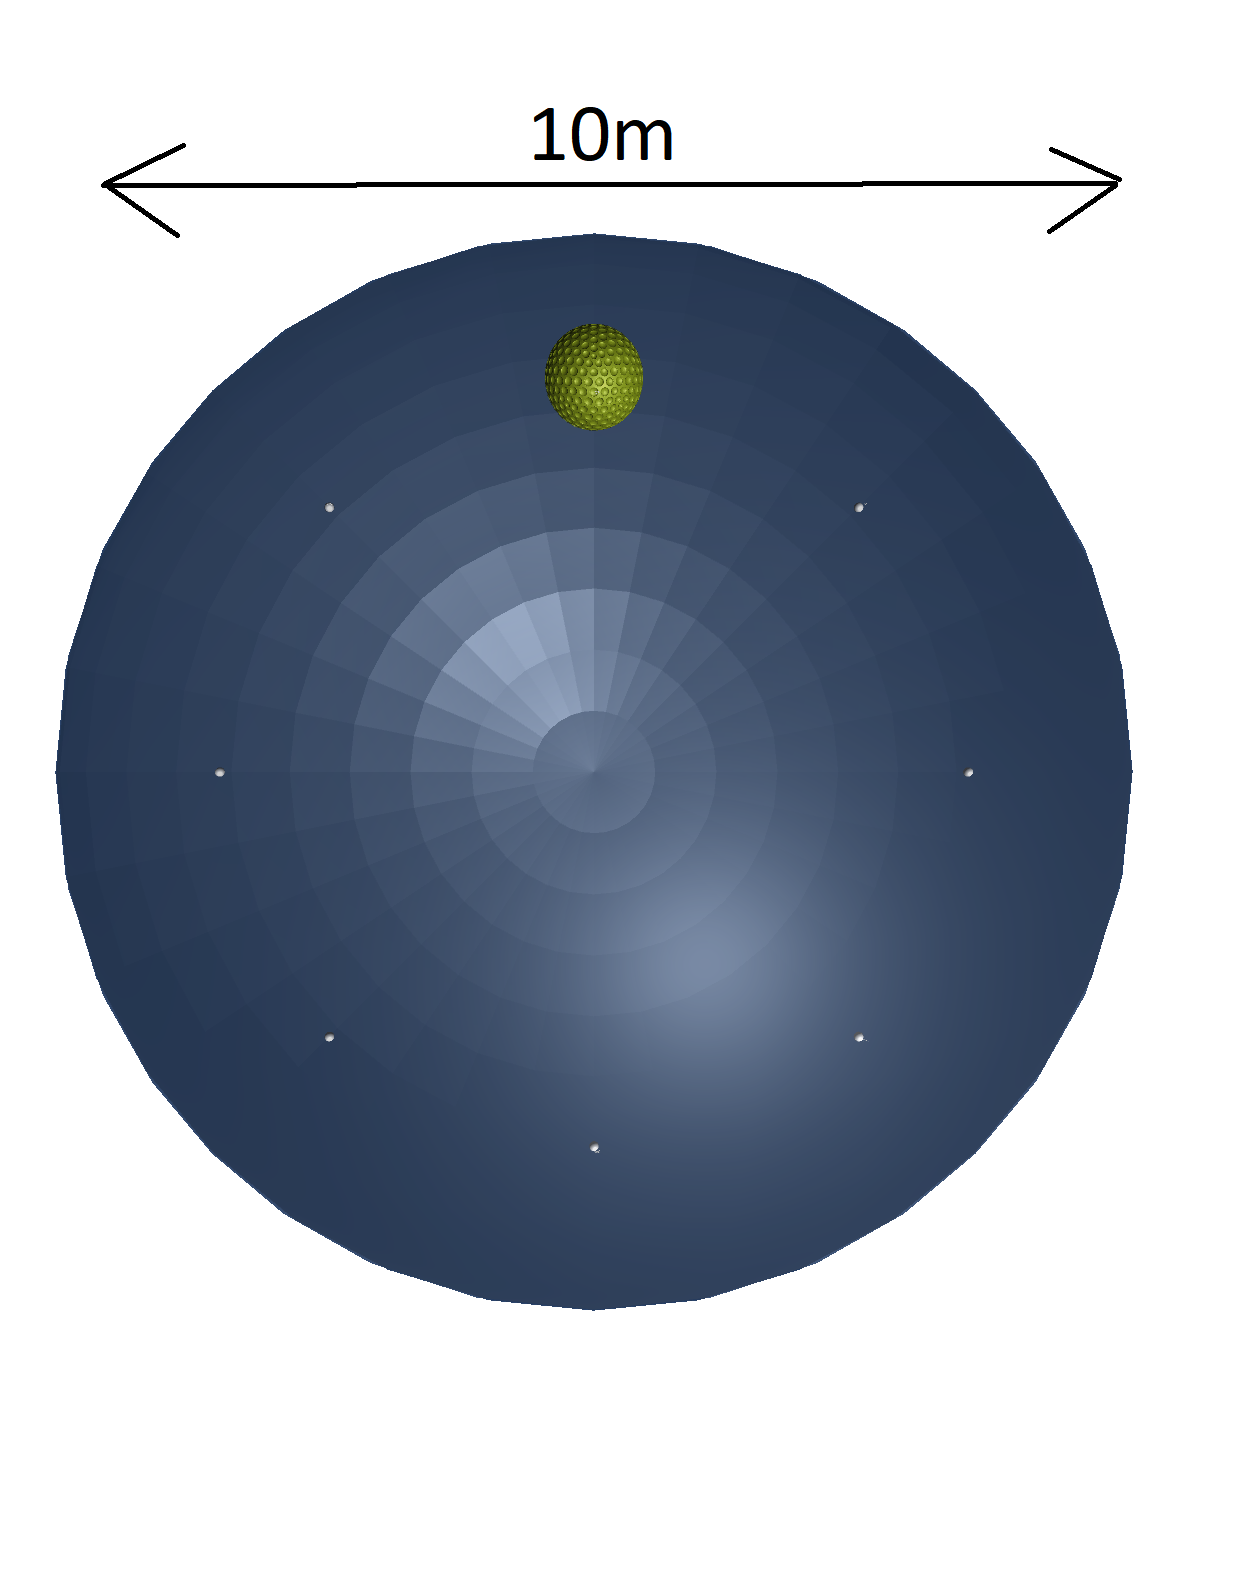
\includegraphics[width=1\linewidth]{imagini/sphericRoom.png}
			\caption{\^{I}nc\u{a}perea sferic\u{a}}
			%\label{fig:sub-third}
		\end{subfigure}
		
		\caption{Tipuri de încăperi studiate}
		\label{rooms}
	\end{figure}
	
	 
	Meniurile aplica\c{t}iei au fost realizate tot cu ajutorul platformei Unity folosind elemente de UI precum: Canvas, Panel, Button, Dropdown, Label, Input, Text, dar \c{s}i altele. Canvas-ul este un element ce con\c{t}ine o arie \^{i}n interiorul c\u{a}reia ar trebui s\u{a} se afle toate celelalte elemente de UI, iar un Panel este utilizat pentru a sus\c{t}ine mai multe elemente precum Button, Label, Input, Dropdown, Text etc. De asemenea, pentru butoane au fost alese imagini intuitive care s\u{a} u\c{s}ureze folosirea acestora, dar \c{s}i un font adecvat pentru text astfel \^{i}nc\^{a}t s\u{a} fie lizibil pentru utilizator.
	
	Aplicația conține un meniu principal care permite selecția camerei pe care dorim să o alegem, dar și un buton de exit. După ce intrăm în una dintre încăperi vom avea posibilitatea să ne plimbăm prin cameră sau să alegem una dintre cele 3 opțiuni: deschiderea meniului ce setează datele de intrare pentru modelul acustic, rularea acestuia și observarea rezultatelor; deschiderea meniului pentru vizualizarea tuturor razelor sau vizualizarea unei singure raze; butonul de back care permite alegerea unei alte camere.
	
	\begin{figure}[!htb]
		\centering
		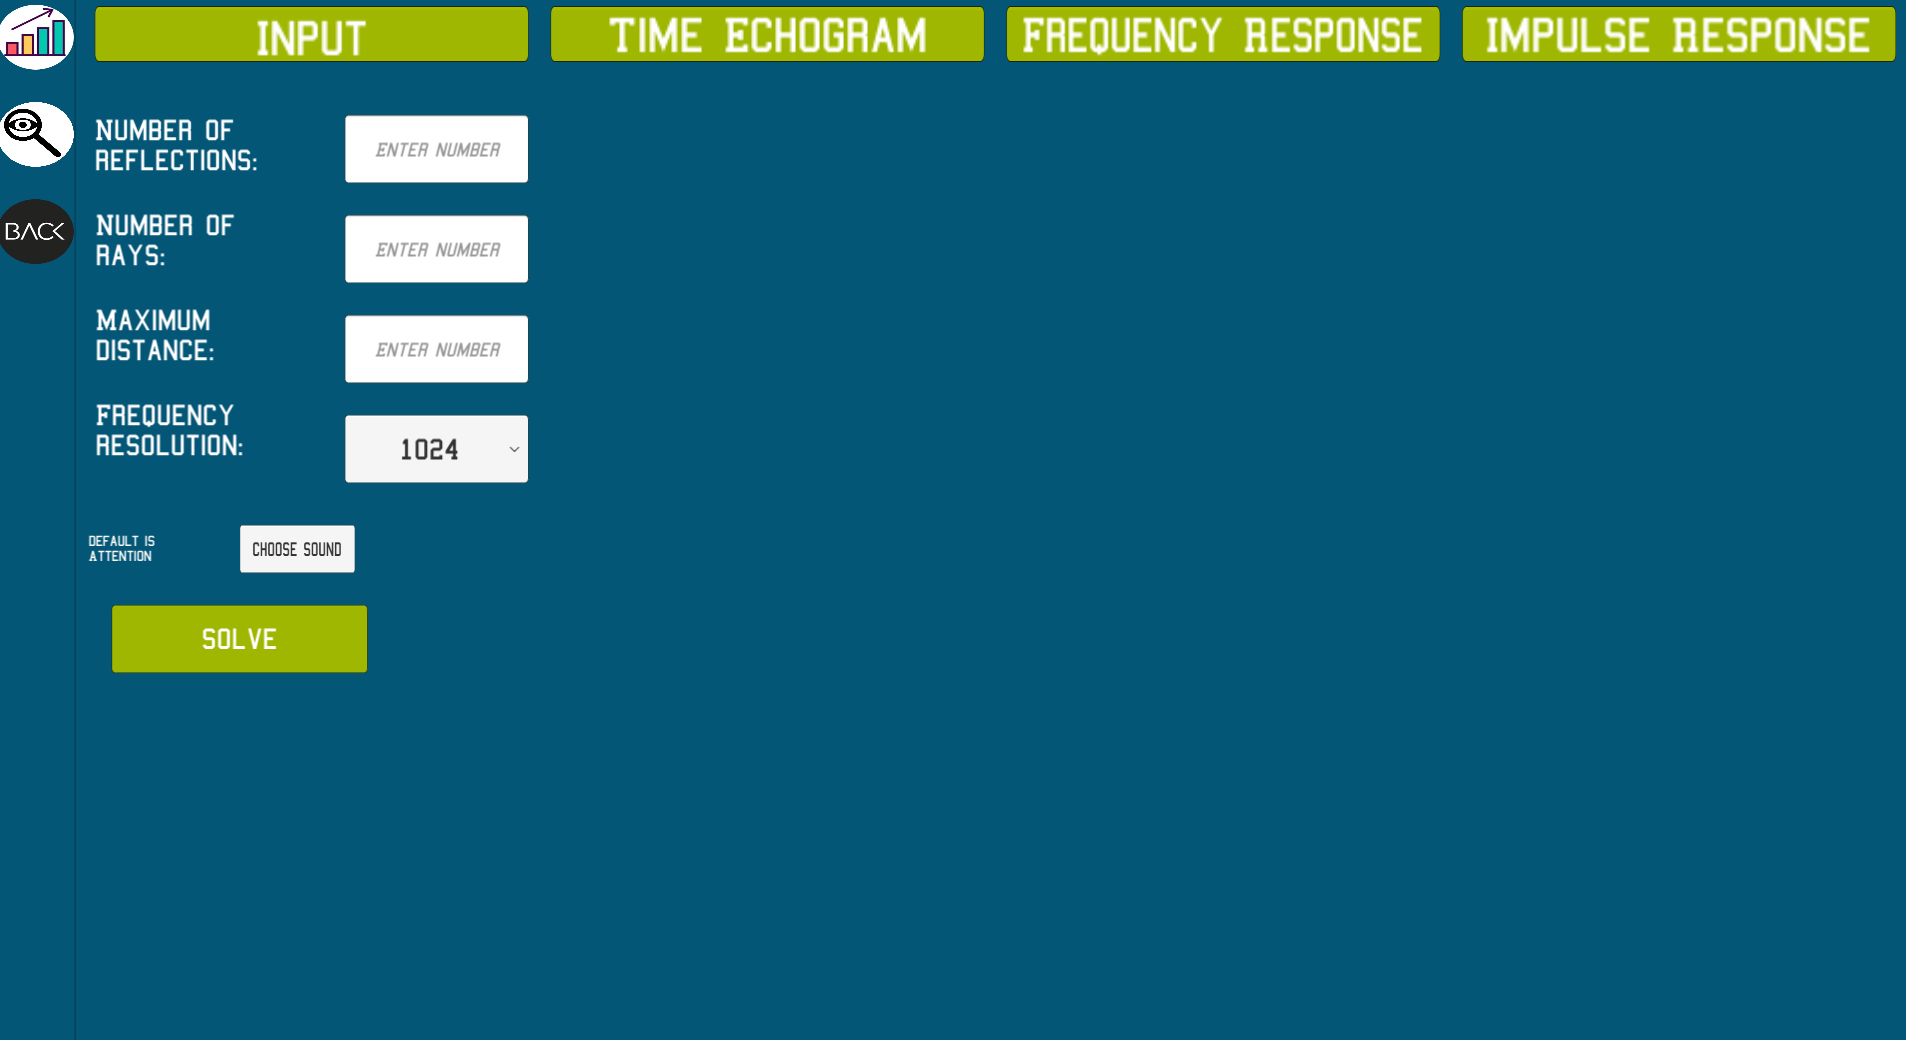
\includegraphics[width=1\linewidth]{imagini/input.png}
		\caption{Meniul pentru setarea configura\c{t}iei}
		\label{inputFig}
	\end{figure}

	\^{I}n Figura \ref{inputFig} putem observa meniul care ne ajut\u{a} s\u{a} set\u{a}m valorile pentru care dorim s\u{a} analizăm ce se \^{i}nt\^{a}mpl\u{a} \^{i}ntr-o \^{i}nc\u{a}pere cu sunetul. Cu ajutoul acestei ferestre avem posibilitatea de a parametriza algoritmul \c{s}i putem stabili care este num\u{a}rul maxim de reflexii permis pentru o raz\u{a}, num\u{a}rul de raze ce se vor \^{i}mpr\u{a}\c{s}tia \^{i}n camer\u{a}, distan\c{t}a maxim\u{a} permis\u{a} pentru o raz\u{a}, pasul de frecvență \c{s}i sunetul ce va fi difuzat \^{i}n \^{i}nc\u{a}pere. De asemenea, flexibiltatea aplicației este sporită prin includerea celor 3 ferestre: \textit{TIME ECHOGRAM, FREQUENCY RESPONSE} \c{s}i \textit{IMPULSE RESPONSE}, oferind o gamă variată de a vizualiza \c{s}i interpreta rezultatele.
	 
	
	\begin{figure}[!htb]
		\centering
		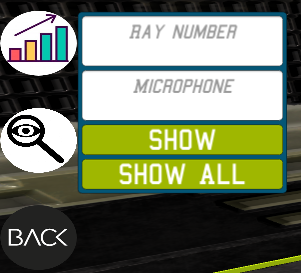
\includegraphics[width=6cm]{imagini/rayMenu.png}
		\caption{Meniul pentru vizualizarea razelor}
		\label{rayMenu}
	\end{figure}

	Aplica\c{t}ia permite at\^{a}t vizualizarea tuturor razelor din \^{i}nc\u{a}pere folosind butonul ,,Show all'', c\^{a}t \c{s}i vizualizarea unei raze individual prin intermediul butonului ,,Show'', aceste lucruri fiind ilustrare \^{i}n Figura \ref{rayMenu}.
	
	Pentru a putea observa razele din încăpere sau chiar pentru a putea să analizăm camera în sine, am implementat două moduri pentru a vizualiza camera. Un mod permite mutarea prin încăpere folosind WASD și mouse-ul pentru a schimba direcția utilizatorului și un mod care permite vizualizarea de sus a încăperii și mutarea utilizatorului trăgând cu mouse-ul într-o anumită direcție. Aceste două opțiuni pot fi utilizate folosind tastele ,,O'' și ,,P'' de pe tastatură, aplicația este setată să utilizeze implicit primul mod de vizualizare.
	 
	Mai mult de at\^{a}t, pentru a realiza graficele ce definesc o parte din rezultatele solver-ului a fost folosit\u{a} biblioteca XCharts. Aceasta a fost utilizată \^{i}n aplica\c{t}ie pentru a crea un mod de a vizualiza func\c{t}ia de r\u{a}spuns la impuls, func\c{t}ia de r\u{a}spuns \^{i}n frecven\c{t}\u{a}, dar \c{s}i ecograma de timp.
	
	
	Biblioteca StandaloneFileBrowser a fost folosit\u{a} \^{i}n interfa\c{t}a aplica\c{t}iei pentru a permite utilizatorului s\u{a} \^{i}ncarce un fi\c{s}ier cu extensia ,,.wav'' pentru a putea fi folosit mai departe drept parametru pentru modelul acustic \^{i}ntr-un mod c\^{a}t mai intuitiv.


\section{Calcul geometric}

	Calculul geometric presupune simularea geometriei unei \^{i}nc\u{a}peri. Pentru acest lucru vom considera ca date de intrare suprafe\c{t}ele \^{i}nc\u{a}perii, sursa audio \c{s}i microfoanele plasate \^{i}n \^{i}nc\u{a}pere. Cu ajutorul acestora vom putea distribui uniform raze \^{i}n \^{i}nc\u{a}pere folosind algoritmul sferei lui Fibonacci \c{s}i vom p\u{a}stra doar acele raze de care avem nevoie cu ajutorul unui algoritm pentru reducerea razelor duplicat. Aceste subetape urmeaz\u{a} a fi prezentate \^{i}n urm\u{a}toarele pagini.
	
\subsection{Sfera lui Fibonacci}

	De-a lungul timpului, \^{i}n literatura matematic\u{a}, au existat multiple \^{i}ncerc\u{a}ri pentru solu\c{t}ionarea problemei distribuirii uniforme a punctelor pe o sfer\u{a}. Din p\u{a}cate, cu excep\c{t}ia c\^{a}torva cazuri speciale, nu este posibil s\u{a} se distribuie \^{i}n mod egal punctele pe suprafa\c{t}a unei sfere.
	 

	Astfel, vom prezenta modul \^{i}n care vor fi distribuite razele pe sursa audio \^{i}n contextul algoritmului nostru. Sursa va fi reprezentat\u{a}, \^{i}n modelul propus, de o sfer\u{a} pe care se vor alege puncte uniform distribuite din care vor porni razele.
	 
	
	Chiar dac\u{a} seturile de puncte Fibonacci nu reprezint\u{a} cea mai bun\u{a} distribu\c{t}ie global\u{a} a punctelor pe o sfer\u{a}, ele ofer\u{a} propriet\u{a}\c{t}i excelente de e\c{s}antionare \c{s}i sunt extrem de simple de construit fa\c{t}\u{a} de alte modele.
	 
	
	Una dintre cele mai mari provoc\u{a}ri pentru acest algoritm este determinat de faptul c\u{a} distribu\c{t}ia optim\u{a} depinde \^{i}n mod critic de func\c{t}ia obiectiv pe care o utiliz\u{a}m, \^{i}n cazul nostru este dependent\u{a} de $N$, num\u{a}rul de puncte pe care vrem s\u{a} \^{i}l distribuim pe sfer\u{a}.
	 
	
	\^{I}n Figura \ref{Fig13}, se poate observa impactul pe care $N$ \^{i}l are \^{i}n cadrul algoritmului. Cu c\^{a}t $N$ este mai mare, cu at\^{a}t punctele pe sfer\u{a} sunt mai bine distribuite.
	 
	
	\begin{figure}[!htb]
		\centering
		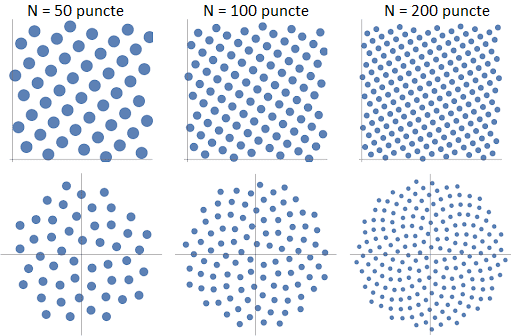
\includegraphics[width=0.92\linewidth]{imagini/fibo.png}
		\caption{Rezultate pentru algoritmul sferei lui Fibonacci \cite{fibo}}
		\label{Fig13}
	\end{figure}
	
	Acest algoritm se bazeaz\u{a} pe o deplasare \^{i}n spiral\u{a} pe suprafa\c{t}a sferei incremental cu unghiul de aur, care este legat de raportul de aur. Dou\u{a} cantit\u{a}\c{t}i, a \c{s}i b, se afl\u{a} \^{i}n raportul de aur dac\u{a}: $\dfrac{a}{b} = \dfrac{a+b}{a} = \varphi$, unde $a>b$, iar acest raport este aproximativ egal cu $\varphi = \dfrac{1+\sqrt{5}}{2}$. Unghiul de aur, $\vartheta$, este definit \^{i}n func\c{t}ie de raportul de aur astfel: $\vartheta = 2\pi(2- \varphi)$. 
	 
	
	\begin{algorithm}
		\caption{Sfera lui Fibonacci}
		\label{fiboLabel}
	\begin{algorithmic}[1]	
		\Procedure{\textit{generare}}{N}
		\State{$\varphi \gets \dfrac{1 + \sqrt{5}}{2}$}
		\State{$\vartheta  \gets 2\pi*(2-\varphi)$}
		\For{$i\gets 0$ to $N$}
		\State{$\theta \gets \sin\left(-1 + \dfrac{2*i}{N + 1}\right)$}
		\State{$\phi \gets \vartheta * i$}
		\State{$dir \gets $ transform\u{a}m (1, $\theta$ \c{s}i $\phi$) \^{i}n coordonate carteziene }
		
		\Return{\textit{dir}, direc\c{t}ia pe care se va deplasa viitoarea raz\u{a}}
		\EndFor
		\EndProcedure
	\end{algorithmic}
	\end{algorithm}

	Conform Algoritmului \ref{fiboLabel}, vom distribui razele uniform pe suprafa\c{t}a sferei, urm\^{a}nd ca mai departe s\u{a} gener\u{a}m geometria razelor. 
	
	Bineînțeles, există multiple tehnici de distribuire uniformă a punctelor pe o sferă, precum tehnici de triangulare, metoda respingerii hibercubului (Hypercube Rejection) sau aproximări ale spiralei (Spiral approximations). Tehnica de triangulare presupune crearea unor triunghiuri echilaterale, care să acopere sfera, iar colțul fiecărui triunghi va reprezenta unul dintre punctele distribuite uniform pe sferă. Metoda respingerii hipercubului presupune alegerea unui număr foarte mare de puncte, dar care trebuie să fie mai mare decât numărul dorit și să fie considerate în interiorul unui cub ce conține sfera, după care vom exclude acele puncte care nu se află în sferă. Tehnica aproximării spiralei se referă la alegera unor puncte uniform distribuite care să fie pe o spirală ce se află în jurul sferei. În cazul acestei lucrări se dorește ca distribuirea razelor să se facă uniform cât mai bine și mai rapid. Algoritmul sferei lui Fibonacci permite tocmai acest lucru, întrucât odată cu creșterea numărului de puncte ce se doresc distribuite crește și acuratețea rezultatului. Mai mult de atât, algoritmul are o complexitate bună, liniară, deci codul se va executa rapid.
		
\subsection{Propagarea razelor}

	Dup\u{a} ce am stabilit la pasul anterior punctul de start pentru fiecare raz\u{a}, ne vom preocupa de modul \^{i}n care vor fi generate acestea. Pentru acest lucru este nevoie s\u{a} \c{t}inem cont de c\^{a}teva aspecte precum: legea reflexiei \c{s}i cea a refrac\c{t}iei, care este distan\c{t}a maxim\u{a} pe care o poate acoperi o raz\u{a}, care este num\u{a}rul maxim de reflexii pe care \^{i}l dorim pentru modelul nostru.
	 
	
	Pentru a calcula lungimea unei raze vom folosi distan\c{t}a Euclidian\u{a}:
	\begin{equation}
		d(x,y) = \sqrt{(x-y)^2}
	\end{equation}

	\^{I}n cazul \^{i}n care nu am \c{t}ine cont de lungimea razei am putea ajunge \^{i}n situa\c{t}ia \^{i}n care am crea o raz\u{a} care are mai pu\c{t}ine reflexii dec\^{a}t num\u{a}rul maxim de reflexii, dar care s-ar propaga la infinit pentru c\u{a} nu ar mai \^{i}nt\^{a}lni o suprafa\c{t}\u{a} \^{i}n care s\u{a} se reflecte.
	
	 
	Ca s\u{a} putem crea o raz\u{a} trebuie s\u{a} stabilim de la bun \^{i}nceput \c{s}i care este num\u{a}rul maxim de reflexii pe care dorim s\u{a} \^{i}l permitem. Acest parametru este ales dependent de problema pe care vrem s\u{a} o rezolv\u{a}m, dac\u{a} dorim sa ajungem la o anumit\u{a} performan\c{t}\u{a} sau dorim s\u{a} ob\c{t}inem o solu\c{t}ie c\^{a}t mai apropiat\u{a} de realitate.
	
	 
	Pentru a rezolva problema propag\u{a}rii razelor am folosit urm\u{a}toarea metod\u{a} pus\u{a} la dispozi\c{t}ie de platforma Unity: 
	\begin{itemize}
		\utb 	\textit{public static bool Raycast (Vector3 origin, Vector3 direction, float maxDistance = Mathf.Infinity, int layerMask = DefaultRaycastLayers, QueryTriggerInteraction queryTriggerInteraction = QueryTriggerInteraction.UseGlobal)}, unde \textit{origin} este punctul din care porne\c{s}te raza, \textit{direction} este direc\c{t}ia pe care se deplaseaz\u{a} raza, \textit{maxDistance} este lungimea maxim\u{a} pe care o raz\u{a} o poate avea, \textit{layerMask} este o mască care este utilizată pentru a ignora selectiv collider-urile atunci când este aruncat\u{a} o rază, iar parametrul \textit{queryTriggerInteraction} specific\u{a} dacă această interogare va declanșa o acțiune, pentru a calcula direc\c{t}ia pe care urmeaz\u{a} s\u{a} se deplaseze raza \cite{raycast}.
	\end{itemize}
	 
	Num\u{a}rul maxim de reflexii influen\c{t}eaz\u{a} \^{i}n mod direct at\^{a}t complexitatea, c\^{a}t \c{s}i performan\c{t}a algoritmului. Dac\u{a} vom alege un num\u{a}r foarte mare de reflexii, acesta va duce la cre\c{s}terea timpului de calcul. O raz\u{a} va parcurge o suprafa\c{t}\u{a} mare a camerei atunci c\^{a}nd consider\u{a}m un num\u{a}r mare de reflexii. \^{I}n schimb, dac\u{a} alegem un num\u{a}r prea mic de raze, vom \^{i}nt\^{a}mpina probleme, pentru c\u{a} putem fi pu\c{s}i \^{i}n situa\c{t}ia \^{i}n care nici una dintre raze nu a ajuns pe microfon, ceea ce va avea un impact negativ asupra rezultatului pe care \^{i}l ob\c{t}inem, întrucât nu vom obține rezultate relevante pentru acea încăpere. 
	
	Această tehnică de a trasa razele în încăperi este una foarte potrivită în contextul acestei lucrări tocmai pentru că ne este permisă folosirea razelor pentru a exprima undele sonore. Atunci când discutăm despre frecvențe înalte, undele asocitae au amplitudin mici, ceea ce facilitează folosirea razelor.
	

\subsection{Selec\c{t}ia razelor}

	Unul dintre pa\c{s}ii esen\c{t}iali pentru a ob\c{t}ine performan\c{t}\u{a} este reducerea num\u{a}rului de raze, p\u{a}str\^{a}ndu-le doar pe acelea care ajung pe unul dintre microfoanele plasate \^{i}n \^{i}nc\u{a}pere. Mai mult de at\^{a}t, se pot face \^{i}mbun\u{a}t\u{a}\c{t}iri prin eliminarea duplicatelor. Duplicatele sunt acele raze care dife\u{a} printr-un prag definit, iar p\u{a}strarea acestora cre\c{s}te complexitatea algoritmului, f\u{a}r\u{a} a aduce valoare.
	 
	
	Pentru a selecta doar acele raze care intersecteaz\u{a} microfonul am folost ecua\c{t}ia sferei \cite{intersectie}:
	\begin{equation}
		(x-x_{centru})^2 + (y-y_{centru})^2 + (z-z_{centru})^2 = r^2
	\end{equation}
	\c{s}i a liniei: 
	\begin{equation}
		\begin{cases}
			x = x_1 + x_2 - x_1\\
			y = y_1 + y_2 - y_1\\
			z = z_1 + z_2 - z_1\\
		\end{cases}
	\end{equation}
	 
	
	Substituind $x, y, z$ din ecua\c{t}ia sferei ob\c{t}inem:
	\begin{equation}
		\begin{cases}
			a = (x_2 - x_1)^2 + (y_2 - y_1)^2 + (z_2 - z_1)^2\\
			b = -2[(x_2-x_1)(x_{centru}-x_1) + (y_2 - y_1)(y_{centru} - y_1) + (z_2 - z_1)(z_{centru} - z_1)]\\
			c = (x_{centru}-x_1)^2 + (y_{centru}-y_1)^2 + (z_{centru}-z_1)^2 - r^2\\
		\end{cases}
	\end{equation}
	iar pentru a verifica condi\c{t}ia de intersec\c{t}ie avem urm\u{a}toarele situa\c{t}ii:
	\begin{equation}
		\begin{cases}
			\text{sunt tangente} & b^2-4ac = 0\\
			\text{se intersecteaz\u{a}}& b^2-4ac>0\\
			\text{nu se intersecteaz\u{a}}& b^2-4ac<0\\
		\end{cases}
	\end{equation}
	 
	
	Dou\u{a} raze sunt duplicate dac\u{a} urm\u{a}toarele condi\c{t}ii sunt adev\u{a}rate:
	
	\begin{enumerate}
		\item cele dou\u{a} raze trebuie s\u{a} aib\u{a} acela\c{s}i num\u{a}r de puncte de coliziune;
		
		\item dfieren\c{t}a absolut\u{a} dintre lungimile celor dou\u{a} raze nu trebuie s\u{a} dep\u{a}\c{s}easc\u{a} un prag ales; pragul pe care l-am folosit pentru algoritmul propus a fost $\epsilon = 10^{-2}$;
	\end{enumerate}
	 
	
	\begin{algorithm}
		\caption{Reducerea duplicatelor}
		\label{duplicate}
		\begin{algorithmic}[2]	
			\Procedure{\textit{reducere\_duplicate}}{\textit{raze}}
			\State{$index = 0$}
			\While{$index < no(raze)$}
			\If{$raze_{index}$ \c{s}i $raze_{index+1}$ sunt raze directe} 
			\State{elimin\u{a}m $raze_{index}$ din $raze$}
			\ElsIf{$\mid$distan\c{t}\u{a}($raze_{index}$) - distan\c{t}\u{a}($raze_{index+1}$)$\mid$ $<$ $\epsilon$ \textbf{and} \\ \hspace{2cm} $no(raze_{index}.puncte\_coliziune)= no(raze_{index + 1}.puncte\_coliziune)$}
			\State{elimin\u{a}m $raze_{index}$ din $raze$}
			\State{$index \gets index + 1$}
			\EndIf
			\Else{ $ index \gets index + 1$}
			\EndWhile
			\EndProcedure
		\end{algorithmic}
	\end{algorithm}
	 

	\^{I}n Algoritmul \ref{duplicate} am prezentat modul \^{i}n care a fost realizat\u{a} reducerea de duplicate dup\u{a} ce am considerat doar acele raze care ajung pe microfon. P\^{a}n\u{a} la acest pas am stabilit cum vom distribui razele \^{i}n orice \^{i}nc\u{a}pere, am stabilit care va fi geometria camerei \c{s}i am p\u{a}strat doar acele informa\c{t}ii de interes, adic\u{a} acele raze care ajung pe microfoanele din \^{i}nc\u{a}pere, dar f\u{a}r\u{a} duplicate. 
	
	Lipsa selecției razelor poate crește timpul computațional de la câteva milisecunde, la câteva ore sau chiar zile, în funcție de dimensiunile camerei și numărul de raze distribuit în încăpere. Complexitatea în timp pentru acest pas va fi liniară, întrucât suntem nevoiți să trecem prin toate razele.
	
	Astfel, descrierile urm\u{a}toare prezint\u{a} \^{i}ntr-un mod detaliat modelul fizic \c{s}i matematic pentru algoritmul nostru.

\section{Calcul fizic}

	Am ajuns astfel la etapa de mijloc a modelului, ce propune calcularea c\^{a}torva elemente pentru a putea simula fizica unei \^{i}nc\u{a}peri. La pasul anterior, am realizat geometria unui spa\c{t}iu interior, iar mai departe este nevoie s\u{a} calcul\u{a}m intensit\u{a}\c{t}ile, presiunile, distan\c{t}ele, timpii \c{s}i func\c{t}iile de r\u{a}spuns \^{i}n frecven\c{t}\u{a}, operații pentru care se va păștra complexitatea liniară precum la etapa anterioară. Aceste detalii urmeaz\u{a} s\u{a} fie prezentate mai jos.
	
\subsection{Trecerea \^{i}n domeniul frecven\c{t}elor}
	
	Analiza în domeniul frecvențelor relevă proprietățile semnalului care nu sunt locale în timp, dar răspândite pe un interval, în timp ce analiza timpului este o bază pentru proprietățile locale. Trecerea valorilor din domeniul timpului \^{i}n domeniul frecven\c{t}elor este un pas esen\c{t}ial \^{i}n realizarea algoritmului pentru modelarea acustic\u{a} a spa\c{t}iilor \^{i}nchise, \^{i}ntruc\^{a}t ajut\u{a} la simplificarea calculelor, reduc\^{a}nd astfel timpul computa\c{t}ional pe care \^{i}l necesit\u{a} rularea algoritmului de la câteva minute sau ore la câteva secunde sau milisecunde. Acest procedeu este realizat cu ajutorul Transformatei Rapide Fourier.
	
	Acest pas este unul foarte important pentru ca vine cu câteva avantaje semnificative. Trecerea în domeniul frecvenței permite utilizarea unor componente de analiză spentrală pentru a putea observa semnalul, pentru a extrage caracteristicile acestuia sau pentru a-l clasifica.
	
	În domeniul frecvenței, operația de convoluție este doar o multiplicare, care aduce beneficii enorme, mai ales dacă semnalele au intervale lungi (sau prea multe eșantioane dacă semnalul este digital). Intrarea în domeniul frecvenței este analizarea semnalului dintr-o perspectivă matematică diferită, prin urmare extinde opțiunile de analiză sau procesare a semnalului.
	
\subsection{Calculul intensit\u{a}\c{t}ilor}

	Pentru a calcula intensit\u{a}\c{t}ile pentru fiecare raz\u{a} am folosit Legea P\u{a}tratului Invers \cite{square} care afirm\u{a} ca o m\u{a}rime fizic\u{a} specificat\u{a} este invers propor\c{t}ional\u{a} cu p\u{a}tratul distan\c{t}ei de la sursa acelei m\u{a}rimi fizice. Cauza fundamental\u{a} pentru aceasta poate fi \^{i}n\c{t}eleas\u{a} ca dilu\c{t}ie geometric\u{a} corespunz\u{a}toare radia\c{t}iei punct-surs\u{a} \^{i}n spa\c{t}iul 3D.
	 
	
	Pentru a preveni diluarea energiei în timpul propagării unui semnal, pot fi utilizate anumite metode, cum ar fi un ghid de undă, care acționează ca un canal pentru apă sau modul în care un butoi de pistol restricționează expansiunea gazului fierbinte la o dimensiune pentru a preveni pierderea transferului de energie către un glon\c{t}.
	 
	
	Legea pătratului invers se aplică în general atunci când o anumită forță, energie sau altă cantitate conservată este uniform radiată spre exterior dintr-o sursă punctuală în spațiul 3D. Deoarece suprafața unei sfere este proporțională cu pătratul razei, pe măsură ce radiația emisă se îndepărtează de sursă, aceasta se întinde pe o zonă care crește proporțional cu pătratul distanței de la surs\u{a}. Prin urmare, intensitatea radiației care trece prin orice zonă unitară (direct orientată spre sursa punctuală) este invers proporțională cu pătratul distanței de la sursa punctuală.
	 
	
	Astfel, formula intensit\u{a}\c{t}ii este:
	\begin{equation}
		\frac{I_n}{I_{n+1}} = \frac{d_{n+1}}{d_n}
	\end{equation}
	unde $d_n$ reprezint\u{a} distan\c{t}a de la surs\u{a} p\^{a}n\u{a} la punctul al $n$-lea.
	 
	
	\^{I}n cazul algoritmului ales, atunci c\^{a}nd o raz\u{a} parcurge \^{i}nc\u{a}perea aceasta se love\c{s}te de diferite materiale ce au un factor de absorb\c{t}ie $\alpha$ care variaz\u{a} \^{i}n func\c{t}ie de material. Pentru a putea \c{t}ine cont de fenomenul de absorb\c{t}ie am inclus acest factor \^{i}n formula intensit\u{a}\c{t}ii:
	
	\begin{equation}
		\frac{I_n}{I_{n+1}} = \frac{d_{n+1}}{d_n}(1-\alpha_k)^2
	\end{equation}
	unde $d_n$ are aceea\c{s}i semnifica\c{t}ie ca la pasul anterior, iar $\alpha_k$ reprezint\u{a} coeficientul de absorb\c{t}ie pentru al k-lea material.
	
	În acest mod, în cadrul aplicației vom ține cont de absorbția sunetului în funcție de suprafețele pe care fiecare rază le întâlnește pe traiectul ei, fapt care ne va aduce mai aproape de realitate.

\subsection{Calculul presiunilor}

	Pentru a putea calcula presiunile, ne vom folosi de intensit\u{a}\c{t}ile calculate la pasul anterior, \c{t}in\^{a}nd cont de densitatea aerului \c{s}i de viteza sunetului prin aer. Vom considera c\u{a} densitatea aerului, $\rho_{aer}$, are valoarea $1.2041\dfrac{kg}{m^3}$, iar viteza sunetului prin aer, $c_{aer}$, este $343.21\dfrac{m}{s}$, pentru o temperatur\u{a} constant\u{a} de $20^{\circ}C$.
	 
	
	Prin urmare, formula de transformare a intensit\u{a}\c{t}ii ($I$) \^{i}n presiune ($p$) este:
	\begin{equation}
		p = \sqrt{2 \cdot I\cdot \rho_{aer} \cdot c_{aer}}
	\end{equation}
	 
	
	Nivelul puterii sonore cuantifică energia sonoră total radiată de la un obiect.
	Spre deosebire de presiunea sonoră, intensitatea este independentă de distanța față de sursa de sunet, zona înconjurătoare și alte influențe.
	
	Presiunile, de obicei, au valori pozitive, totuși, există și situații în care acestea pot fi negative. Presiunea este definită ca $\dfrac{F}{A}$, unde $F$ reprezintă forța, iar $A$ reprezintă aria. Dacă o zonă închisă are o presiune mai mare decât aria din jurul ei, gazul/lichidul împinge pentru a ieși, astfel obținem o presiune pozitivă. Atunci când zona închisă are o presiune mai mică decât în jur acea presiune va avea o valoare negativă.

	De exemplu, atunci când suflăm într-un pai se creează o presiune pozitivă în interiorul paiului, pe măsură ce aerul se forțează să iasă din pai. Când tragem dintr-un pai, se creează o presiune negativă în interiorul paiului, și pentru a ușura această presiune, aerul sau băutura se ridică în el.
	
\subsection{Func\c{t}ia de r\u{a}spuns \^{i}n frecven\c{t}\u{a} \c{s}i func\c{t}ia de r\u{a}spuns la impuls}

	Răspunsul la impuls al unui sistem este definit ca semnalul de ieșire care rezultă atunci când un impuls este aplicat la intrarea sistemului. Acesta ne permite să prezicem cum va arăta ieșirea sistemului în domeniul timpului. Dacă putem descompune semnalul de intrare al sistemului într-o sumă de componente, atunci ieșirea este egală cu suma ieșirilor sistemului pentru fiecare dintre aceste componente. Răspunsul la impuls este util deoarece ne permite să calculăm ieșirea sistemelor pentru orice semnal de intrare.

	Pentru fiecare frecven\c{t}\u{a} din interval vom calcula faza \c{s}i magnitudinea:
	\begin{equation}
		\begin{cases}
			t = \dfrac{c_{aer}}{fr}\\
			w = \dfrac{2\pi}{t}\\
			\theta = \arctan{\dfrac{-\sin{w\cdot d}}{\cos{w\cdot d}}}\\
		\end{cases}
	\end{equation}
	unde $fr$ este frecven\c{t}a dat\u{a}, $\theta$ este faza pe care dorim s\u{a} o calcul\u{a}m, iar $d$ este lungimea razei. Ca s\u{a} ob\c{t}inem magnitudinea ne vom folosi de presiunea calculat\u{a} anterior.
	 
	
	\^{I}n urma acestui calcul ob\c{t}inem faza \c{s}i magnitudinea \^{i}n coordonate polare \c{s}i dorim s\u{a} le transform\u{a}m \^{i}n coordonate carteziene. Astfel, vom ob\c{t}ine pentru fiecare frecven\c{t}\u{a} un num\u{a}r complex de magnitudine $m$ \c{s}i faz\u{a} $\theta$. Lista de numere complex\u{a} ob\c{t}inut\u{a} pentru fiecare microfon o vom numi \textit{ecogram\u{a}}.
	 
	
	\^{I}n Figura \ref{Fig15} putem observa care sunt etapele algoritmului. Pentru a putea ajunge la convolu\c{t}ia sunetului trebuie s\u{a} trimitem ca input valori \^{i}n domeniul timpului. Ob\c{t}inerea acestor valori se realizeaz\u{a} prin aplicarea Inversei Transformatei Rapide Fourier peste func\c{t}ia de r\u{a}spuns \^{i}n frecven\c{t}\u{a}.
	 
	
	\begin{figure}[!htb]
		\centering
		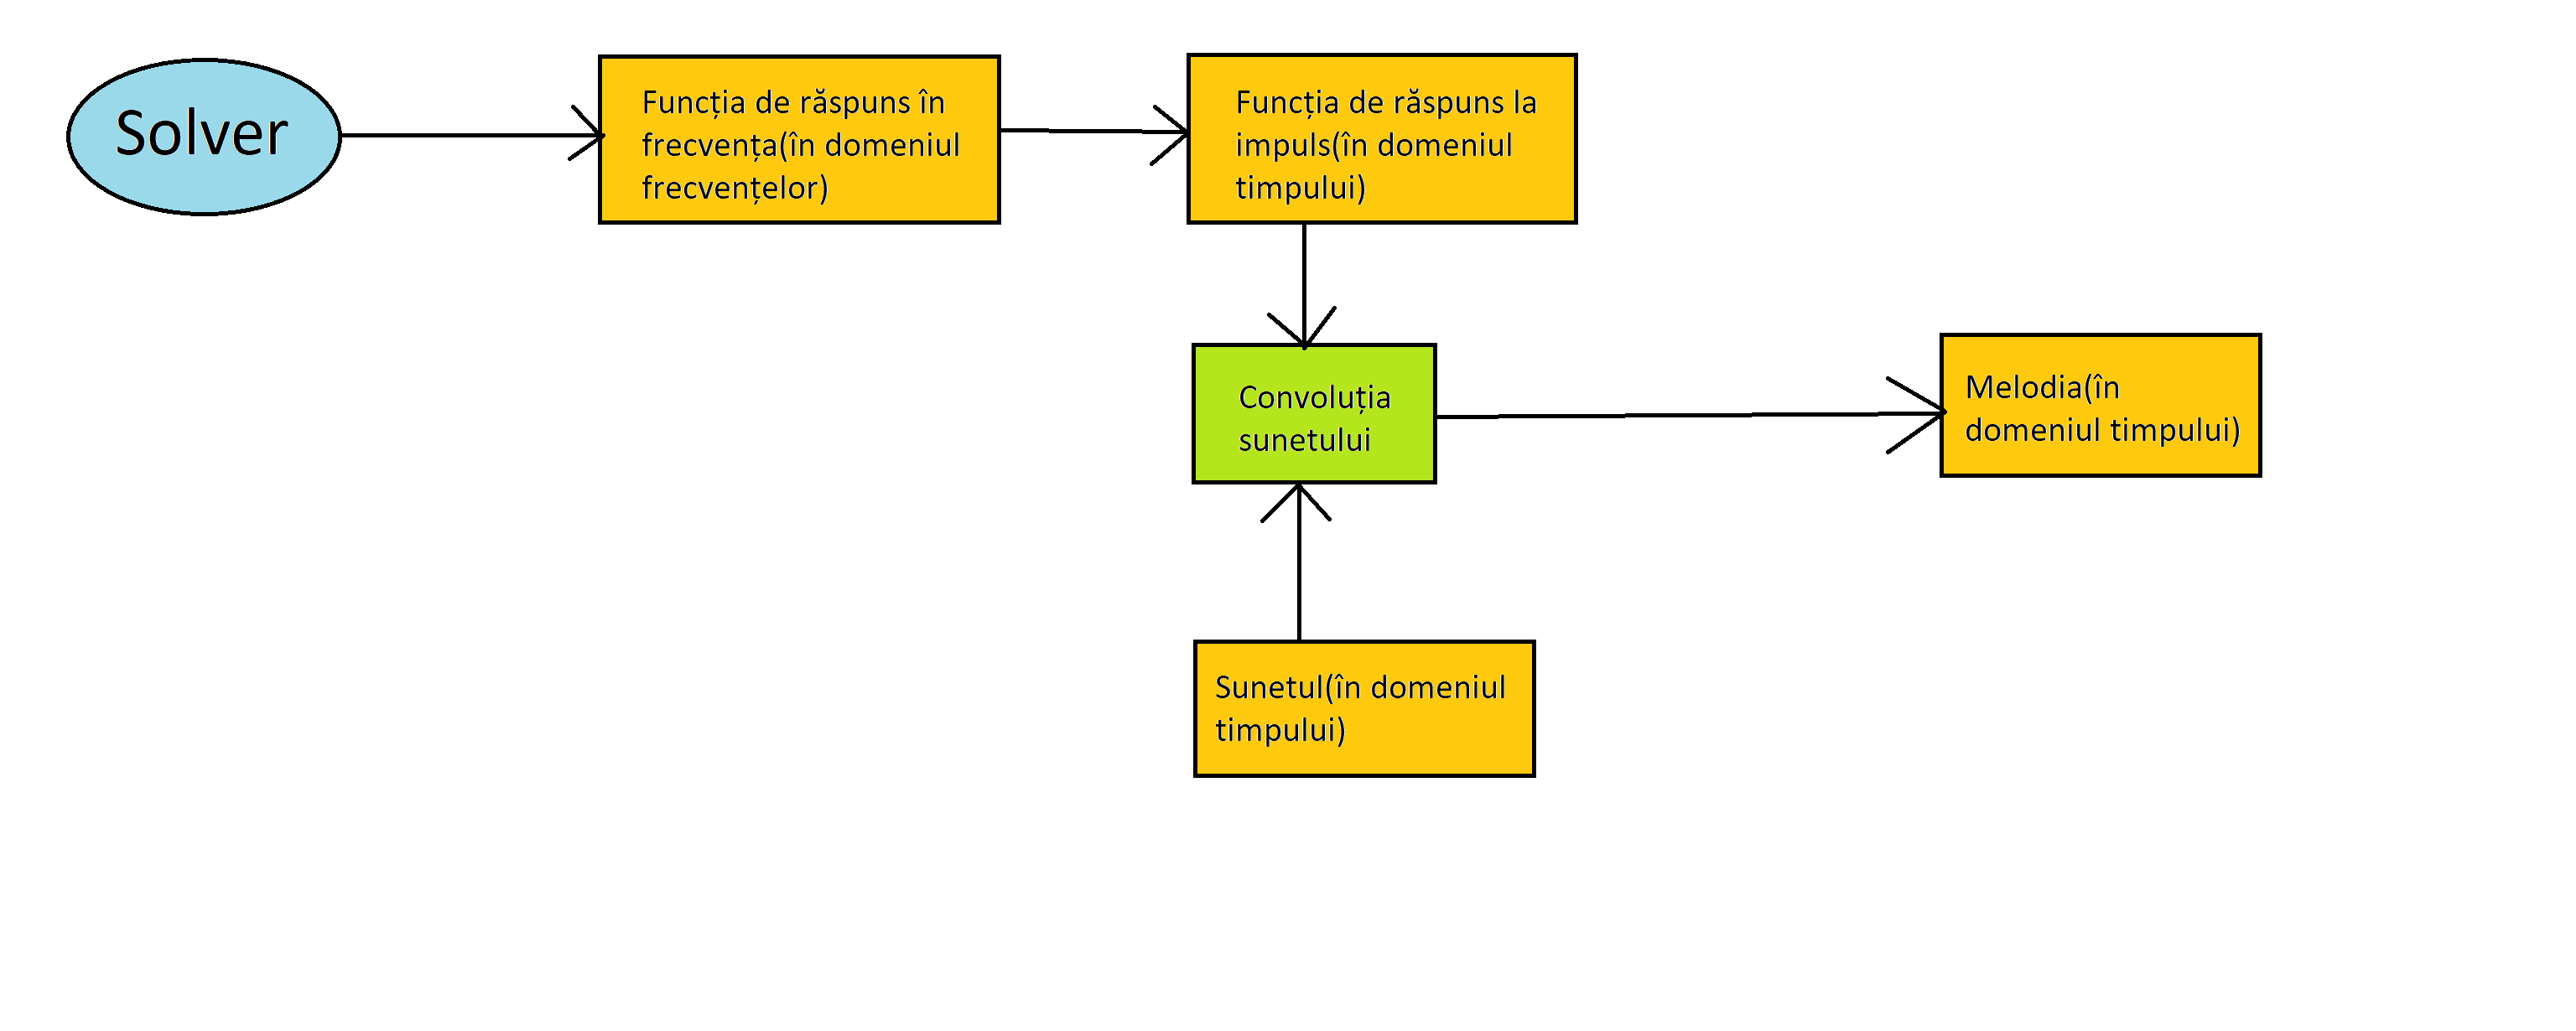
\includegraphics[width=18cm]{imagini/conv.png}
		\caption{Etapele parcurse pentru ob\c{t}inerea sunetului după convoluție}
		\label{Fig15}
	\end{figure}
	
	Func\c{t}ia de r\u{a}spuns la impuls se calculeaz\u{a} pe baza func\c{t}iei de r\u{a}spuns \^{i}n frecven\c{t}\u{a} cu ajutorul Inversei Transformatei Rapide Fourier care va permite trecerea de la domeniul frecven\c{t}elor la domeniul timpului pentru a preg\u{a}ti semnalul de intrare ca mai departe s\u{a} realiz\u{a}m convolu\c{t}ia sunetului.
	Ca s\u{a} putem trece mai departe \c{s}i s\u{a} calcul\u{a}m func\c{t}ia de r\u{a}spuns la impuls trebuie s\u{a} utiliz\u{a}m Algoritmul \ref{frResponse}.
	
	\begin{algorithm}
		\caption{Crearea func\c{t}iei de r\u{a}spuns \^{i}n frecven\c{t}\u{a}}
		\label{frResponse}
		\begin{algorithmic}[3]	
			\Procedure{\textit{r\u{a}spuns\_frecven\c{t}\u{a}}}{\textit{ecograme, microfoane, fr}}
			\State{\textit{r\u{a}spunsFr} $\gets$ dic\c{t}ionar gol}
			\For{$i \gets 0$ to $microfoane$}
			\State{$valori \gets$ list\u{a} numere complexe goal\u{a}}
			\For{$j \gets 0$ to $fr$}
			\State{$sum \gets \sum{ecograme[fr[j]][microfoane[i]]}$}
			\State{$valori.$\textit{adaug\u{a}($sum$)}}
			\EndFor
			\State{\textit{r\u{a}spunsFr[microfoane[i]]}$\gets valori$}
			\EndFor
			\EndProcedure
		\end{algorithmic}
	\end{algorithm}
	 
	
	Acum c\u{a} am ob\c{t}inut r\u{a}spunsul \^{i}n frecven\c{t}\u{a} putem trece la a calcula r\u{a}spunsul la impuls, iar acest lucru se poate face cu ajutorul IFFT, care va permite trecerea de la domeniul frecven\c{t}elor \^{i}napoi la domeniul timpului.
	
	\newpage
\subsection{Calculul distan\c{t}elor}

	Pentru a calcula distan\c{t}ele am folosit formula distan\c{t}ei lui Euler. Am considerat pentru fiecare raz\u{a}, toate punctele de coliziune \c{s}i am calculat lungimile pentru acestea iterativ.
	 
	
	\begin{equation}
		d(p_1, p_2) = \sqrt{(p_{1_x} - p_{2_x})^2 + (p_{1_y} - p_{2_y})^2 + (p_{1_z} - p_{2_z})^2}
	\end{equation}
	 
	
	Prin urmare, lungimea unei raze este calculat\u{a} astfel:
	\begin{equation}
		d_{razei} = \sum_{1}^{N-1}{d(p_i, p_{i+1})}
	\end{equation}
	unde $p_1, p_2, \dots, p_{N}$ sunt punctele de coliziune, iar $N$ reprezint\u{a} num\u{a}rul de puncte de coliziune.

\subsection{Calculul timpilor}

	Calculul timpilor implic\u{a} calculul lungimilor pentru fiecare raz\u{a} \c{s}i viteza sunetului, folosind urm\u{a}toarea formul\u{a}:
	\begin{equation}
		t = \frac{d}{c_{aer}}
	\end{equation}
	unde $t$ este timpul, $d$ reprezint\u{a} distan\c{t}a de la surs\u{a} p\^{a}n\u{a} la ultimul punct de coliziune al razei, iar $c_{aer}$ este viteza sunetului prin aer.

\section{Post-procesarea}

	Funcționalitatea de postprocesare modifică spectrul de frecvență al semnalului audio de intrare. Acest lucru va duce la creșterea anumitor benzi de frecvență, în timp ce altele sunt diminuate sau tăiate. Post-procesarea audio depinde de conținutul audio și presupune aplicarea unor filtre de cele mai multe ori. Post-procesarea audio conține patru mari categorii:
	
	\begin{itemize}
		\utb egalizatoare, care modifică frecvențele
		
		\utb controlul zgomotului, care se ocupă de variația sunetului semnalului audio
		
		\utb sunetul înconjurător, care se ocupă cu crearea unei scene audio realiste și direcționale
		
		\utb efecte audio de sistem, care se ocupă cu îmbunătățirea experienței de utilizare a playerului audio
	\end{itemize}

	Egalizatoarele pot fi utilizate pentru a compensa distorsiunile introduse de sistemul de difuzare a sunetului. Ele pot fi, de asemenea, utilizate pentru a modifica conținutul audio pentru a se potrivi preferințelor ascultătorului.
	
	Nivelul de sunet confortabil pentru conținutul audio depinde, în primul rând de nivelul de zgomotul din jur și, în al doilea rând, de conținutul în sine. În multe aplicații, proiectanții vor găsi necesitatea modificării intensității conținutului audio. Modulul de control al zgomotului măsoară și modifică în consecință intensitatea conținutului audio.

	Astfel, am ajuns \c{s}i la ultima etap\u{a} unde vom aplica opera\c{t}ii de post-procesare pentru a putea asculta sunetul pe microfoanele plasate \^{i}n \^{i}nc\u{a}pere. Astfel, la acest pas vom aplica un algoritm pentru convolu\c{t}ia sunetului ce va fi descris \^{i}n paginile ce urmeaz\u{a}.

\subsection{Convolu\c{t}ia sunetului}

	Convolu\c{t}ia sunetului se face pe baza func\c{t}iei de r\u{a}spuns la impuls. R\u{a}spunsul este alc\u{a}tuit dintr-o list\u{a} de valori reale care sunt transformate \^{i}ntr-un semnal discret. Convolu\c{t}ia presupune un sistem ce prime\c{s}te ca intrare un semanl \c{s}i pe care \^{i}l transform\u{a} pentru a ob\c{t}ine un semnal de ie\c{s}ire. \^{I}n cazul acestui model, semnalul de intrare este func\c{t}ia de r\u{a}spuns la impuls \c{s}i sunetul \^{i}n domeniul timpului, iar ie\c{s}irea este reprezentat\u{a} de valorile reale ale sunetului.
	  
	
	Teoria Fourier spune c\u{a} orice semnal digital poate fi exprimat ca o combina\c{t}ie de sinusoide, din acest motiv prefer\u{a}m s\u{a} realiz\u{a}m calculele \^{i}n domeniul frecven\c{t}elor (este mult mai rapid).
		
	\begin{figure}[!htb]
		\centering
		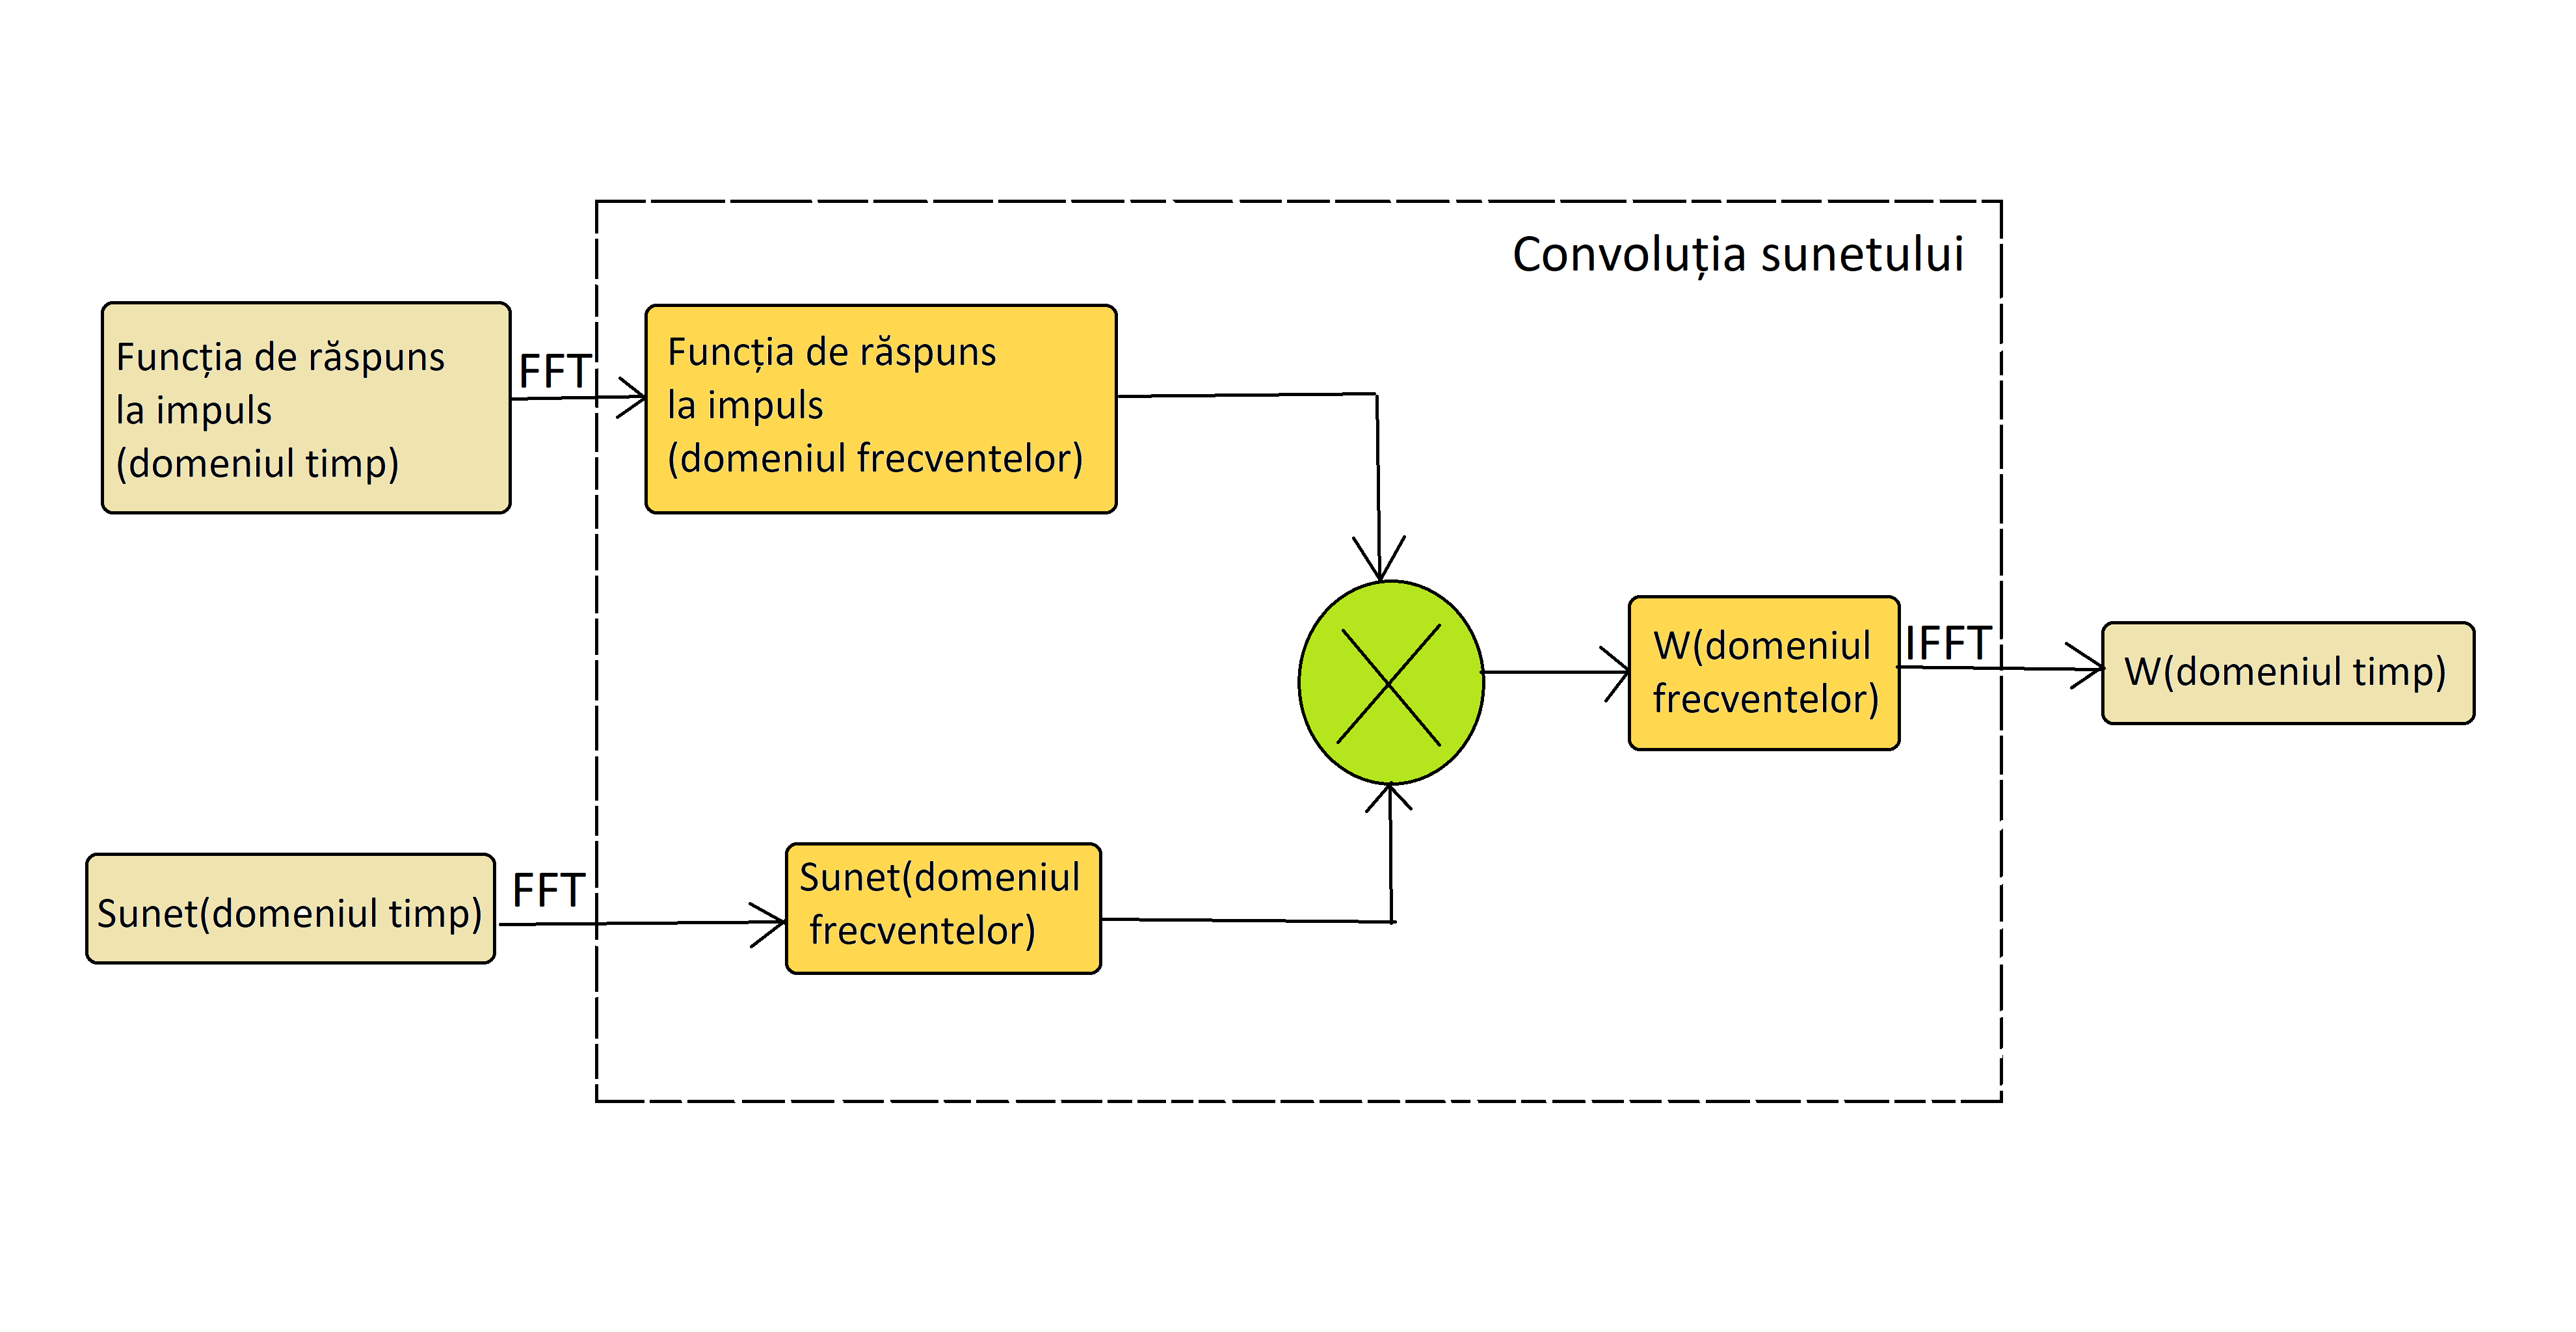
\includegraphics[width=15cm]{imagini/convolutiaSunetului.png}
		\caption{Etapele parcurse pentru convolu\c{t}ia sunetului}
		\label{Fig14}
	\end{figure}

	Precum este descris \c{s}i \^{i}n Figura \ref{Fig14}, convolu\c{t}ia sunetului preia ca intrare func\c{t}ia de r\u{a}spuns la impuls \c{s}i sunetul care a fost difuzat pe sursa audio. Aceste valori sunt \^{i}n domeniul timpului \c{s}i pentru a putea s\u{a} le aplic\u{a}m transform\u{a}rile trebuie s\u{a} trecem \^{i}n domeniul frecven\c{t}elor. Ob\c{t}inem astfel dou\u{a} polinoame ce trebuie \^{i}nmul\c{t}ite. R\u{a}spunsul ob\c{t}inut este \^{i}n domeniul frecven\c{t}elor \c{s}i pentru a calcula ie\c{s}irea trebuie s\u{a} trecem \^{i}napoi \^{i}n domeniul timpului cu ajutor Inversei Transformatei Rapide Fourier. Convolu\c{t}ia sunetului, tranform\u{a}rile din domeniul timpului \^{i}n domeniul frecven\c{t}elor \c{s}i invers au fost realizate cu ajutorul metodelor din NWaves: 
	
	\begin{itemize}
		\utb \textit{DiscreteSignal Operation.Convolve (DiscreteSignal signal, DiscreteSignal kernel);}
		
		\utb \textit{void RealFft.Inverse (float[] re, float[] im, float[] output);}
		
	\end{itemize}

	Semnalul de intrare este sunetul care va fi afectat, în timp ce răspunsul la impuls conține caracteristicile sonore ale spațiului sau obiectului pe care îl vom transmite semnalului de intrare.
	
	Un răspuns la impuls este creat prin redarea unui sunet sau a unui impuls într-un spațiu. Acest impuls poate fi: fie un sunet scurt (un pistol de pornire, un balon care se aprinde etc.), fie un sunet mai susținut ca o sinusoidală (un ton sinusoidal care se ridică prin spectrul de frecvență sonor). Acest impuls produce un instantaneu al ambianței caracteristice a spațiului în conformitate cu acustica unică a spațiului, o ambianță care poate fi capturată.
	
	Microfoanele sunt folosite pentru a înregistra sunetul rezultat. Având în vedere impulsul inițial, putem vedea cum acustica spațiului/obiectului afectează timbrul sunetului rezultat.
	
	În mod ideal, impulsul inițial ar fi editat din înregistrare, lăsând doar răspunsul acustic al spațiului. Acest lucru ar lăsa un semnal pur al spațiului, mai degrabă decât să includă un alt sunet cu spațiul.
	
	În esență, convoluția este procesul de multiplicare a spectrelor de frecvență ale celor două surse audio - semnalul de intrare și răspunsul la impuls. Procedând astfel, frecvențele care sunt partajate între cele două surse vor fi accentuate, în timp ce frecvențele care nu sunt partajate vor fi atenuate. Acesta este motivul pentru care semnalul de intrare capătă calitățile sonore ale răspunsului la impuls, deoarece frecvențele caracteristice din răspunsul la impuls comun în semnalul de intrare sunt amplificate.

	Procedura este semnificativ mai eficientă din punct de vedere al timpului de calcul decât celelalte două etape, deoarece folosind Transformata Fourier Rapidă (FFT) ajungem la $n\log_2n$ operații necesare pentru a realiza convoluția sunetului.	
	\chapter{Testarea \c{s}i analizarea rezultatelor}
		\section{Realizarea experimentelor și analizarea acestora}

	Pentru a putea testa și analiza rezultatele obținute folosind modelul acustic propus de această lucrare am creat o modalitate interactivă pentru a putea vizualiza și compara rezultatele obținute de modelul nostru folosind platforma Unity pentru a gestiona și dezvolta un software de simulare acustică folosind un game engine. Am construit trei încăperi, două dreptunghiulare și una sferică, pornind de la forme de bază și materiale contrastante pentru a putea facilita vizualizarea rezultatelor. 
	
	În cadrul experimentelor realizate au fost folosite următoarele spații interioare 3D:
	
	\begin{itemize}
		\utb Cameră rectangulară cu dimensiunile: 4m lățime, 5m lungime și 3m înălțime - Camera 1 
		
		\utb Cameră rectangulară cu dimensiunile: 30m lățime, 30m lungime și 15m înălțime - Camera 2 
		
		\utb Cameră sferică cu raza egală cu 5m - Camera 3 
	\end{itemize}

	Această serie de experimente ia în considerare mai mulți parametrii esențiali în contextul modelului acustic, precum: numărul de raze ce va fi distribuit în încăpere, numărul maxim de reflexii pe care o rază le poate atinge, lungimea maximă pe care o poate avea o rază și pasul de frecvență.	
	
	În această lucrare vom considera următoarea serie de notații:
	\begin{itemize}
		\utb $S$ - sursă audio
		
		\utb $M$ - microfon 
	\end{itemize}

	Atunci când discutăm despre un punct în spațiu am considerat un sistem de coordonate în trei dimensiuni $(x,y,z)$, unde $x$ este axa ce reprezintă lungimea, $y$ este înălțimea, iar $z$ este lățimea.
	
	Pentru ca experimentele să fie relevante am considerat aceeași configurație și aceeași melodie ce va fi difuzată pentru toate încăperile. Configurația folosită va fi:
	
	\begin{itemize}
		\utb 100 000 de raze distribuite uniform pentru camerele dreptunghiulare și 10 000 în cazul încăperii sferice
		
		\utb maxim 10 reflexii pentru o rază
		
		\utb 200m distanța maximă pe care o rază o poate parcurge
		
		\utb 8192Hz numărul de pași de frecvență
	\end{itemize}

	Pentru rularea modelului acustic este nevoie să considerăm o serie de microfoane, întrucât dorim să analizăm sunetul în anumite poziții ale încăperilor. Astfel, în Camera 1 am considerat poziția sursei $S(0, 0, 0)$ și următoarele poziții pentru microfoane:
	
	\begin{itemize}
		\utb $M0(2, 1.6, 1.7)$, fiind la distanța de 3.07m de sursă
		
		\utb $M1(-1.5, 1.2, 1.7)$, fiind la distanța de 2.56m de sursă
		
	\end{itemize}

	În Camera 2, sursa $S$ se află la poziția $S(0, 2.5, 0)$ și am considerat următoarele valori pentru pozițiile microfoanelor: 
	
	\begin{itemize}
		\utb $M0(2, 1.6, 1.7)$, fiind la distanța de 3.07m de sursă
		
		\utb $M1(-1.5, 1.2, 1.7)$, fiind la distanța de 2.56m de sursă
		
		\utb $M2(1, 2, 13)$, fiind la distanța de 13.19m de sursă
	\end{itemize}

	Pentru Camera 3, sursa $S$ este poziționată în punctul $S(0, 0, 4)$. Am utilizat ecuația Cercului pentru a putea împrăștia uniform microfoanele în încăpere, obținând astfel următoarele valori pentru pozițiile microfoanelor:
	
	\begin{itemize}
		\utb $M0(4, 0, 0)$, fiind la distanța de 5.65m de sursă
		
		\utb $M1(2.8284, 0, 2.8284)$, fiind la distanța de 3.06m de sursă
		
		\utb $M2(-2.8284, 0, 2.8284)$, fiind la distanța de 3.06m de sursă
		
		\utb $M3(-4, 0, 4.8984)$, fiind la distanța de 4.09m de sursă
		
		\utb $M4(-2.8284, 0, -2.8284)$, fiind la distanța de 7.39m de sursă
		
		\utb $M5(-7.347, 0, -4)$, fiind la distanța de 10.86m de sursă
		
		\utb $M6(2.8284, 0, -2.8284)$, fiind la distanța de 7.39m de sursă
	\end{itemize}


	Mediul în care trăim conține suprafețe și materiale, care absorb sau reflectă sunetul, fapt care atenuează sau împrăștie ceea ce noi auzim. Posibilitatea de a întâłni suprafețe care să absoarbă sau să reflecte total sunetul este una foarte mică, de obicei, acest lucru se întâmplă doar în condiții de laborator. 
	
	În funcție de suprafețe, coeficientul de absorbție diferă foarte mult, de obicei, obiecte precum covoarele, pânzele, pernele, absorb sunetul mult mai bine decât materiale precum lemnul, betonul, poliesterul. Astfel, am dorit ca soluția modelului acustic să fie una cât mai realistă și am considerat pentru toate suprafețele din încăperi o serie de coeficienți de absorbție. În cadrul experimentelor realizate, am ales coeficientul de absorbție 0.2.

	În Figura \ref{fig:Fig20} putem vizualiza cele trei încăperi, microfoanele și sursa audio realizate cu ajutorul platformei Unity. Se poate observa că prima încăpere este mai mică decât cea de-a doua și că cele două spații sunt similare. Pentru Camera 3, se consideră distribuirea uniformă a microfoanelor folosind ecuația cercului.
	
	\begin{figure}[!htb]%
		\begin{subfigure}[b]{.3\textwidth}
			\centering
			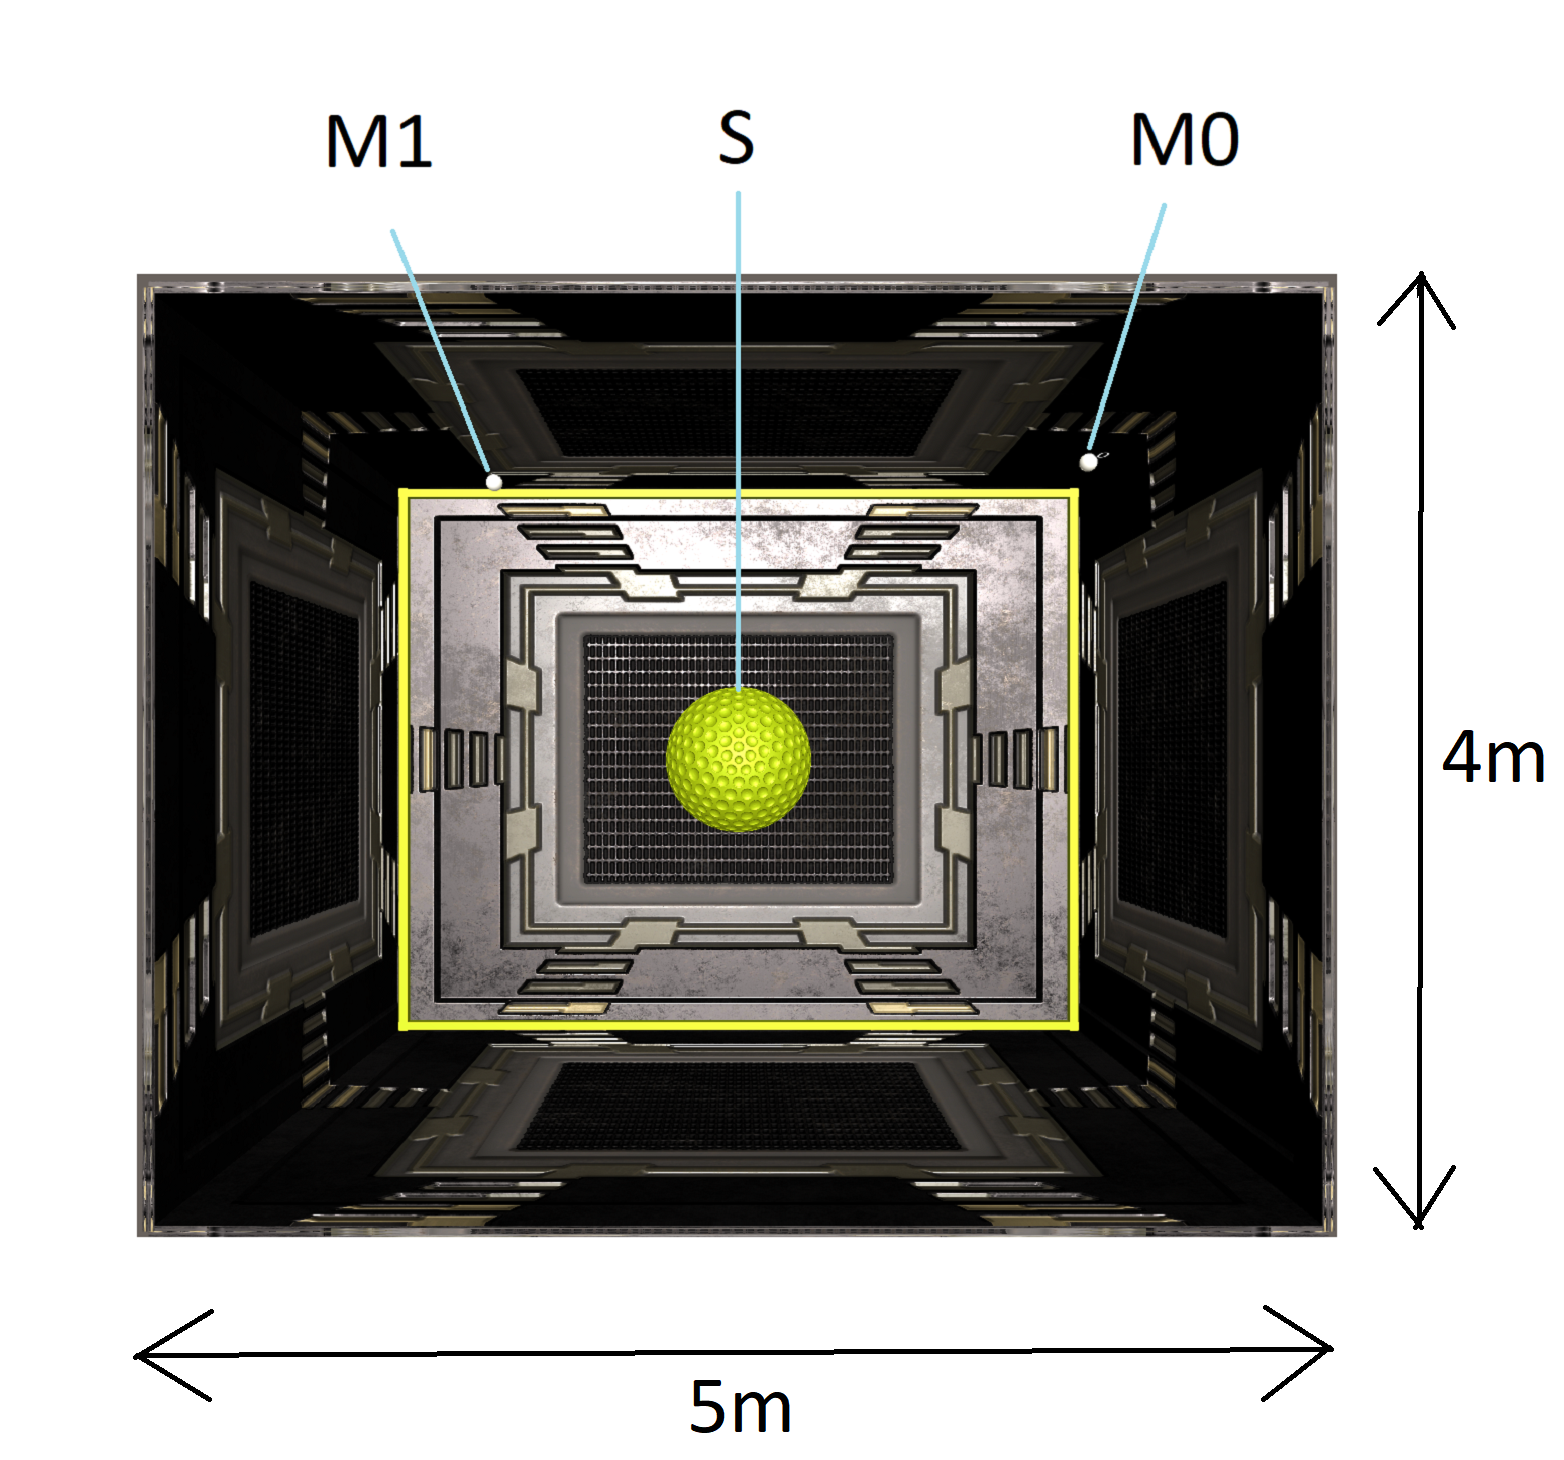
\includegraphics[width=1\linewidth]{imagini/roomA.png} 
			\caption{Camera 1}
			\label{fig:sub-fig}
		\end{subfigure}
		\hfill
		\begin{subfigure}[b]{.3\textwidth}
			\centering
			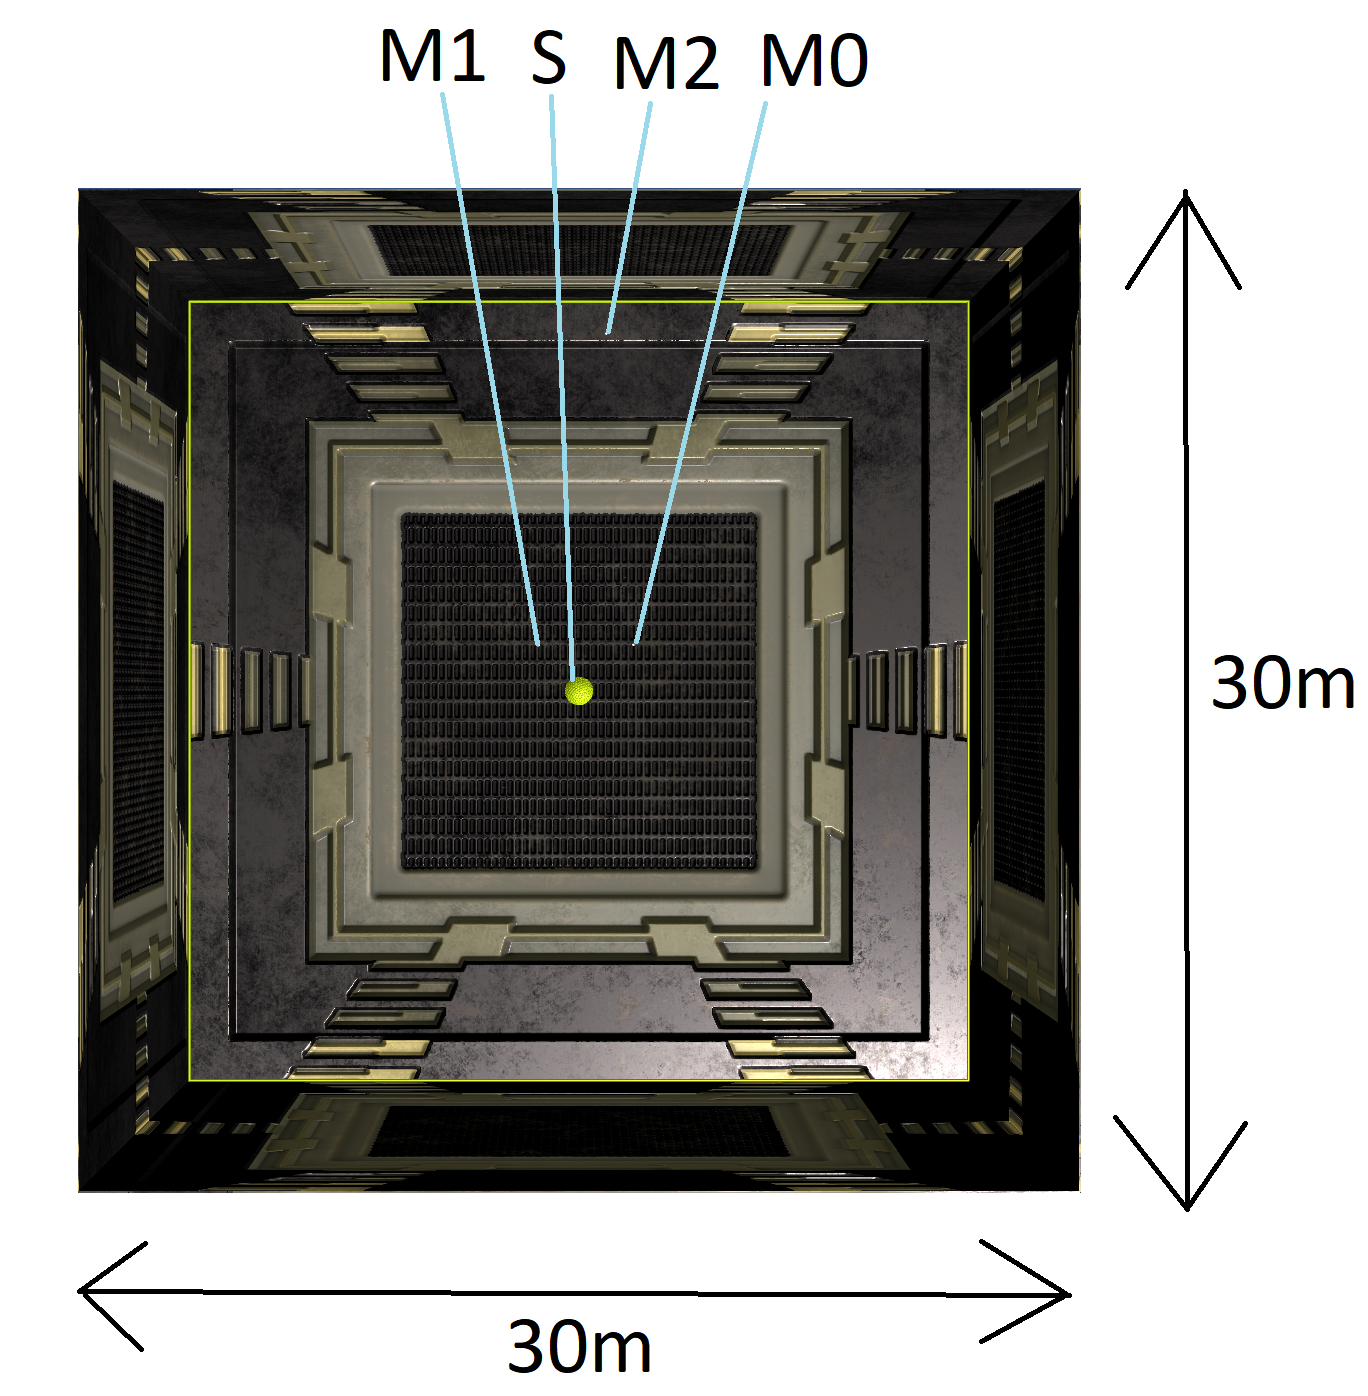
\includegraphics[width=1\linewidth]{imagini/roomB.png}
			\caption{Camera 2}
			\label{fig:sub-second}
		\end{subfigure}
		\hfill
		\begin{subfigure}[b]{.3\textwidth}
			\centering
			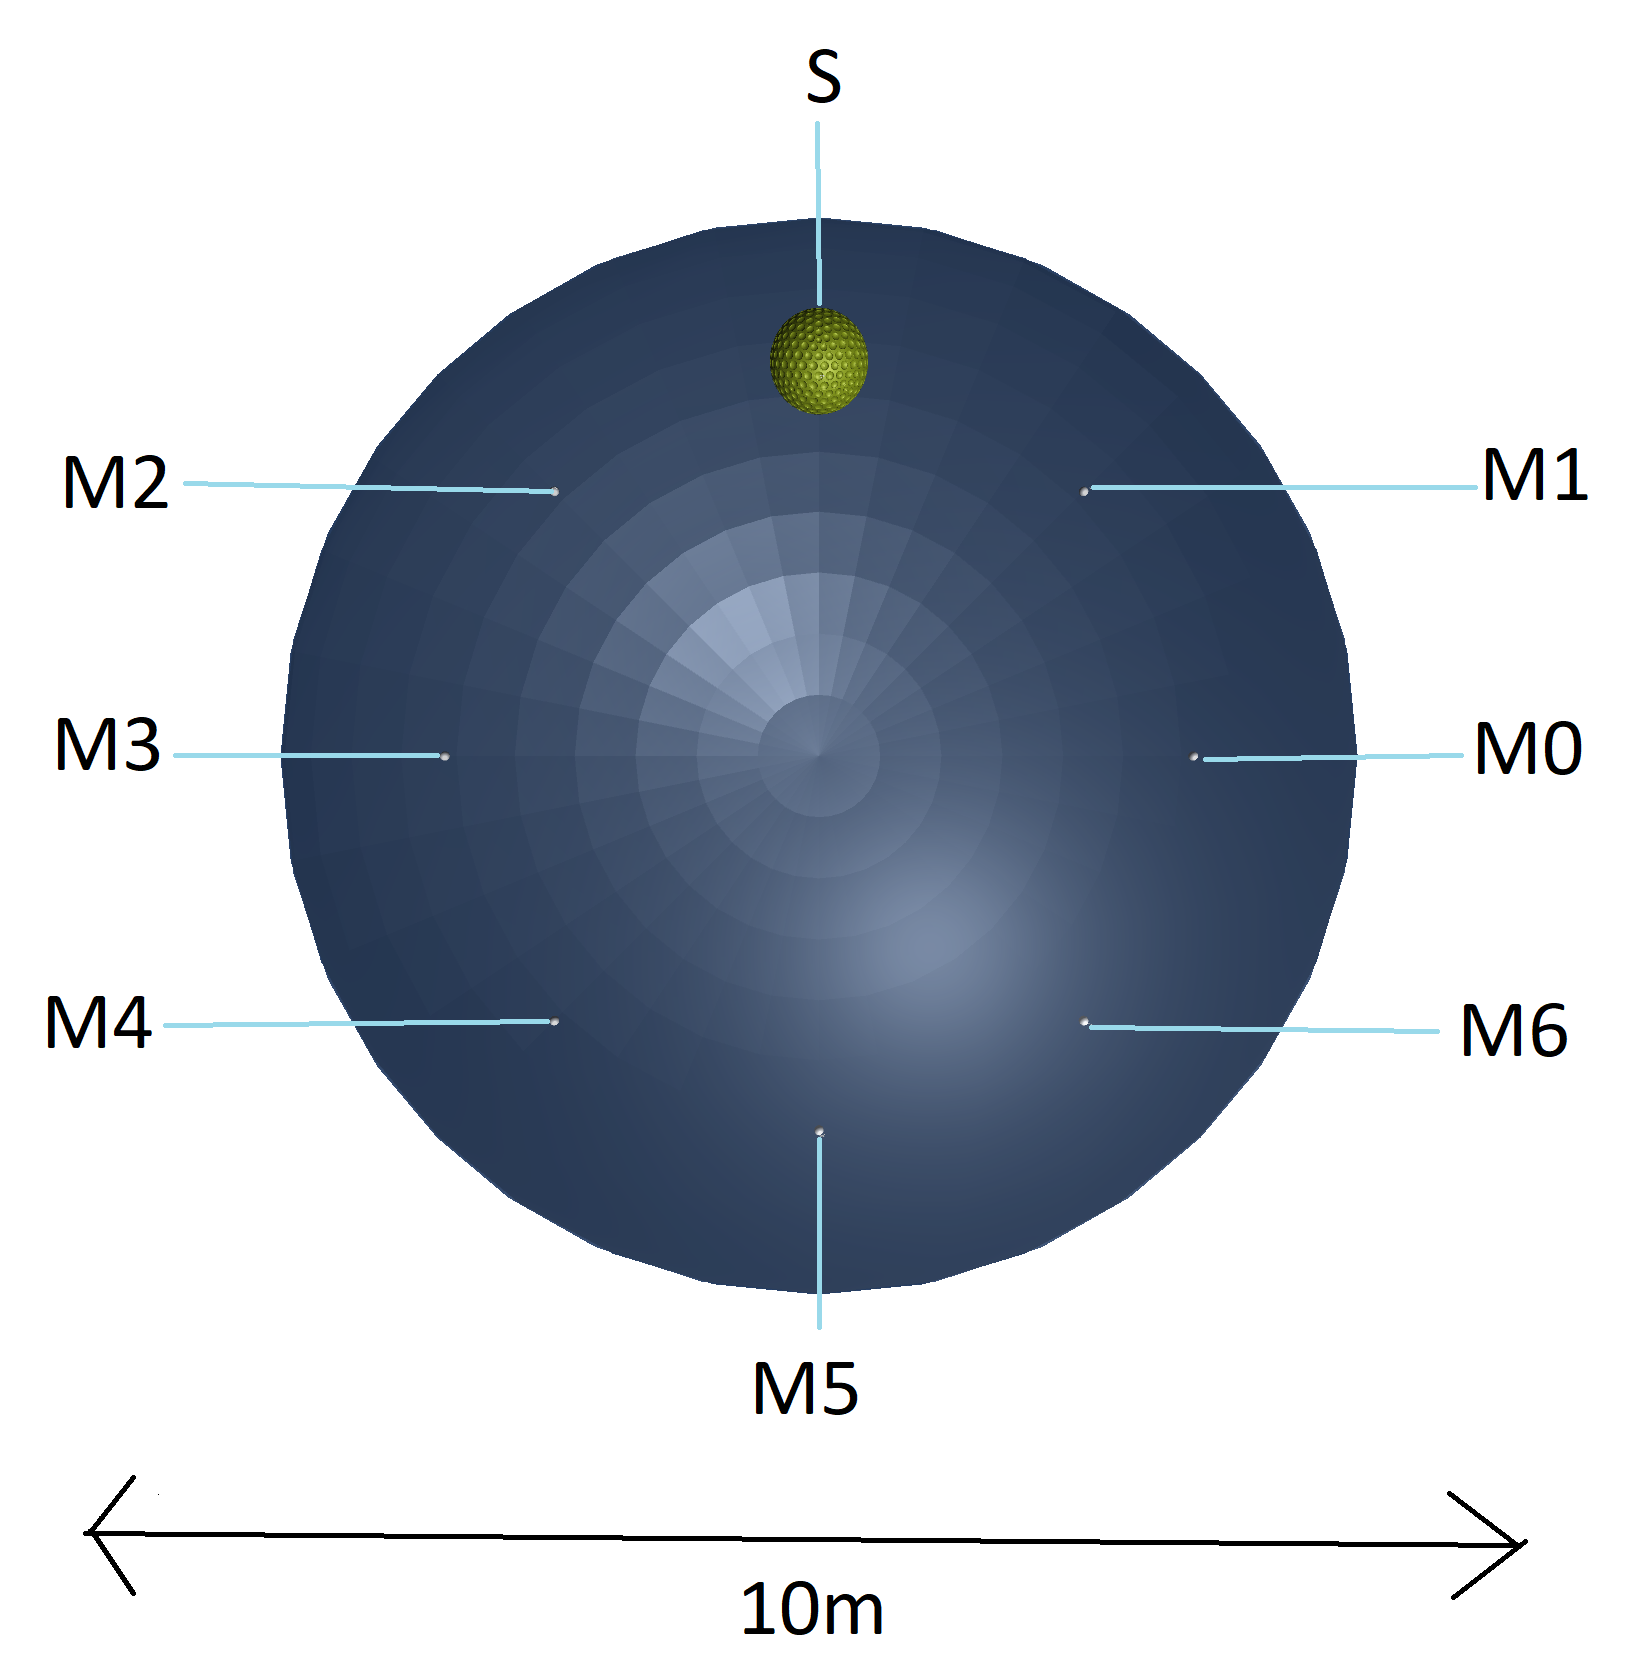
\includegraphics[width=1\linewidth]{imagini/roomC.png}
			\caption{Camera 3}
			\label{fig:sub-third3}
		\end{subfigure}
		
		\caption{Încăperile folosite pentru a realiza experimentele}
		\label{fig:Fig20}
	\end{figure}
	
	Putem observa în cazul Subfigurii \ref{fig:sub-fig} că datorită configurației potrivite este acoperită cea mai mare parte din suprafața încăperii, nefiind prezente ,,spații goale'', semn care indică faptul că sunetul a fost împrăștiat în toată camera și că poate fi auzit peste tot.
	
	Subigura \ref{fig:sub-second} ilustrează cea de-a doua încăpere și razele ce au fost distribuite în aceasta. Datorită configurației alese și a pozițiilor microfoanelor putem observa că multe porțiuni ale camerei au rămas neparcurse.
	
	În Subfigura \ref{fig:sub-third3} putem observa că datorită configurației potrivite și al modului simetric în care au fost plasate microfoanele razele au fost împrăștiate în încăpere în mod uniform.
	
	Figura \ref{fig:Fig21} prezintă unul din modurile de vizualizare al razelor din aplicație. În aceste imagini a fost utilizată configurația parametrilor, poziționarea microfoanelor și a sursei audio prezentate mai sus. 

	\begin{figure}[!htb]%
		\begin{subfigure}[b]{.3\textwidth}
			\centering
			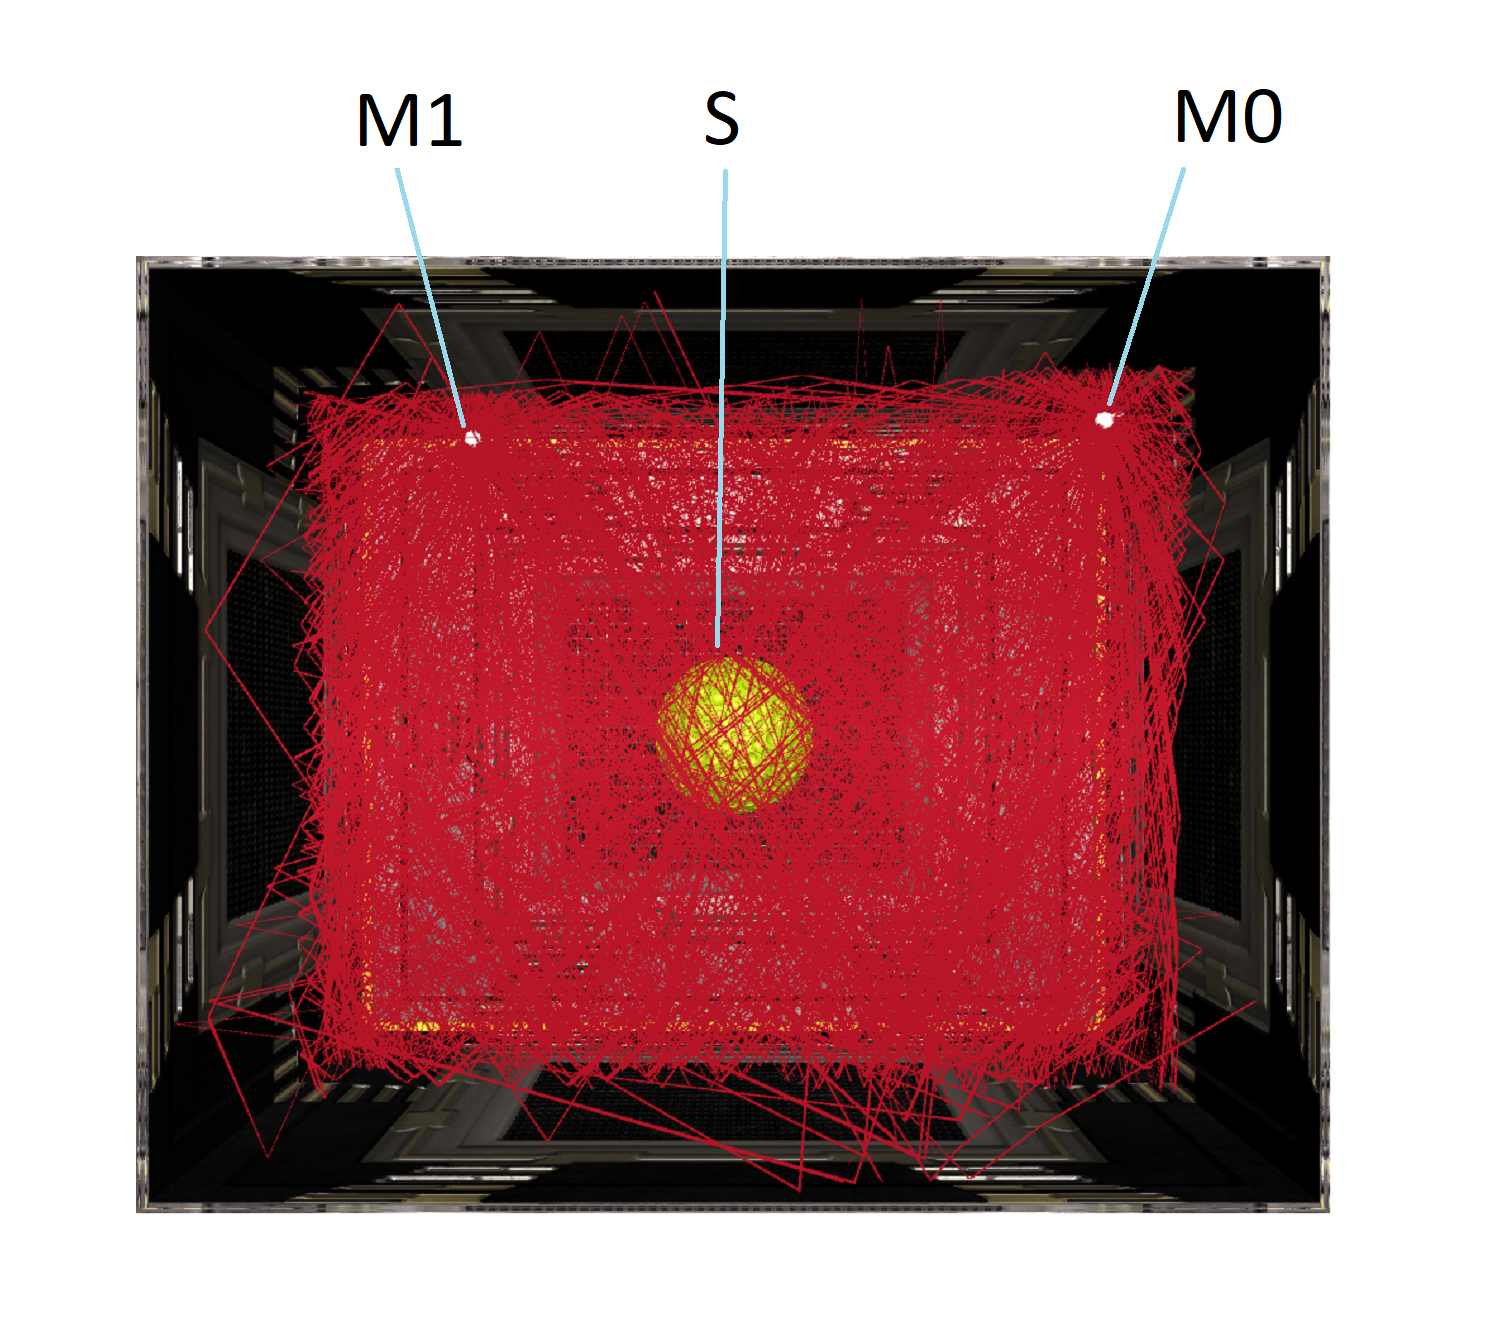
\includegraphics[width=1\linewidth]{imagini/roomA_rays.png} 
			\caption{Camera 1}
			%\label{fig:sub-fig}
		\end{subfigure}
		\hfill
		\begin{subfigure}[b]{.3\textwidth}
			\centering
			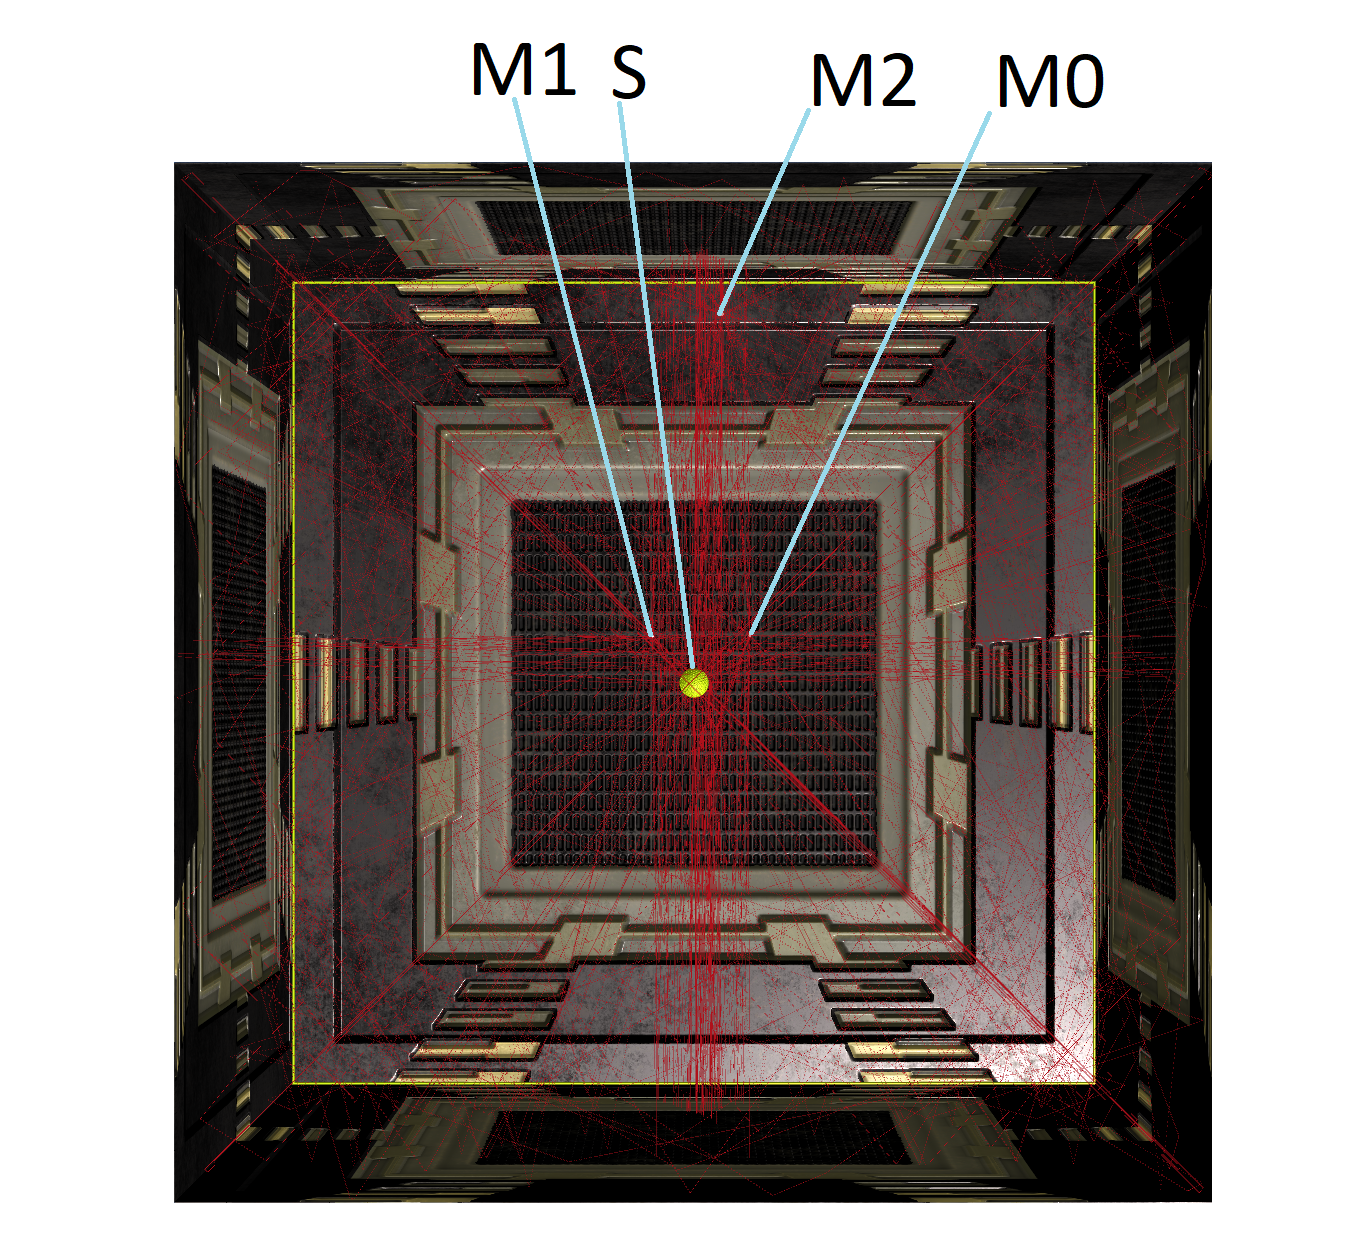
\includegraphics[width=1\linewidth]{imagini/roomB_rays.png}
			\caption{Camera 2}
			%\label{fig:sub-second}
		\end{subfigure}
		\hfill
		\begin{subfigure}[b]{.3\textwidth}
			\centering
			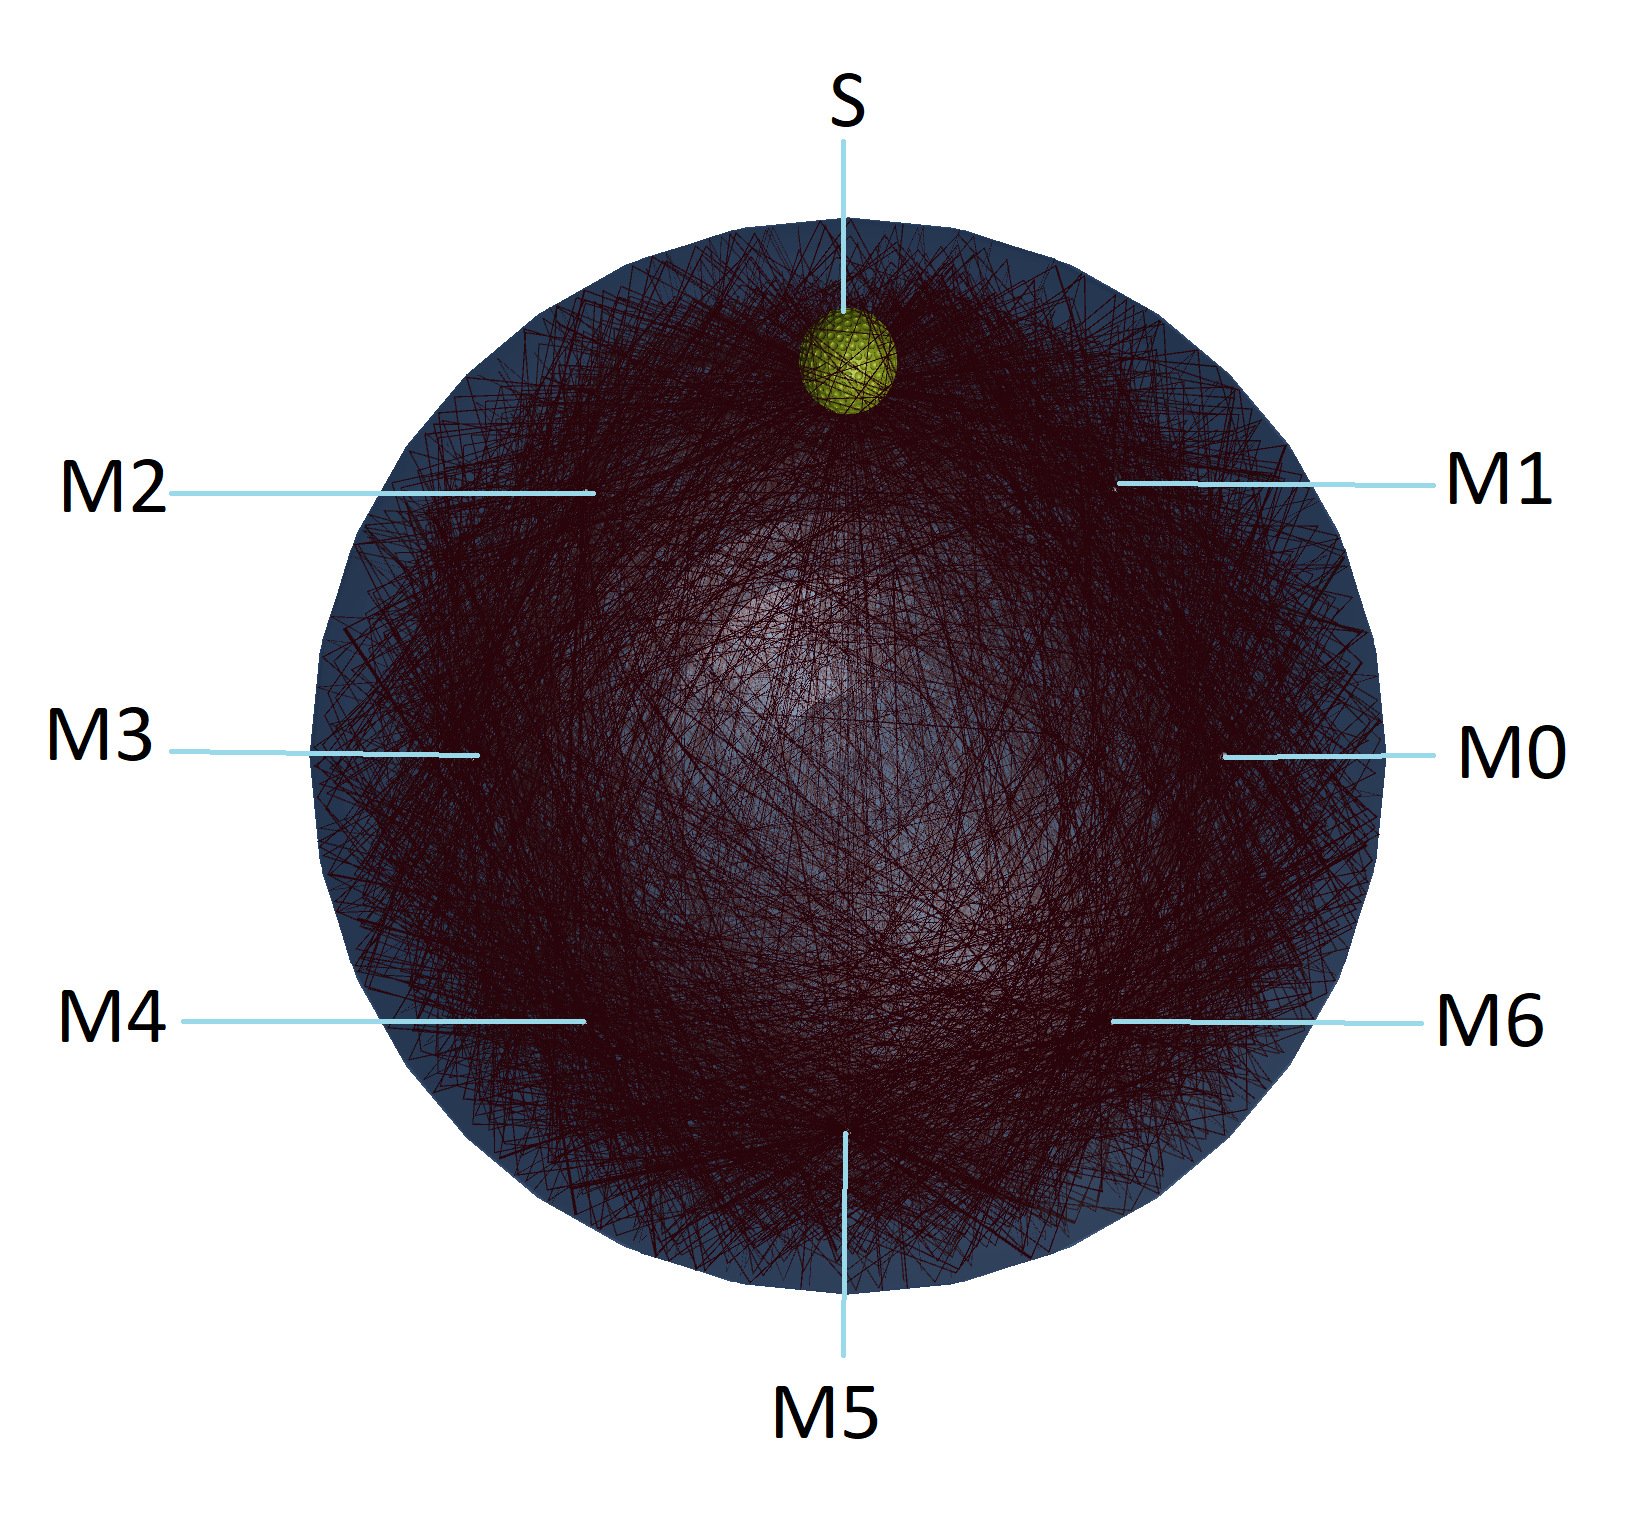
\includegraphics[width=1\linewidth]{imagini/roomC_rays.png}
			\caption{Camera 3}
			\label{fig:sub-third}
		\end{subfigure}
		
		\caption{Vizualizarea tuturor razelor din fiecare încăpere}
		\label{fig:Fig21}
	\end{figure}

	De asemenea, am realizat și un experiment în Camera 3 care presupune plasarea unui obstacol sferic între microfoanele $M4$ și $M5$ pentru a putea vedea dacă în acest mod sunt afectate rezultatele folosind modelul acustic. Pentru model am considerat aceeași configurație ca cea pentru Camera 1 și Camera 2, cu diferența că în încăperea sferică am considerat numărul de raze egal cu 10 000. În urma calculelor efectuate, am descoperit că 442 de raze au ajuns, în total, pe microfoane în cazul expus de Subfigura \ref{fig:sub-third} și
	378 în cazul expus de Subfigura \ref{fig:sub-third2}. Mai mult, am observat că, în cazul în care avem un obstacol în cameră, razele sunt
	mai împrăștiate și că anumite porțiuni nu sunt atât de dense, deoarece datorită obstacolului sunt create noi căi de propagare.
	
	Pe baza situațiilor prezentate mai sus putem vedea că în cazul încăperilor dreptunghiulare pe colțurile camerelor razele ajung mai greu, în timp ce în cazul încăperilor sferice razele ajung mai greu la centrul sferei.
	
	Dacă numărul de raze va fi prea mic în comparație cu dimensiunea camerei noastre, nu vom putea propaga sunetul foarte bine, deoarece există posibilitatea ca foarte puține raze sau chiar nici una să ajungă pe unul dintre microfoanele plasate în cameră. Deci, cu cât dimensiunea camerei este mai mare, cu atât este mai mare numărul de raze care vor fi distribuite în cameră și același lucru se întâmplă pentru numărul de reflexii și pentru lungimea maximă posibilă a unei raze.
	
	\begin{figure}[!htb]%
		\begin{subfigure}[b]{.3\textwidth}
			\centering
			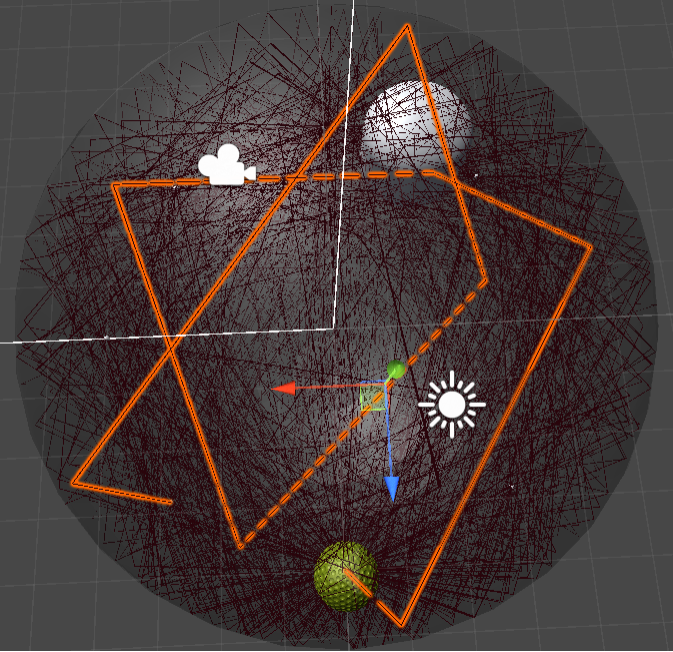
\includegraphics[width=1\linewidth]{imagini/m1r22-5000.png} 
			\caption{Raza trece pe deasupra, dar și lovește obstacolul}
			%\label{fig:sub-fig}
		\end{subfigure}
		\hfill
		\begin{subfigure}[b]{.3\textwidth}
			\centering
			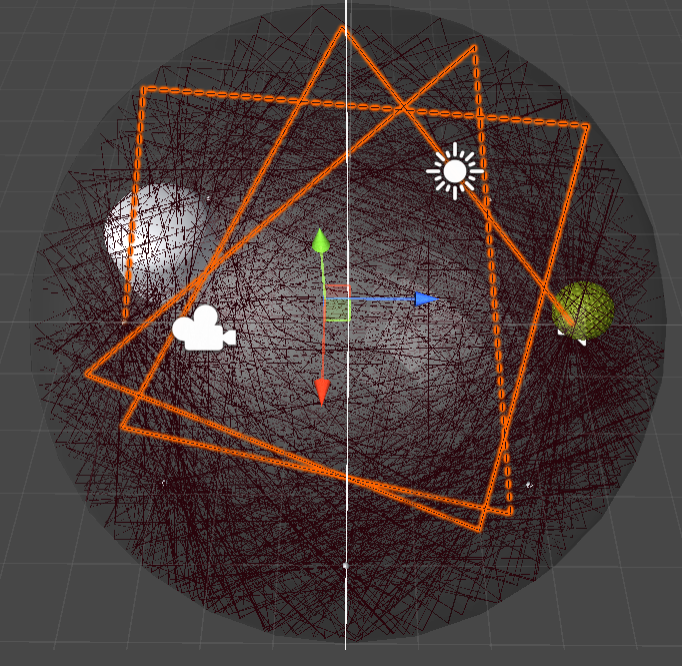
\includegraphics[width=1\linewidth]{imagini/m6r135-5000.png}
			\caption{Raza nu lovește deloc obstacolul}
			%\label{fig:sub-second}
		\end{subfigure}
		\hfill
		\begin{subfigure}[b]{.3\textwidth}
			\centering
			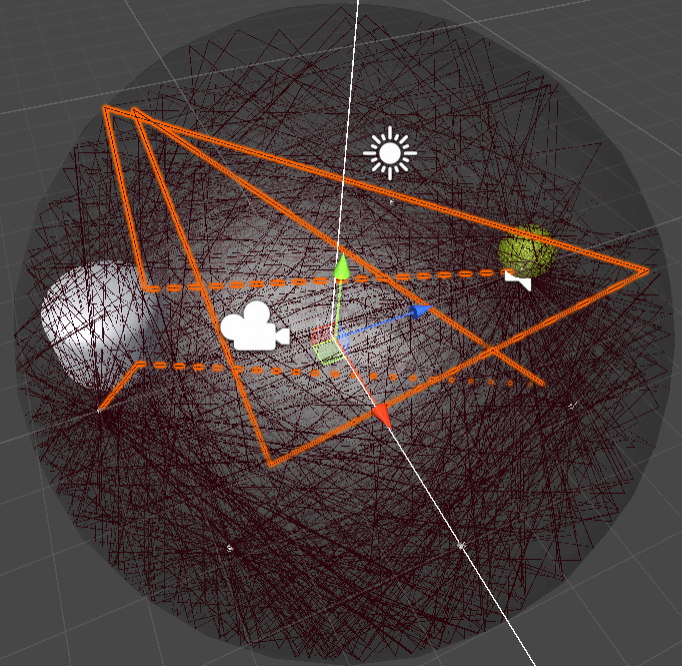
\includegraphics[width=1\linewidth]{imagini/m6r124-5000.png}
			\caption{Raza lovește de mai multe ori obstacolul}
			\label{fig:sub-third2}
		\end{subfigure}
		
		\caption{Diferite scenarii ale razelor}
		\label{fig:Fig22}
		
	\end{figure}

	Urmărind Figura \ref{fig:Fig22} putem observa că atunci când plasăm un obstacol în încăpere putem să ne aflăm în una dintre următoarele situații atunci când discutăm despre calea pe care o rază o parcurge: raza poate lovi sau nu obstacolul, poate trece pe deasupra sau pe dedesubtul acestuia.
	
	\begin{figure}[!htb]
		\centering
		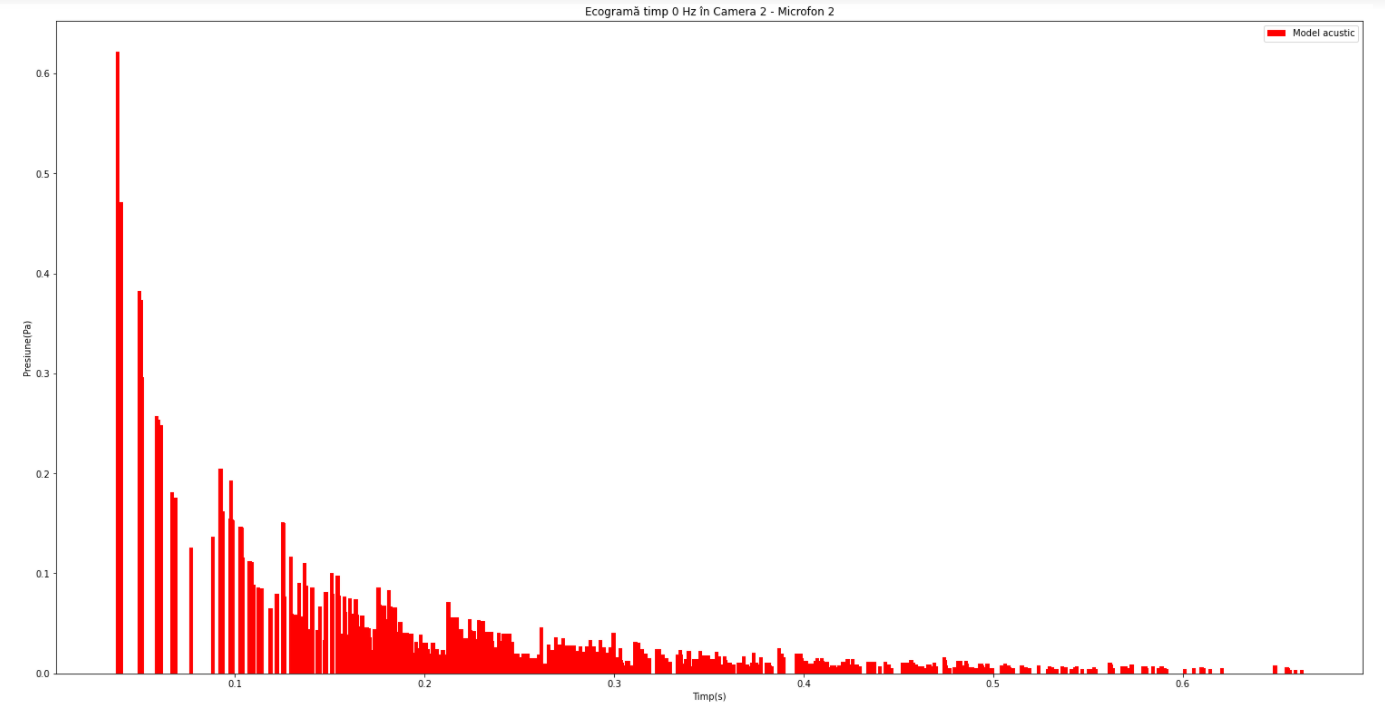
\includegraphics[width=1\linewidth]{imagini/ecograma.png}
		\caption{Ecogramă timp pe microfonul $M2$ în Camera 2}
		\label{Fig23}
	\end{figure}
	
	Considerând aceste cazuri de propagare al razelor în încăperea sferică putem trage concluzia că razele pot avea căi foarte diferite de a ajunge la microfon și că atunci când distanța unei raze de la sursa audio la microfon este foarte mare și sunetul va ajunge mai târziu.
	
	Atunci când discutăm despre ecograma în timp a unui microfon ne vom referi la graficul ce descrie presiunea și timpul. Se poate observa că Figura \ref{Fig23} conține o serie de bare verticale, unde fiecare bară reprezintă una dintre razele ce au ajuns pe microfonul 2 în Camera 2. Prima bară se caracterizează printr-o presiune crescută, deoarece corespunde razei care ajunge de pe sursă pe microfon în mod direct, fără a mai lovi alte suprafețe din încăpere. După această rază, urmează toate celelalte raze care au ajuns pe microfonul 2. Ordinea va fi dată de către numărul de reflexii și de către momentul în care raza ajunge pe microfon. Astfel, vom avea mai întâi raza directă, iar mai apoi razele care au o reflexie, după aceea două și așa mai departe până ajungem la raze ce au 10 reflexii.

	\begin{figure}[!htb]%
		\begin{subfigure}[b]{0.95\textwidth}
			\centering
			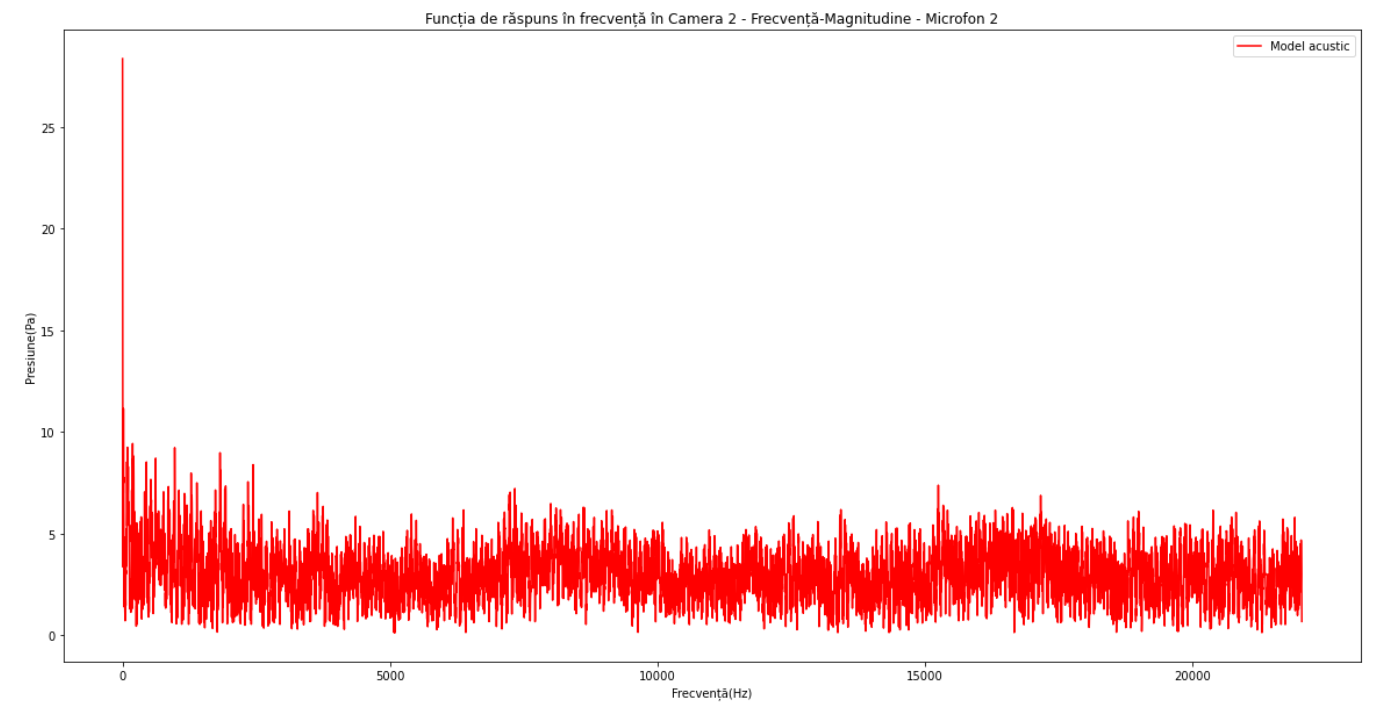
\includegraphics[width=1\linewidth]{imagini/fr_mag.png} 
			\caption{Grafic Frecvență-Magnitudine pe microfonul $M2$ în Camera 2}
			%\label{fig:sub-fig}
		\end{subfigure}
		\vfill
		\begin{subfigure}[b]{0.95\textwidth}
			\centering
			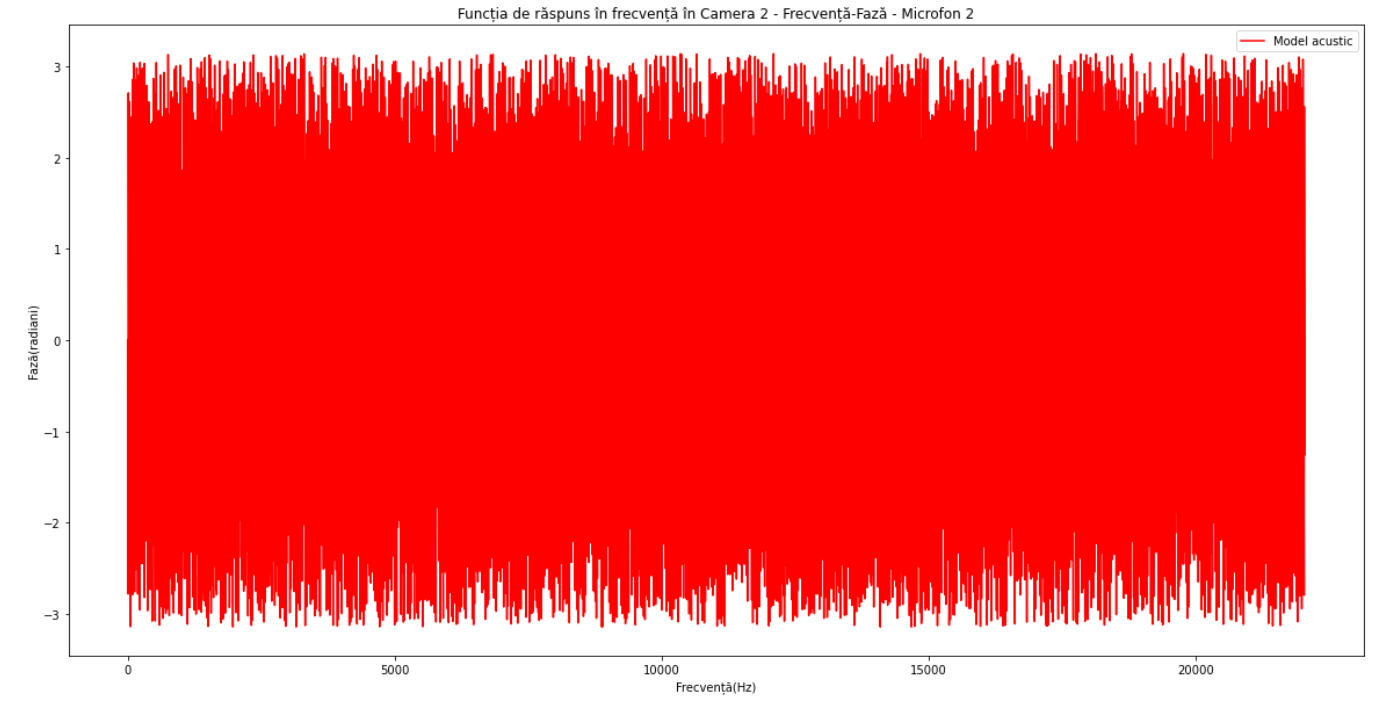
\includegraphics[width=1\linewidth]{imagini/fr_faza.png}
			\caption{Grafic Frecvență-Fază pe microfonul $M2$ în Camera 2}
			%\label{fig:sub-second}
		\end{subfigure}
		
		\caption{Funcția de răspuns în frecvență pe microfonul $M2$ în Camera 2}
		\label{fig:Fig24}	
	\end{figure}

	Funcția de răspuns în frecvență este măsura cantitativă a spectrului de ieșire al unui sistem sau dispozitiv ca răspuns la un stimul și este utilizat pentru a caracteriza dinamica sistemului. În termeni simpli, dacă o undă sinusoidală este injectată într-un sistem la o frecvență dată, un sistem liniar va răspunde la aceeași frecvență cu o anumită magnitudine și un anumit unghi de fază relativ la intrare.
	
	Funcția de răspuns în frecvență are, în general, valori complexe, cu părți reale și imaginare. Acest lucru este adesea mai util și mai intuitiv atunci când este exprimat în coordonate polare. Adică îl putem separa în magnitudinea sa (numită răspuns de amplitudine) și în
	componentă de fază (numită răspuns de fază).
	
	Reprezentarea domeniului de frecvență al unui semnal conține informații despre magnitudinea și faza semnalului la fiecare frecvență. Acesta este motivul pentru care ieșirea calculului FFT (Fast Fourier Transform) este complexă. Ieșirea FFT este un vector complex care conține informații despre conținutul de frecvență al semnalului. Faza prezintă modul în care se aliniază componentele de frecvență în timp. Aceste lucruri pot fi vizualizate în Figura \ref{fig:Fig24}, în cazul microfonului 2 din Camera 2.

	În procesarea semnalului, un răspuns la impuls este ieșirea unui sistem atunci când alimentăm sistemul cu un impuls ca semnal de intrare. Un impuls este orice semnal de scurtă durată. Cu toate acestea, în procesarea semnalului folosim, de obicei, o funcție Dirac Delta pentru sistemele analogice/continue. Pentru microfonul 2 din Camera 2 am obținut funcția de răspuns la impuls prezentată în Figura \ref{ir}, unde putem observa suișuri și coborâșuri ce ilsutrează fenomenul de ecou. 
	
	\begin{figure}[!htb]
		\centering
		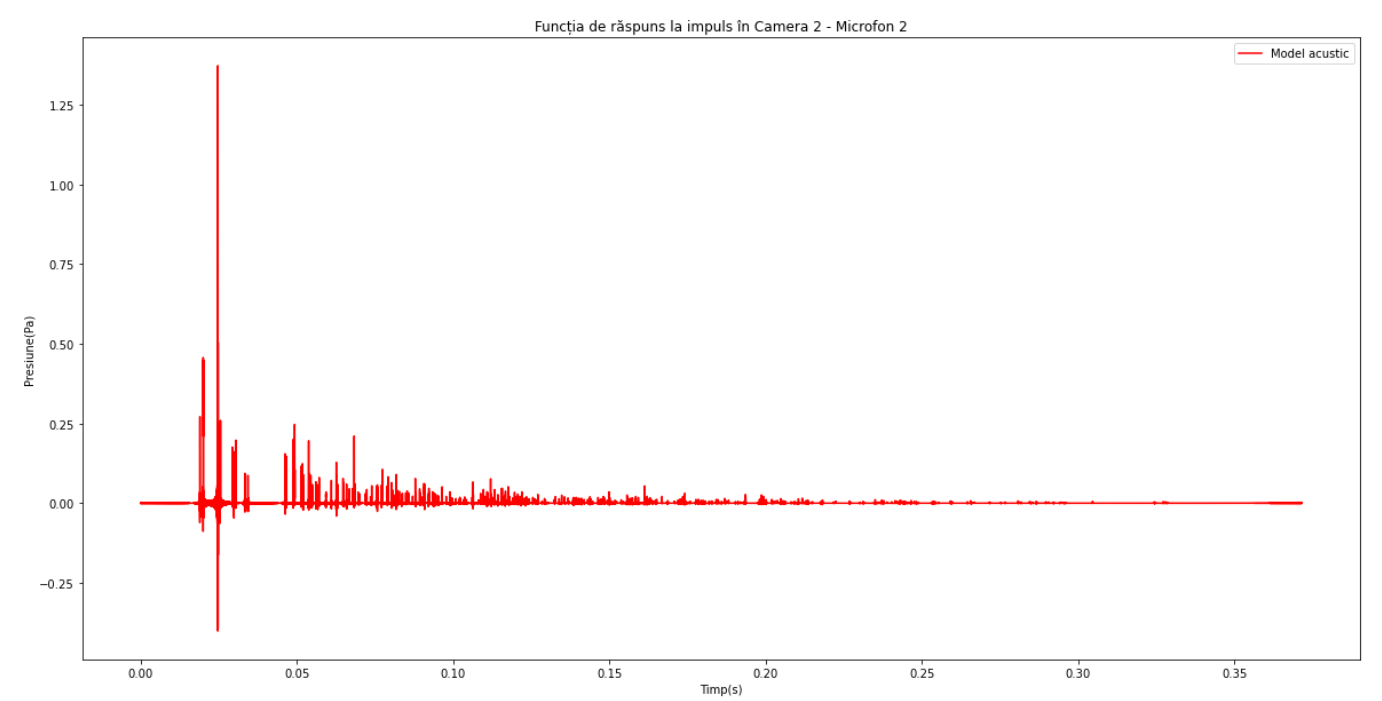
\includegraphics[width=1\linewidth]{imagini/ir.png}
		\caption{Funcția de rășpuns la impuls pe $M2$ în Camera 2}
		\label{ir}
	\end{figure}
	
	Pentru a putea analiza care este diferența de timp cu care ajunge semnalul pe microfoane am realizat un experiement care presupune desenarea tuturor punctelor obținute după pasul de convoluție. În Figura \ref{Fig25} putem observa semnalele rezultate pe toate microfoanele din Camera 2, unde semnalul ajunge cel mai repede pe microfonul 1, fiind la o distanță de 2.56m de sursă, apoi la o distanță foarte mică de timp pe microfonul 0, aflat la 3.07m de sursă, iar în cele din urmă ajunge pe microfonul 2, care este plasat la o distanță de 13.19m de sursă. Concluzionând, cu cât microfonul se află mai departe de sursa audio, cu atât razele vor parcurge un drum mai lung în încăpere și sunetul va ajunge mai târziu pe microfon.
		
	\begin{figure}[!htb]
		\centering
		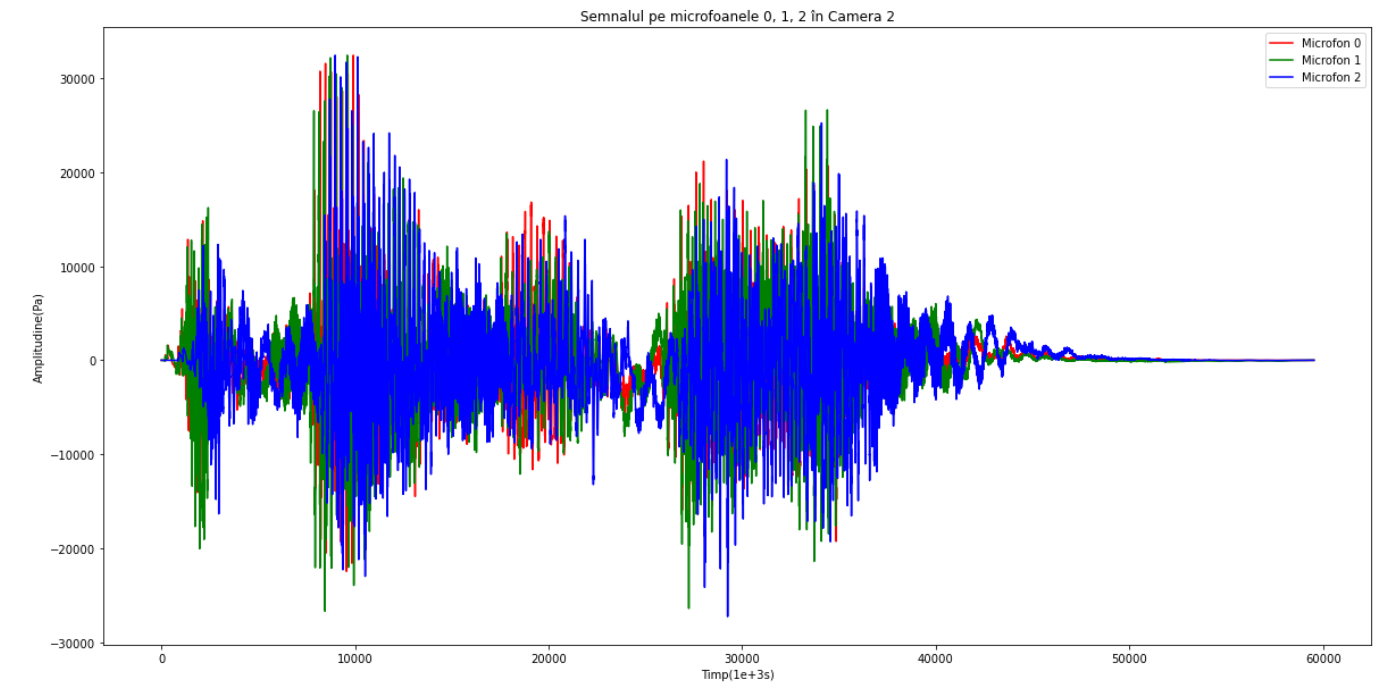
\includegraphics[width=1\linewidth]{imagini/sound.png}
		\caption{Semnalele rezultate pe microfoanele $M0, M1, M2$ în Camera 2}
		\label{Fig25}
	\end{figure}
		
	În contextul unei aplicații în care sunt implicate foarte multe calcule o etapă foarte importantă a acesteia o reprezintă testarea. Acest lucru a fost realizat utilizând Unity Test Runner care folosește o integrare Unity a bibliotecii NUnit, bibliotecă open-source de testare a unităților pentru platforma .Net. Un unit test testează o singură unitate de cod. Acesta trebuie proiectat astfel încât să valideze un fragment mic, logic și să ateste că acea bucată de cod va funcționa exact așa cum ne așteptăm în orice moment.
	
	\begin{figure}[!htb]
		\centering
		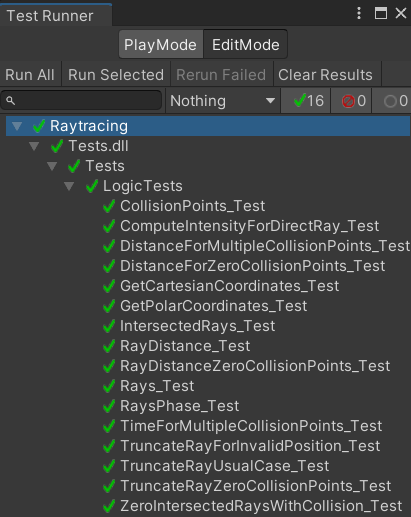
\includegraphics[width=6cm]{imagini/teste1.png}
		\caption{Unit testele aplicației}
		\label{teste}
	\end{figure}
	
	Ca să ne putem asigura de corectitudinea calculelor realizate în cadrul modelului acustic au fost realizate o serie de unit teste menite să verifice anumite situații generale și particulare precum: validarea formulei de calcul a lungimii unei raze, calculul timpilor, ce se întâmpla atunci când avem 0 puncte de coliziune pentru o rază, corectitudinea formulei de calcul a intensității, validarea transformărilor din coordonate polare în carteziene, dar și invers, selecția razelor, intersecția razelor, etc. Toate aceste teste pot fi vizualizate în Figura \ref{teste}.
	
	Rezultatele din aceste camere sunt impresionante, deoarece chiar și pentru camera mică putem face diferența între sunetul de pe primul microfon și cel de pe al doilea microfon. Mai mult, sunetul obținut folosind modelul realizat de noi pentru al treilea microfon este foarte diferit de celelalte microfoane din cameră, ajungând cu un decalaj de timp semnificativ.


\section{Validarea modelului acustic folosind Simcenter 3D}

	Atunci când vorbim despre o aplicație ce propune crearea unui model acustic pentru simularea sunetului în încăperi este foarte important să ne ridicăm problema validării acestuia folosind de exemplu un software similar existent pe piață. În cadrul acestui studiu pentru a fi verificată corectitudinea și validitatea acestui soft am realizat o serie de unit teste ce au fost prezentate în capitolul anterior și, mai mult de atât, am realizat o serie de comparații cu software-ul Simcenter 3D.
	
	Simcenter 3D este o platformă de simulare complet integrată pentru modelarea, simularea și analizarea produselor și sistemelor complexe de inginerie. Platforma include soluții puternice de simulare pentru mai multe discipline, inclusiv analize structurale, acustice, de flux, termice, de mișcare și compoziție, precum și optimizare și simulare multifizică. Software-ul își propune să permită simulărilor să joace un rol timpuriu în procesul de proiectare, ducând la creșterea calității, eficienței și inovației.
	
	Simcenter 3D Acoustics Modeling include toate funcționalitățile necesare pentru a crea, în mod eficient, o geometrie de domeniu fluid prin înfășurarea unei suprafețe cu un mesh structural și/sau un model complet de asamblare CAD.
	
	În cazul simulării acustice Simcenter oferă o bibliotecă extinsă de modele precise pentru estimarea surselor de zgomot aeroacustice, inclusiv modele de stare staționară, modele directe, modele de propagare și rezolvarea ecuațiilor de perturbare acustică. Zgomotul aeroacustic indus de flux este o componentă semnificativă a semnăturii acustice a unui vehicul sau a altor produse. Prezicerea și înțelegerea mecanismelor de generare a zgomotului, localizarea surselor de sunet, identificarea căilor de transmisie și prezicerea răspunsului acustic al sistemului este cheia unui bun design acustic.
	
	Frecvențele care trebuie calculate folosind Simcenter 3D pot fi controlate în totalitate de către utilizator. Acestea pot fi definite manual sau preluate automat din vibrațiile structurale. Într-o interfață grafică de utilizator flexibilă (GUI), utilizatorul poate controla și calcula cantități acustice. Acesta poate analiza rezultatele pentru grupuri de elemente sau microfoane individuale.
	
	Modelul de simulare este verificat automat înainte de exportul în
	solver. Se verifică consistența mesh-ului, materialului și proprietăților. Feedback-ul utilizatorului este furnizat pentru a evita erorile înainte de rezolvare.
	
	Pe lângă funcționalitățile standard de postprocesare pentru vizualizarea
	cantităților acustice precum presiunea, intensitatea și viteza, scenarii specifice pot fi create pentru a filtra și afișa în mod eficient rezultatele funcțiilor legate de microfoane.
	
	Ca să putem realiza o serie de comparații am folosit ambele software-uri și am construit aceeași cameră, poziționând identic sursa audio și microfoanele. Ambele modele acustice au folosit aceeași configurație pentru datele de intrare și au fost urmărite cu mare atenție datele de ieșire. Versiunea de Simcenter ce a fost utilizată pentru această validare a fost Simcenter 3D 2021.1. 
	
	Pentru validarea modelului acustic am creat o cameră rectangulară, folosind ambele soft-uri, cu dimensiunile: 30m lățime, 30m lungime și 15m înălțime, unde am plasat sursa $S$ la poziția $S(0, 2.5,0)$, iar microfoanele au fost așezate astfel: 
	
	\begin{itemize}
		\utb $M0(2, 1.6, 1.7)$, fiind la distanța de 3.07m de sursă
		
		\utb $M1(-1.5, 1.2, 1.7)$, fiind la distanța de 2.56m de sursă
		
		\utb $M2(1, 2, 13)$, fiind la distanța de 13.19m de sursă
	\end{itemize}
	
	În Figura \ref{asemanatoare} putem observa că cele două camere sunt similare, folosesc același sistem de coordonate, sursa și microfoanele sunt poziționate identic.
		
	\begin{figure}[!htb]%
		\begin{subfigure}[b]{.48\textwidth}
			\centering
			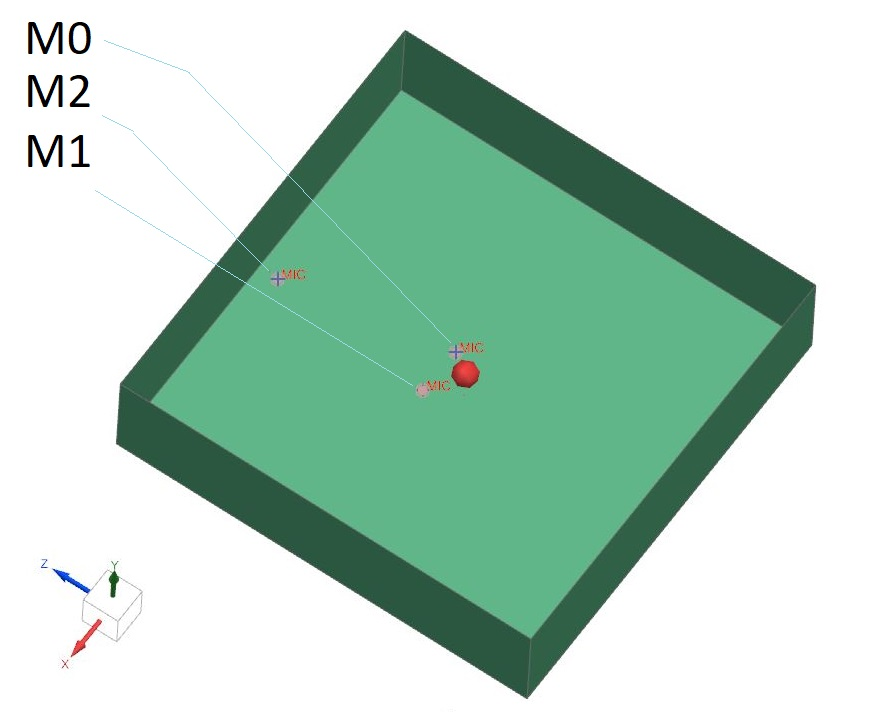
\includegraphics[width=1\linewidth]{imagini/room_view.jpg} 
			%\label{fig:sub-fig}
		\end{subfigure}
		\hfill
		\begin{subfigure}[b]{.48\textwidth}
			\centering
			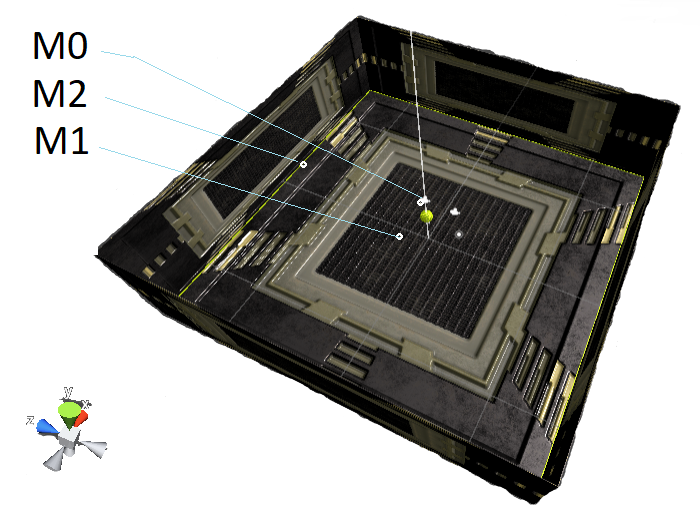
\includegraphics[width=1\linewidth]{imagini/room.png}
			%\label{fig:sub-second}
		\end{subfigure}
		
		\caption{Camerele realizate folosind ambele software-uri}
		\label{asemanatoare}	
	\end{figure}

	
	Vom considera pentru ambele situații c\u{a} densitatea aerului, $\rho_{aer}$, are valoarea $1.2041\dfrac{kg}{m^3}$, iar viteza sunetului prin aer, $c_{aer}$, este $343.21\dfrac{m}{s}$, pentru o temperatur\u{a} constant\u{a} de $20^{\circ}C$.

	Ambele software-uri permit crearea celor două încăperi, crearea unei surse audio și a unor microfoane statice, setarea numărului maxim de reflexii, setarea lungimii maxime a unei raze, setarea pasului de frecvență, folosirea unei melodii, setarea puterii. Diferența dintre cele două software-uri este că Simcenter nu permite setarea numărului de raze ce va fi distribuit în încăpere. Din acest motiv am încercat să găsim un echivalent pentru numărul de raze ce trebuie trasate în încăpere folosind modelul acustic propus de această lucrare. Configurația folosită va fi:
	
	\begin{itemize}
		\utb 1 000 000 de raze distribuite uniform în cazul modelului acustic propus de această lucrare
		
		\utb maxim 10 reflexii pentru o rază
		
		\utb 200m distanța maximă pe care o rază o poate parcurge
		
		\utb 8192Hz numărul de pași de frecvență
	\end{itemize}	

	Configurația folosită pentru camera realizată folosind software-ul Simcenter 3D poate fi viuzalizată cu ajutorul Figurii \ref{config}. Pentru acest software au fost setate dimensiunile potrivite pentru încăpere, numărul maxim de reflexii, distanța maximă, dar și sistemul de coordonate. Putem observa că Simcenter permite utilizarea unor opțiuni mai complexe decât software-ul propus de aplicația descrisă în această lucrare, câteva dintre aceste elemente fiind: opțiunea de a permite difracții 2D și 3D, shimbarea sistemului de coordonate, punerea în evidență a rezultatelor sub mai multe forme, dar și altele.
	
	\begin{figure}[!htb]%
		\begin{subfigure}[b]{.6\textwidth}
			\centering
			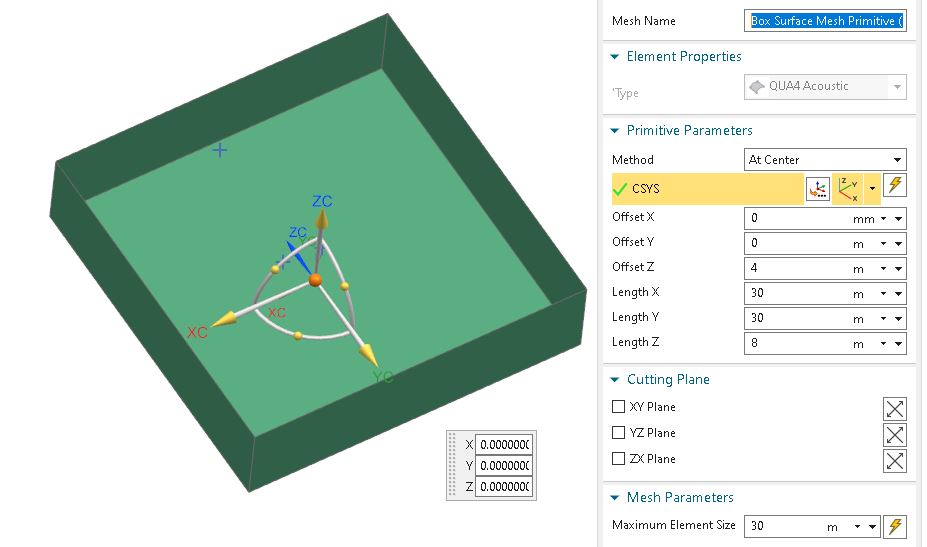
\includegraphics[width=1\linewidth]{imagini/room_primitive.jpg} 
			%\label{fig:sub-fig}
		\end{subfigure}
		\hfill
		\begin{subfigure}[b]{.3\textwidth}
			\centering
			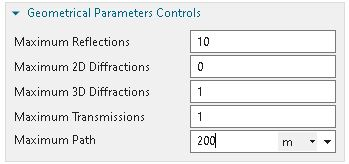
\includegraphics[width=1\linewidth]{imagini/solver_params.jpg}
			%\label{fig:sub-second}
		\end{subfigure}
		
		\caption{Configurația folosită pentru software-ul Simcenter 3D}
		\label{config}	
	\end{figure}
	
	Numărul de raze obținut de modelul vizat de această lucrare pe microfonul $M2$ este 1143, iar numărul de raze care ajunge pe microfonul $M2$ folosind Simcenter este 1400. Conform acestor configurații putem observa similaritatea rezultatelor obținute folosind ambele software-uri urmărind Figura \ref{Fig29}, Figura \ref{Fig26} și Figura \ref{Fig27}.
	
	\begin{figure}[!htb]
		\centering
		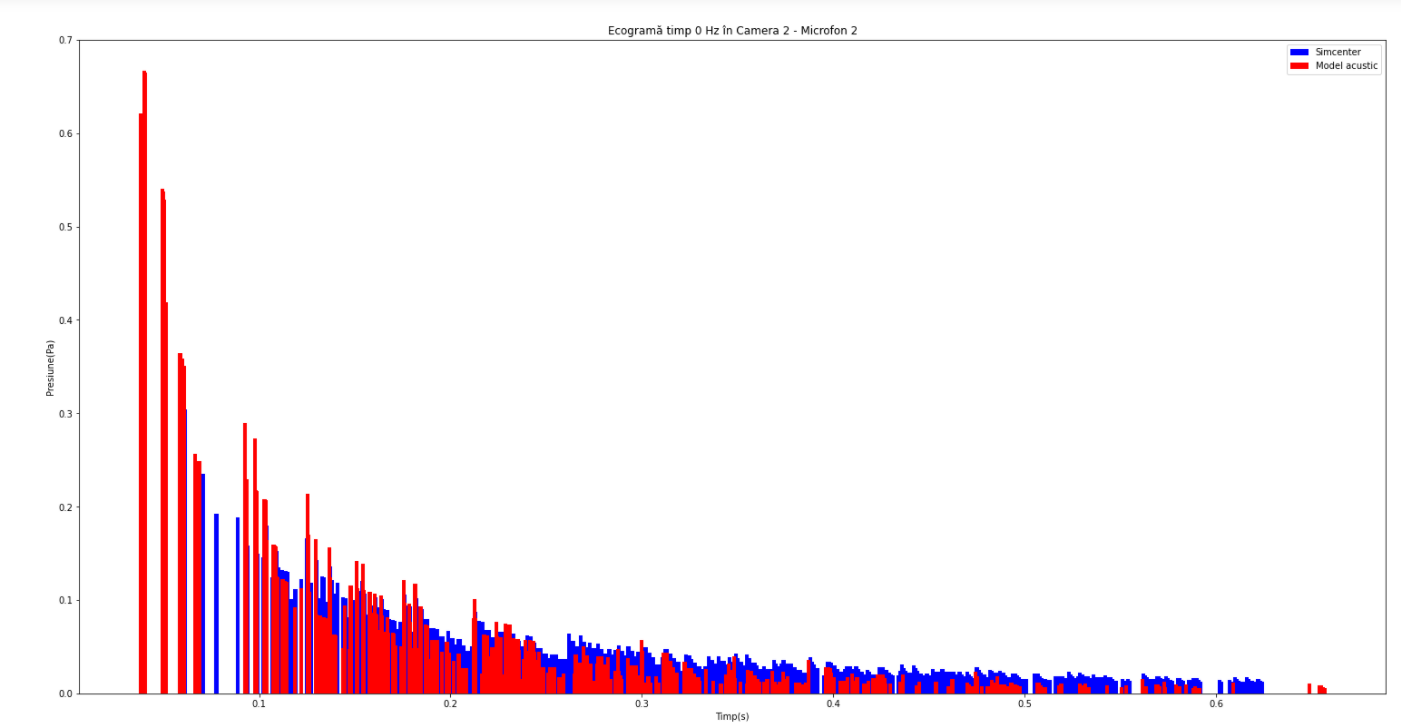
\includegraphics[width=1\linewidth]{imagini/eco_3.png}
		\caption{Ecogramă timp pe microfonul $M2$}
		\label{Fig29}
	\end{figure}

	În cazul ecogramei de timp prezentate în Figura \ref{Fig29}, diferențele de rezultate se explică prin faptul că în Simcenter 3D se folosește un model adaptiv de Ray Tracing care este mai precis. Totuși, pe ecograma se poate observa că nivelul de presiune de la primul impact este același, iar pentru restul impacturilor nivelul este asemănător (diferențele provin din numărul diferit de raze și din traiectoriile diferite). Statistic, pentru un număr suficient de mare de raze din punct de vedere acustic diferențele ar trebui să fie neglijabile.
	
	\begin{figure}[!htb]
		\centering
		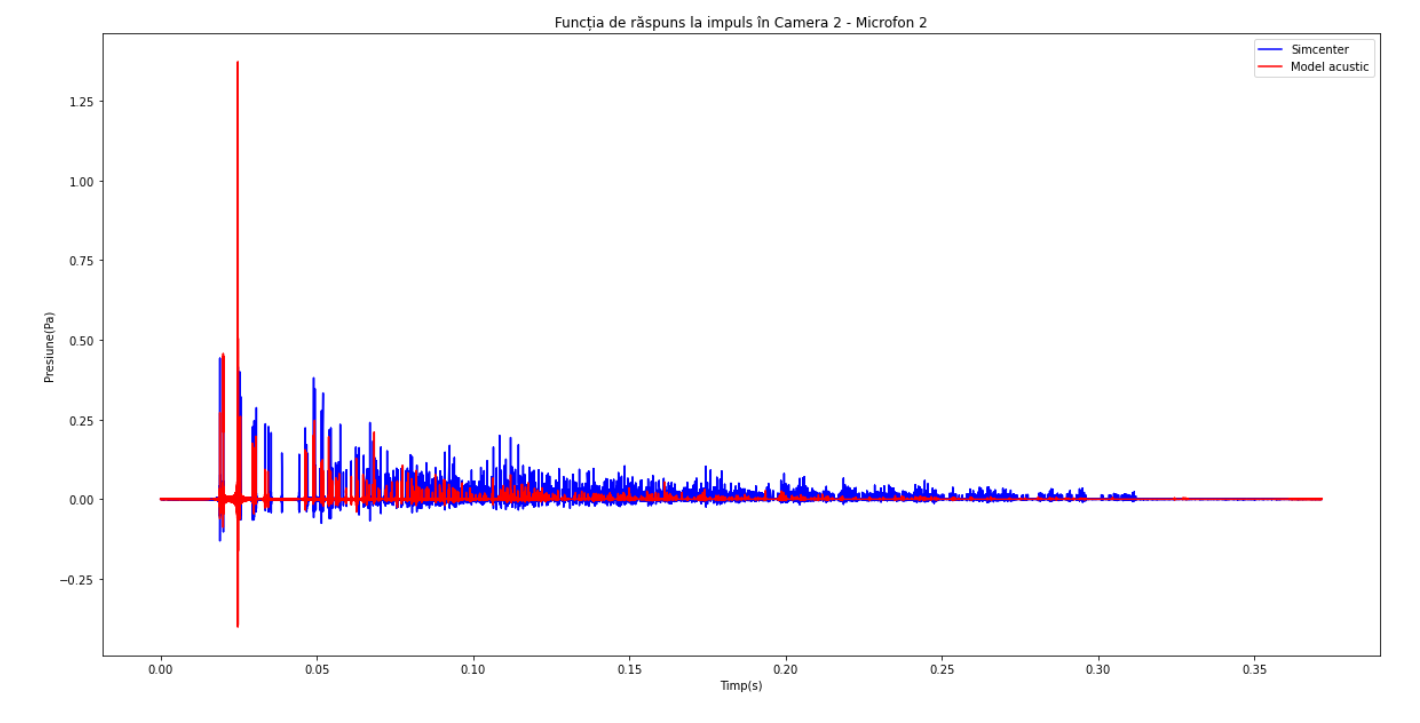
\includegraphics[width=1\linewidth]{imagini/ir_3.png}
		\caption{Funcția de răspuns la impuls pe $M2$}
		\label{Fig26}
	\end{figure}

	Graficul de răspuns la impuls arată amplitudinea undei sonore în timp. Datele utilizate pentru a desena acest grafic sunt produse de un microfon, care probează amplitudinea sunetului la intervale de timp uniform distanțate.

	Precum putem observa în Figura \ref{Fig26}, cele două funcții de răspuns la impuls au valori similare, cu excepția valorii de vârf. Această valoare de vârf diferită este explicată prin faptul că în cazul modelului acustic propus de acest studiu avem 3 raze ce au dimensiuni și căi similare, creând astfel 3 unde care sunt în fază și care își însumează astfel valorile obținând valoarea de vârf din grafic.
	
	Figura \ref{Fig27} prezintă graficul de Frecvență-Magnitudine și graficul Frecvență-Fază cu ajutorul cărora putem reconstrui sunetul audio. Cu ajutorul primul grafic putem să ne dăm seama care este magnitudinea în funcție de frecvență, iar cu ajutorul celui de-al doilea grafic calculăm cât de defazată este o undă sonoră de-a lungul tuturor frecvențelor.
	
	\begin{figure}[!htb]%
		\begin{subfigure}[b]{1\textwidth}
			\centering
			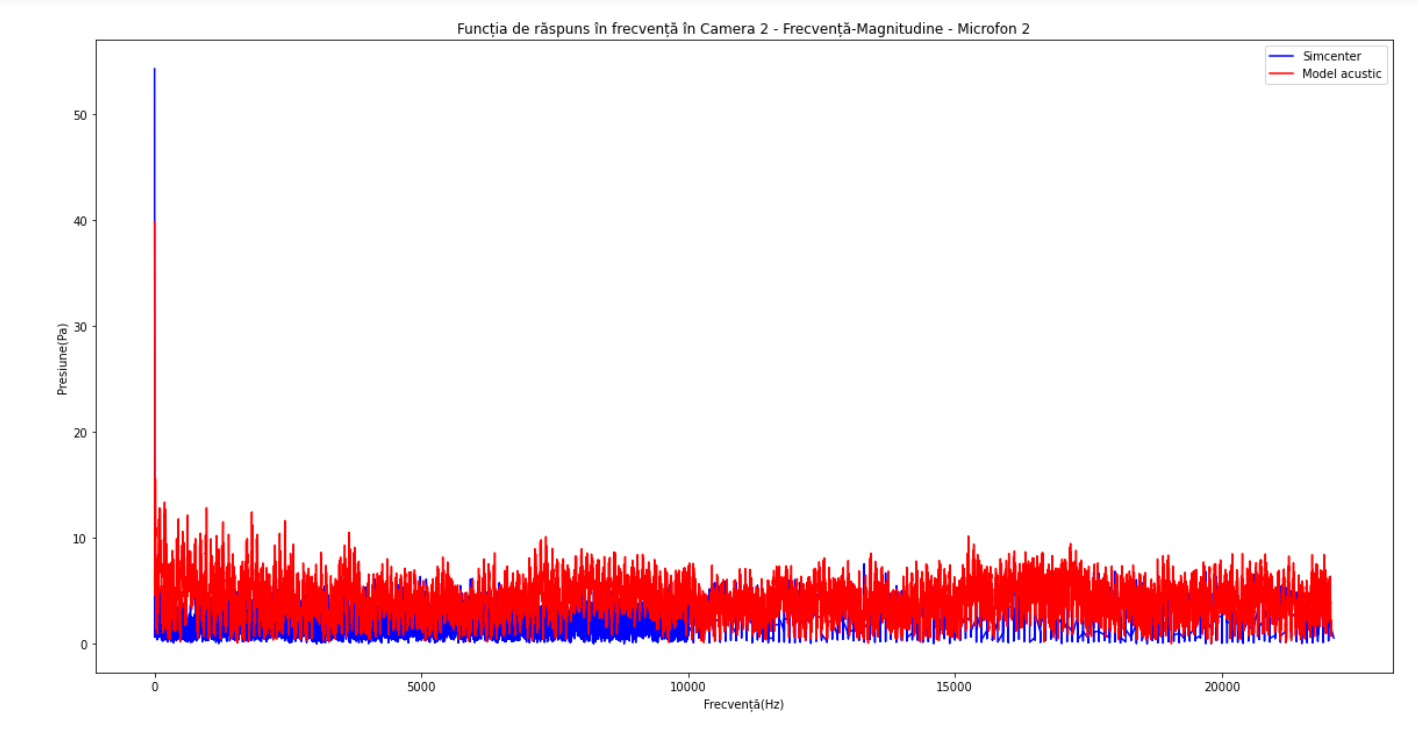
\includegraphics[width=1\linewidth]{imagini/fr_faza_2.png} 
			\caption{Grafic Frecvență-Magnitudine pentru $M2$}
			%\label{fig:sub-fig}
		\end{subfigure}
		\vfill
		\begin{subfigure}[b]{1\textwidth}
			\centering
			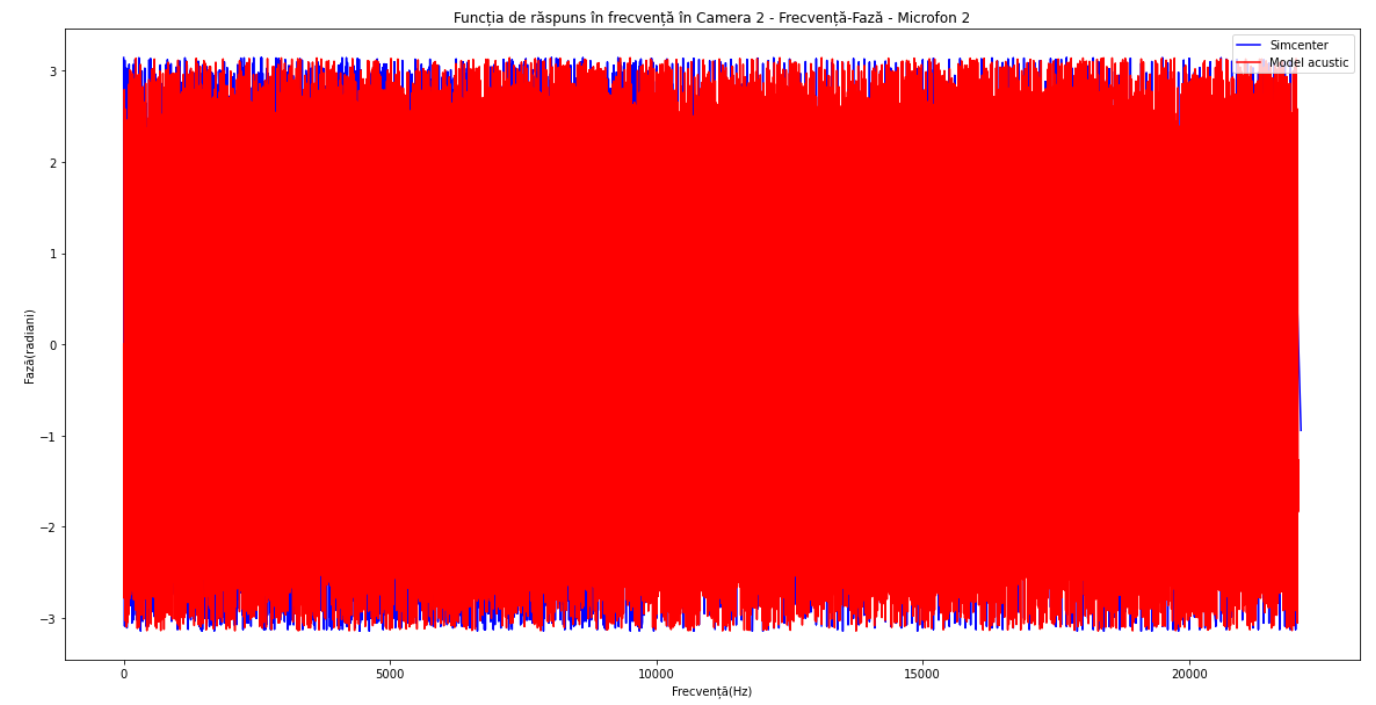
\includegraphics[width=1\linewidth]{imagini/fr_mag_2.png}
			\caption{Grafic Frecvență-Fază pentru $M2$}
			%\label{fig:sub-second}
		\end{subfigure}
		
		\caption{Rezultat Magnitudine-Fază-Frecvență pe $M2$}
		\label{Fig27}	
	\end{figure}

	Considerând toate aceste rezultate prezentate anterior putem să concluzionăm că modelul acustic propus de această lucrare este unul valid, datorită faptului că a trecut cu succes peste toate comparațiile realizate folosind Simcenter 3D. 



	\chapter{Concluzii}
		\section{Concluzii generale}	
	
	Acest studiu propune un model acustic care vine în sprijinul inginerilor acustici pentru a-i ajuta să poziționeze sursele audio și microfoanele atunci când creează încăperi precum hale, amfiteatre, aeroporturi în parametrii acustici normali. 
	
	Modelul acustic propus de noi este unul eficient, care poate fi adaptat și utilizat în contextul oricărui spațiu interior pentru a ajuta la construirea unei camere cu parametrii optimi pentru a crea confortul de care oamenii au nevoie.
	
	Această lucrare necesită ca etapele să fie efectuate secvențial, deoarece ieșirea unui pas este intrarea pasului următor. Calculul geometric este deosebit de important deoarece dictează adesea eficiența algoritmului. Conform complexităților de timp prezentate anterior, putem observa că calculul geometric și calculul fizic au complexitate de timp liniară, iar post-procesarea datelor se realizează în $n\log_2 n$ operații.
	
	Modelul acustic este unul standalone, deci permite decuplarea sa de interfața realizată cu ajutorul platformei Unity și folosirea acestuia în funcție de dorințele și nevoile utilizatorului. Interfața aplicației permite vizualizarea tuturor razelor de pe microfoane, dar și vizualizarea unei singure raze.
	
	În cadrul aplicației au fost realizate teste pentru a verifica corectitudinea calculelor și anumite situații particulare folosind unit teste și, mai mult de atât, a fost și validată folosind Simcenter 3D, o platformă de simulare complet integrată pentru modelarea, simularea și analizarea produselor și sistemelor complexe de inginerie.
	
	Un aspect foarte important este faptul că acest model acustic consideră absorbția sunetului ținând cont de suprafețele pe care le întâlnește o rază pe traiectul ei, fapt care aduce soluția propusă mai aproape de realitate.
	
	Aplicația realizată nu se limitează doar la prezent, ci este o aplicație pentru care se pot face multiple îmbunătățiri prin realizarea unei simulări binaurale sau adăugarea fenomenului de difracție, dar și altele, fiind astfel orientată spre viitor oferind posibilitatea de dezvoltare continuă.
	
	
\section{Concluzii personale}
	
	Mi-am dorit ca prin această lucrare să modelez o soluție pentru o problemă inspirată din realitate, care să fie de actualitate și să necesite un proces de învățare și dezvoltare continuu. Am reușit să dobândesc noțiuni din domeniul ingineriei acustice pornind de la ce este sunetul până la a înțelege cum se propagă sunetul în lumea reală și ce fenomene produce acesta, pentru a putea modela aceste comportamente fizice în contextul aplicației mele.
	
	A fost cu adevărat o lucrare provocatoare care m-a determinat să învăț atât noțiuni teoretice, cât și cum se folosește platforma Unity și cum pot integra alte biblioteci într-o aplicație Unity, să ies din sfera mea de confort și să dezvolt lucruri cu adevărat impresionante din punct de vedere programatic și ingineresc.
	
	Evident, au existat momente în care am întâmpinat greutăți în dezvoltarea acesteia, printre aceste momente se numără: pasul în care am trecut de la realizarea calculelor în domeniul timpului la realizarea calculelor în domeniul frecvențelor și calculul intensităților. Poate cel mai dificil pas a fost realizarea GUI-ului, pentru că nu cunoșteam platforma Unity suficient de bine pentru a ști cum se realizează meniurile și a fost nevoie de mult timp pentru a învăța cum pot face acest lucru astfel încât acesta să fie redimensionabil.
	
	Este o aplicație pe care îmi doresc să o dezvolt și în continuare pentru că aceasta este situată într-un domeniu care permite acest lucru prin adăugarea unor elemente precum difracția, simularea binaurală și chiar îmbunătățirea acesteia din punct de vedere al timpului de execuție prin schimbarea modului de calcul geometric sau mutarea calcului pe GPU. Toate aceste elemente aducând modelul acustic mai aproape de realitate.
	
\section{Dezvolt\u{a}ri ulterioare}

	Ca orice model acustic, acesta poate include îmbunătățiri precum abordarea altor tehnici de calcul geometric. O posibilă soluție ar putea fi începerea trasării razelor pornind de la microfoane la sursa audio. O altă soluție ar putea fi păstrarea distribuției razelor cu modificarea că atunci când o rază întâlnește o suprafață se sparge în mai multe raze. Mai mult decât îmbunătățirea modului de simulare a geometriei camerei, se poate realiza o  îmbunătățire generală din punct de vedere al timpului computațional al aplicației, astfel încât toate calculele ar putea fi mutate pe GPU.
	
	Pentru a îmbunătății aplicația se poate considera introducerea fenomenului de difracție în aplicație, care reprezint\u{a} schimbarea local\u{a} \^{i}n direc\c{t}ia propag\u{a}rii undelor sonore trec\^{a}nd de marginea unui obstacol.
	
	Se poate lua în considerare și simularea binaurală care reprezint\u{a} o metod\u{a} de a realiza semnale binaurale la ambele urechi ale receptorului \^{i}n spa\c{t}ii inexistente prin intermediul unui model. Pentru fiecare microfon se vor considera două puncte în locul unuia ca și cum ar fi urechile omului.
	
	O altă abordare posibilă ar fi să ținem cont si de absorbția aerului, nu doar de absorbția suprafețelor din încăperi, fapt care ar putea îmbunătății rezultatele pentru încăperile de dimensiuni mari sau atunci când vorbim despre frecvențe înalte. 
	
	\begin{thebibliography}{99.}%

\bibitem{elorza} David Oliva Elorza, \textit{Room acoustics modeling using the raytracing method: implementation and evaluation}, Licentiate Thesis, University of Turku, 2005

\bibitem{fft} Steve Haynal, Heidi Haynal, \textit{Generating and Searching Families of FFT Algorithms}, Journal on Satisfiability, Boolean Modeling and Computation 7, 2011

\bibitem{jeong} Jeong Cheol-Ho, Ih Jeong-Guon, Rindel Jens Holger, \textit{Consideration of Wall Reflection and Diffraction in the Room Acoustic Prediction Using the Phased Beam Tracing Method}, 9th Western Pacific Acoustics Conference, Seoul, Korea, 2007

\bibitem{soundPress} Alexander Sengpiel, \textit{Conversion: Sound pressure to Sound intensity and vice versa}, Tutorium, Berlin, 2013

\bibitem{helmoltz} Jonathan Andrew Hargreaves, Yiu Wai Lam, \textit{An Energy Interpretation of the Kirchhoff-Helmholtz Boundary Integral Equation and its Application to Sound Field Synthesis}, Acta Acustica united with Acustica, 2014

\bibitem{unity} Axon Samuel, \textit{Unity at 10: For better- or worse- game development has never been easier}, Ars Technica, 2016

\bibitem{chris} Christoffer A. Weitze, Clau Lynge Christensen, Jens Holger Rindel, Anders Christian Gade, \textit{Computer Simulation of the Acoustics of Mosques and Byzantine Churches}, 17th ICA, Rome, Italy (2001)

\bibitem{kirchoff} Jonathan Andrew Hargreaves, Yiu Wai Lam, \textit{An Energy Interpretation of the Kirchhoff-Helmholtz Boundary Integral Equation and its Application to Sound Field Synthesis}, Acta Acustica united with Acustica (2014)

\bibitem{limbaj} Lucian M. Sasu, \textit{Medii vizuale de programare}, 2020

\bibitem{temperaturaTabel} Effect of temperature on properties of air, 24 noiembrie 2020

https://en.wikipedia.org/wiki/Speed\_of\_sound

\bibitem{snell} Legea lui Snell- Snell's law, 8 decembrie 2020

https://ro.qaz.wiki/wiki/Snell\%27s\_Law

\bibitem{fibo} How to evenly distribute points on a sphere more effectively than the canonical Fibonacci Lattice, 14 decembrie 2020

http://extremelearning.com.au/how-to-evenly-distribute-points-on-a-sphere-more-effectively-than-the-canonical-fibonacci-lattice/

\bibitem{raycast} Physics.Raycast din Unity, 15 decembrie 2020

https://docs.unity3d.com/ScriptReference/Physics.Raycast.html 

\bibitem{intersectie} Intersec\c{t}ia unei sfere cu o linie, 22 decembrie 2020

http://www.ambrsoft.com/TrigoCalc/Sphere/SpherLineIntersection\_.html

\bibitem{square} Legea Pătratului Invers, 25 decembrie 2020,

https://ro.xcv.wiki/wiki/Inverse-square\_law

\bibitem{python} Biblioteca matplotlib, 20 ianuarie 2021

https://pypi.org/project/matplotlib/

\bibitem{nwaves} Biblioteca NWaves, 3 decembrie 2020

https://github.com/gkngkc/UnityStandaloneFileBrowser

\bibitem{standalone} Biblioteca StandaloneFileBrowser, 10 decembrie 2020

https://github.com/gkngkc/UnityStandaloneFileBrowser

\bibitem{xcharts} Biblioteca XCharts, 15 decembrie 2020

https://github.com/monitor1394/unity-ugui-XCharts/blob/master/Assets/XCharts/ README.md

\bibitem{istorie} O scurtă istorie a acusticii, 20 august 2020

https://www.britannica.com/science/acoustics

\bibitem{triton} Proiectul Triton realizat de Microsoft, 20 iulie 202

https://www.microsoft.com/en-us/research/project/project-triton/

\bibitem{simcenter} Simcenter 3D, 2 ianuarie 2021

https://www.plm.automation.siemens.com/global/en/products/simcenter/


\bibitem{conf} A 14-a conferință internațională despre știința cunoașterii, inginerie și management (KSEM 2021), 8 iunie 2021

http://www.cloud-conf.net/ksem21/index.html

\end{thebibliography}

	
	\newpage
	
\end{document}